\chapter{What Drives State-Sponsored Violence?: Evidence from Extreme Bounds Analysis and Ensemble Learning Models}
\label{chap:killings}

\section{Introduction}
\label{sec:intro4}

Since the end of World War II, mass killings, genocides, and politicides have claimed over 34.5 million lives \citep{marshall2017pitf}.\footnote{Genocide and politicide are the attempted intentional destruction of communal or political groups, respectively \citep[see][]{harff1988toward}. Mass killing includes these atrocities, as well as attacks against civilians that result in at least 1,000 deaths but are not intended to destroy a particular group \citep[see][]{ulfelder2008assessing}. While some conflate the logic of these types of atrocities \citep[e.g.,][]{rummel1995democracy, valentino2004draining}, others claim genocide and politicide follow a different logic from other forms of government violence \citep{kalyvas2006logic,stanton2015regulating}. For discussion on these important differences in conceptualisation see \citet[]{straus2007second} and \citet{finkel2012macro}.} The international community has responded with an effort to prevent further state-sponsored mass murder by strengthening laws against war crimes, genocide, and crimes against humanity. Furthermore, the United Nations established a Special Adviser on the Prevention of Genocide and recognised its members' responsibility to protect civilian populations within and outside their own borders. Yet, such atrocities still occur. Recently, President al-Assad of Syria has massacred tens of thousands of civilians during the Syrian Civil War \citep{goldman2017nyt}. Similarly, South Sudan's President Kiir is actively starving and killing civilians from dissident and rival tribes \citep{nichols2017reuters}. While there is some evidence that such atrocities may be declining since the Cold War \citep{valentino2014we}, the international community has been far from successful in realising slogans like ``Never Again'' and ``Not on My Watch'' \citep{cheadle2007not}.
	
Ultimately, effective prevention requires us to understand why these atrocities occur. In this vein, the academic community has laboured tremendously to establish empirically-based theories as to why governments engage in brutality against their civilian populations. Indeed, since 1995, there have been over 45 quantitative political science articles focused on explaining government-sponsored killing of civilians. Overall, the mass violence literature agrees that government atrocity follows an opportunity logic: as threat increases, so does the likelihood of atrocity, if the costs to such violence are not prohibitive. However, there is little consensus on what factors influence the level of threat or costs a regime faces. Part of the reason for this uncertainty is that scholars use very different model specifications when testing their arguments, thus small changes in model parameters could influence the robustness of empirical results and the inferences I draw from these findings.
	
To overcome these limitations and provide a better understanding of government atrocity, I employ extreme bounds analysis and random forests to identify the most robust determinants of state-sponsored atrocities. My approach is similar to Hegre and Sambanis' (\citeyear{hegre2006sensitivity}) seminal analysis on the causes of civil war onset, but like \citet{bell2015examining}, \citet{hill2014empirical} and \citet{jones2018there}, I provide additional tests to verify whether complex interactions and nonlinearities are driving the statistical results. More broadly, my goals are: 1) to examine whether the current quantitative scholarship is able to identify robust explanators of mass atrocities; 2) to evaluate how those variables compare to each other in explaining power. 

While recent studies of mass killings have progressively adopted stronger identification strategies, the majority of the literature consists of cross-country regressions. While the importance of micro-level causal designs have been largely discussed \citep[e.g.][]{angrist2008mostly,imbens2015causal}, large-$n$ analyses also have strong benefits that are often overlooked. For instance, quantitative studies allow scholars to assess the external validity of specific explanatory mechanisms. Additionally, these studies provide a safeguard against the perils of selecting on the dependent variable, a bias that can severely distort regression results \citep{bell2015examining,king1994designing}. Cross-national comparisons also show how structural factors condition immediate causes of mass violence. Atrocities are multicausal phenomena, and large-$n$ studies can point to interactions that scholars would otherwise miss. In this specific study, there is the additional advantage of running all the models with the same dependent variable, what constitutes an effective method of replication of the original findings.

In conducting this analysis, I address three debates in the mass violence literature:
	
\begin{enumerate}
 \item Why do some governments engage in mass killings, genocides, or politicides? This is the primary question asked by activists, policymakers, and scholars in this field of research. 
 \item Does the logic underpinning government decision-making follow different patterns during peacetime and wartime? Recent research suggests that government atrocity occurs predominantly during periods of civil unrest \citep{harff2003no} which has led some scholars to restrict their analyses to only periods of civil war \citep[e.g.,][]{colaresi2008kill, valentino2004draining} or concentrate on predicting both the onset of civil war and atrocity \citep{goldsmith2013forecasting}. Yet, others estimate models of all country-years \citep[e.g.,][]{krain1997state, montalvo2008discrete}, raising questions of how well these studies speak to each other.
 \item Is there a difference in logic between those atrocities labelled as genocide or politicide, compared to other mass killings? While the Political Instability Task Force \citep{marshall2017pitf} provides the most widely used data on government atrocity, others provide data with much more lenient inclusion criteria \citep[e.g.,][]{stanton2015regulating, ulfelder2012forecasting}. These differences in definition of atrocity have led to divergent results, raising questions about important determinants of government behaviour \citep[for discussion, see][]{straus2007second, uzonyi2016domestic, wayman2010explaining}.
\end{enumerate}

My analysis tests the sensitivity of 40 variables on a sample of 177 countries from 1945 to 2013. My findings partially confirm previous research -- poor, unstable countries are more likely to witness the regime employ atrocity \citep[e.g.,][]{goldsmith2013forecasting,harff2003no,krain1997state}. However, many of the factors scholars often cite as observable indicators of such instability -- regime transitions, coups d'état, the presence of militias, etc. -- are not good proxies for instability. Thus, policymakers may be looking for the incorrect signs of impending atrocity when seeking to prevent its onset. Furthermore, I find that the conclusions scholars draw regarding the likelihood of government atrocity largely depend on whether they combine peace and war years or just analyse periods of civil wars, as patterns in mass killings differ dramatically across these contexts. Lastly, I find that genocide and politicide follow vastly different patterns of onset than other forms of state-sponsored mass murder. This is further evidence that different logics govern different forms of political violence \citep{stanton2013terrorism}.

Overall, these findings raise concerns about policy options for preventing violence against civilians. If my conclusion is that poor and unstable countries are violent, then preventing atrocity likely requires significant investments of time and resources in state-building, which is often politically and practically infeasible \citep{doyle2006making}.  This analysis contributes significantly to the political violence literature by highlighting the parsimonious nature of the logic behind government atrocity and clearing away much of the empirical clutter surrounding this conclusion. 
	
\section{Empirical Methods}
\label{sec:methods}
	
To conduct my analysis, I began by surveying the quantitative political science literature on the causes of government mass killing since Rummel's (\citeyear{rummel1995democracy}) seminal work on the subject. Counting only published works, I identified 45 articles which employed logit or probit models of mass killing onset in a global sample. I then included all variables that appeared in at least two of these papers in the data set at the country-year unit of analysis for all years from 1945 to 2013. The appendix provides a complete list of the articles I considered and a complete list of the variables I included in my models. Next, I estimated an extreme bounds analysis to determine which variables were the most robust in explaining the onset of government atrocity. Then, I estimated a distributed random forest analysis to see which of the variables best predicted the onset of these atrocities. In this section, I provide more detail on each of these estimation procedures before turning to the results of both analyses in the next section.

\subsection{Extreme Bounds Analysis}
\label{subsec:eba}

The first method I employ to test the robustness of the potential determinants of state-led violence is the extreme bounds analysis (EBA). Researchers have employed EBA to assess the sensitivity of the determinants of civil war \citep{hegre2006sensitivity}, coups d'état \citep{gassebner2016expect}, democratisation \citep{gassebner2013extreme}, economic growth \citep{levine1992sensitivity, sala1997just}, nuclear deterrence \citep{bell2015examining}, and political repression \citep{hafner2005right}. The method is particularly useful when there is no consensus about which covariates belong in the ``true'' regression model \citep[178]{sala1997just} and scholars worry that omitted or unnecessary predictors can bias the model estimates \citep[60]{angrist2008mostly, clarke2005phantom, elwert2014endogenous, spector2011methodological}.

More specifically, the main purpose of EBA is to estimate the distribution of coefficients of each predictor $x$ in an exhaustive combination of regression models with $y$ as a dependent variable. \cite[308]{leamer1985sensitivity} proposed that ``sturdy'' variables are those whose minimum and maximum of their coefficient distribution have the same sign and are situated at a distance from zero. If we are to use the conventional value of $p < 0.05$, the mean of the variable coefficients' distribution should be located at least $1.96$ standard deviations away from zero. 
	
Leamer's criterion is intuitive, but other authors contend it is too strict for most social science applications. \citet{sala1997just} argued that Leamer's EBA would increase the number of false negatives; in other words, it would classify as fragile covariates that are truly associated with the response. In this paper, I use Sala-i-Martin's more flexible version of EBA and consider the whole range of values of $CDF(0)$. I choose to use the whole distribution because the aggregate $CDF(0)$ allows researchers to move away from a binary indicator of robustness and present the estimations with their appropriate degrees of confidence. My focus is the percentage of the variable's cumulative distribution function that is smaller or greater than zero. I do not assume that the CDFs are normally distributed and use Sala-i-Martin's generic model.\footnote{The generic model provides a better fit to the data. Histograms for all coefficients are available in online appendix.} I specify the models as follows:
	
\begin{equation}
\text{\textit{Mass Killing Onset}}_{it} = \beta_{M}M_{it} + \beta_{F}F_{it} + \beta_{Z}Z_{it} + v_{it}
\end{equation}
	
My main dependent variable is \textit{Mass Killing Onset}, which denotes the onset of government-sponsored killings. \citet[2]{ulfelder2008assessing} define a mass killing as ``any event in which the actions of state agents result in the intentional death of at least 1,000 noncombatants from a discrete group in a period of sustained violence''. Respectively, $i$ and $t$ indicate country and year. $M$ is a set of three covariates that are included in every model due to their prominence in the literature \citep{levine1992vale}. In my analysis, $M$ includes the natural logarithm of the GDP per capita to control for income, the Polity IV index to control for level of democracy, and a linear time trend since the last episode of government-led atrocity to account for temporal dependence. $F$ denotes a vector of variables of interest, and $Z$ is a vector of other control variables in addition to those included in $M$. $v$ is the error term. In practice, however, since this research is interested in the effect of all variables in the data set and do not have true control variables, except from $M$, $F$ and $Z$ are interchangeable. I thus only use this notation to help clarify the connection of my analysis to previous conflict scholars who employed similar extreme bounds analysis \citep[e.g.,][]{hegre2006sensitivity,gassebner2016expect}. Following \citet[514]{hegre2006sensitivity}, I lagged the independent variables one year to reduce the risk of endogeneity. 

Although the dependent variable is dichotomous, I use linear probability models in my main analysis. \citet[298]{gassebner2016expect} argue that linear probability models are less prone to convergence problems and their results can be readily interpreted. Since the data are grouped into countries, I also use cluster-robust standard errors.
	 
As a precaution against collinearity, I place a limit on the Variance Inflation Factor (\textit{VIF}) of all regression coefficients. The VIF estimates how much of the variance of each predictor is dependent on the other covariates in a model. A VIF of 1 indicates that the predictor is uncorrelated with the remaining covariates. VIF limits are often arbitrary \citep{bell2015examining,o2007caution}, thus here I use a moderately conservative VIF of 7. As robustness tests, I run the same models without restriction and with different cut-offs.
	
Two variables were omitted from EBA models but included in the machine learning estimations. The first is \textit{democracy}, a dummy variable that indicates whether the country has a Polity IV score equal or higher than 5. The second is \textit{interstate war}, a binary covariate measuring if the country is at war in a given year \citep{sarkees2010resort}. I have decided to omit democracy because of its evident correlation with the Polity measure and interstate war due to its correlation with the dependent variables. EBA models do not converge otherwise.\footnote{This is a typical case of multicollinearity and conceptual overlap. \citet{hlavac2016eba} suggests specifying a set of mutually exclusive variables to avoid the issue. However, as the Polity index is one of the core variables, I decided to drop the binary democracy indicator and use the continuous measure as it provides more details about the effect of political regimes on mass killings. More information available in the appendix.}  Since this problem does not affect machine learning algorithms, the two variables were included in the second set of estimations.
	
Lastly, I depart slightly from Sala-i-Martin's suggested method and do not assign weights to EBA. Although he recommends using goodness-of-fit measures to construct regression weights, I follow \citet{sturm2002robust} and \citet[299]{gassebner2016expect} and use the unweighted version of the CDF instead. Goodness-of-fit indicators are not equivalent to the probability of a given model being true \citep{anscombe1973graphs,king1986not}, and the weights constructed this way are not invariant to transformations in the dependent variable. Moreover, the data set has a number of missing observations, so model comparison measures could be misleading \citep{lall2016multiple}.
	
\subsection{Random Forests}
\label{sub:drf}

I also make use of random forest \citep{breiman2001random} to evaluate whether the empirical results in the mass killings literature are driven by parametric assumptions and model specifications. Random forest is a machine learning algorithm that consists of a combination of individual decision trees. In a classification problem, each decision tree uses a vector of covariates to split the dependent variable into two increasingly homogeneous parts \citep{breiman2001statistical}. However, decision trees are prone to overfitting, i.e., they match the original data set so closely that they tend to perform poorly with new data \citep{dietterich1995comparison,ho1998random}. Random forest, in contrast, avoids this issue by growing a decision tree only to a bootstrap sample of the original data, selecting random features at each split, then aggregating the different trees into a single prediction. If the independent variable is continuous, the algorithm will simply choose the average value of the predictions as the best candidate; if the covariate is discrete, the majority class will be employed. The simple procedure of leaving out some data points and growing separate trees with a random subset of covariates is sufficient to eliminate overfitting \citep[9-10]{jones2015exploratory}.
	
Random forest has many desirable properties, such as ``highly accurate predictions, robustness to noise and outliers, internally unbiased estimate of the generalisation error, efficient computation, and the ability to handle large dimensions and many predictors'' \citep[7]{muchlinski2015comparing}. Thus, random forest allows the researcher to estimate very flexible models with minimal assumptions. Unlike parametric methods such as ordinary least squares or logistic regressions, the analyst does not have to impose any distributional form to the data-generating process. As a result, random forest is able to effectively uncover complex, nonlinear interaction effects in the data without prespecification \citep{jones2015exploratory,jones2018there}. Random forest models complement the extreme bounds analysis in two ways; first, by providing robust additional tests to the parametric estimations, and also by pointing out eventual limitations of the widely-employed modelling techniques in the mass violence literature. 
	
In this paper I use distributed random forest (DRF) to model the data, a slightly modified version of the original random forest algorithm \citep{h2o2017}. The DRF has two additional features that are useful for the purposes of this chapter. Firstly, DRF is optimised for big data, as it grows decision trees on separate cores to speed up computation time. Secondly, in DRF, non-observed cases are not assumed to be missing at random, but rather as values that contain information in themselves. The algorithm assumes that observations are missing for a reason, what is most likely the case with social science data \citep{lall2016multiple}. This is a more conservative approach than assuming that missing cases fit into an underlying parametric distribution.\footnote{For more information about how the distributed random forest algorithm deals with missing observations, please refer to: \href{http://docs.h2o.ai/h2o/latest-stable/h2o-docs/data-science/drf.html}{\texttt{http://docs.h2o.ai/h2o/latest-stable/h2o-docs/data-science/drf.html}} (access: December 2017).}
	
The DRF has a series of hyperparameters that can be tuned to improve its predictive performance. For instance, users can control the number of decision trees in each iteration, how deep trees should grow, and many other options. The interaction between parameters is generally complex and may involve thousands of potential combinations. As an example, a researcher interested in four parameters with 10 values each would have to estimate 10,000 models before deciding which is the most efficient one. Also, machine learning parameters are sensitive to the data at hand, that is, an optimal solution for one problem cannot be readily implemented in another data set \citep{genuer2008random,goldstein2010application,jones2015exploratory}.
	
To address these issues, I perform a grid search to select the most accurate random forest model \citep[123]{cook2017h2o}. I estimate a model for every possible combination of the hyperparameter space to make sure the model results are robust to different specifications. For model selection, I follow the literature on predictive political science and use the area under the ROC curve (AUC) as the model evaluation metric \citep[e.g.,][]{hill2014empirical,ward2010perils,ward2013learning}. Models with higher AUC values are considered more accurate.
	
I add several parameters to the grid search. The first is the number of independent trees to grow in each forest. The starting values are 256, 512, and 1024 trees. The machine learning literature does not provide a heuristic on how large a random forest should be, but \citet[166]{oshiro2012many} affirm that ``from 128 trees there is no more significant difference between the forests using 256, 512, 1024, 2048 and 4096 trees.'' I employ a more conservative approach and start from a higher value that the authors suggest as adding more trees do not reduce prediction accuracy \citep[7]{breiman2001statistical}.
	
The depth of each decision tree also influences the algorithm performance. Deeper trees indicate more complex models, and in general they provide a better fit to the data. Nevertheless, this complexity comes at the risk of overfitting, so deeper trees are not necessarily the most adequate solution for every model \citep[596]{friedman2001greedy,segal2004machine}. In this article, I let the algorithm decide among using 10, 20, or 40 levels for each tree. 
	
I test whether having balanced classes of the dependent variable (mass killing onset) affects the predictive ability of the model. Since the response measure is heavily imbalanced, oversampling the positive responses could potentially improve the results \citep{chawla2004special,del2014use,japkowicz2002class}. 
I also vary how many variables should be considered for each split in the data. The default option is to use $\sqrt{p}$, where $p$ is the number of columns in the data set. As I have 40 covariates of interest, I have selected 5, 6 and 7 variables per split. The DRF uses a majority voting procedure to select which variable is most important. Additionally, the algorithm chooses the percentage of the training set to be modelled by each tree. The default option is 63.2\%, but I include the options of using 50\% and 100\% of the data. Similarly, I give a range of options for choosing how many columns will be included in each tree. The algorithm can randomly choose among 50\%, 90\% or 100\% of the independent variables when estimating a decision tree.

Finally, I use three types of histogram to find optimal split points for each independent variable. Decision trees consider every value of a given independent variable as a potential candidate for a split in the training data. This process is notably time-consuming, and computation time can be significantly reduced at little loss of precision by taking discrete values of the predictor distribution. The DRF algorithm also offers the choice of randomly cycling through all histogram types, including one of the types in each tree estimation. I adopt this ``round robin'' arrangement as it is both computationally efficient and methodologically parsimonious.
	
\section{Results}
\label{sec:results4}

\subsection{Main Model}%
\label{sub:main_model}
	
I endeavour to answer three questions in this analysis: 1) what are the robust predictors of government mass killing, 2) do these predictors differ when considering only cases of civil war, and 3) are genocide and politicide different than other forms of atrocity? Table \ref{tab:eba01} summarises the main EBA results in answering Question 1. The table shows the average coefficient estimate of all regressions for each robust variable along with their mean standard deviations.\footnote{A list of all independent variables and coding rules are available in the appendix.} The table also displays the percentage of regressions that are statistically significant at the 90\% level. $CDF(0)$ represents the cumulative distribution function, which is the area of the distribution that falls above or below zero.\footnote{I show whichever area is the largest. The sign of the average $\beta$ coefficient indicates if most of the cumulative distribution is located above or below zero.} This is my main statistic of interest, and I consider a covariate to be robust if it has a $CDF(0)$ of 0.9 or higher \citep[181]{sala1997just}. Lastly, I report the number of estimated regressions models which included each variable.

\begin{table}[H]
\centering
\begin{tabular}{lrrrrr}
\hline
\textbf{Variable} & \textbf{Avg. $\beta$} & \textbf{Avg. SE} & \textbf{$\%$ Sig.} & \textbf{CDF(0)} & \textbf{Models} \\ \hline
\textit{Base variables} &  &  &  &  &  \\
Log GDP per capita & -0.0091 & 0.0052 & 76.055 & 0.9335 & 226707 \\
 &  &  &  &  &  \\
\textit{Additional variables} &  &  &  &  &  \\
Post-Cold War years & -0.0133 & 0.0085 & 72.845 & 0.9472 & 35614 \\
UCDP civil war onset & 0.0529 & 0.0321 & 52.378 & 0.9441 & 20854 \\
Previous riots & 0.0140 & 0.0100 & 56.242 & 0.9216 & 35614 \\
UCDP ongoing civil war & 0.0172 & 0.0115 & 65.652 & 0.9092 & 20854 \\
Ethnic diversity (ELF) & 0.0184 & 0.0137 & 56.674 & 0.9050 & 35614 \\
Polity IV squared & -0.0002 & 0.0001 & 61.206 & 0.9031 & 35614 \\ \hline
\end{tabular}
\caption{Extreme Bounds Analysis -- Mass Killings (Robust Variables Only)}
\label{tab:eba01}
\end{table}
	
Seven variables pass the EBA criterion and three of them decrease the likelihood of mass killings. First, as widely suggested in the literature, the natural logarithm of GDP per capita is negatively associated with the onset of mass killings \citep[e.g.,][]{besanccon2005relative, easterly2006development,esteban2015strategic}. Second, the post-Cold War years are correlated with lower levels of government violence. Indeed, this finding is in line with several studies that point to a general decline in violence over the last decades, including riots, civil wars, and urban crime \citep{pinker2011better,straus2012wars,valentino2014we}. The third robust variable is the squared term of the Polity IV political regime index. This finding points to a nonlinear relationship between political regime and mass killings, thus providing further evidence that democracy reduces state-sponsored violence \citep{rost2013will,rummel1995democracy} and that regimes that mix democratic with autocratic features have the highest risk of conflict \citep{hegre2001toward,muchlinski2014grievances}.
	
Four variables are robustly and positively associated with Ulfelder and Valentino's (\citeyear{ulfelder2008assessing}) indicator of government-sponsored violence. Onset and continuation of civil wars are correlated with mass killings, but only when I employ the UCDP measures of violent conflict. I find no effect for the variables compiled by the Correlates of War project or \cite{cederman2010ethnic}. Former instances of political turmoil also have a positive coefficient in the models. Moreover, countries with a previous history of riots are more prone to state violence, which suggests that government repression is path dependent \citep[e.g.,][]{gurr2000peoples,harff2003no,krain1997state,nyseth2017re}. The results also show that higher levels of ethnic diversity increase the likelihood of atrocities against civilians. Nevertheless, ethnic diversity does not pass all additional tests I implement below and the sturdiness of this finding remains open to question.

Overall, the EBA indicates two patterns in answer to my first question on the causes of mass killing. Atrocity is (1) more likely when violence is already present, reducing the costs of escalating brutality and (2) is less likely as domestic and international constraints increase, increasing the costs of escalating violence further. These patterns support the dominant opportunity narrative in the literature. However, several of the variables commonly used to proxy opportunity, such as military size or regime change, are not robust predictors of atrocity. Thus, this analysis helps clear away much of the brush around the opportunity argument.

Figure \ref{fig:drfuv} presents the ten most important predictors of state-sponsored violence in the random forest models. In general, the machine learning estimations have a good fit, with an AUC of about 0.83 in the validation sample. The algorithm confirms some of the main findings of EBA, yet they also show some interesting patterns. Only democracy and state capacity appear to be robust explanators of mass killing in both EBA and random forest models. These patterns further support the refrain that stable states tend to stay stable states. 

\begin{figure}[ht]
    \centering
    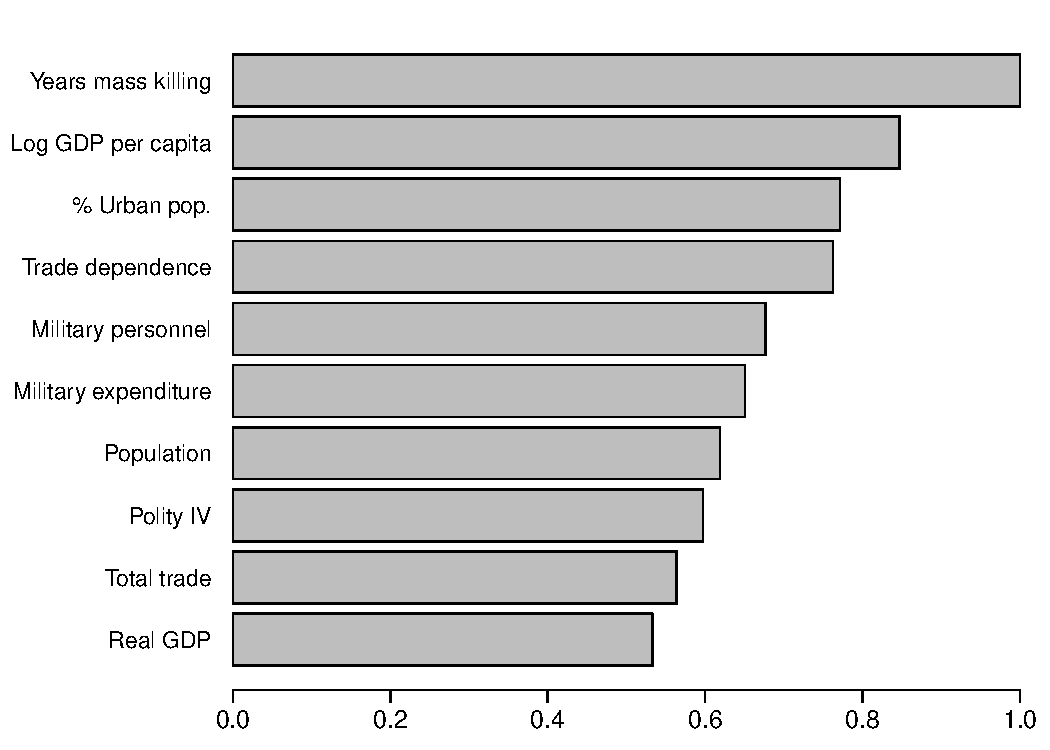
\includegraphics[width=.8\textwidth, height=8.25cm]{images/rf-mk.pdf}
    \caption{Distributed Random Forest -- Variable Importance (Scaled)}
    \label{fig:drfuv}
\end{figure}
	
Interestingly, several variables that are not robust explanators of mass killing in the EBA, have large importance in the machine learning estimates. Variables related to characteristics of the military forces are a good example. As seen below, parametrisation and interactions likely account for this difference. The linear model imposes a parametric structure to the covariate, and the relationship between an independent variable and the response may be a nonlinear one. Also, variables can be relevant predictors only when in interaction with each other. In both cases, those relationships will be captured in the machine learning estimations but not in the extreme bounds analysis. This provides evidence that model specification is driving some of the results in the EBA. 

Figure \ref{fig:drfdpp} displays the partial dependence plots for the ten variables that the distributed random forests highlight as the most important explanators of mass killing onset. These graphs are akin to marginal effect plots in correlation models and help clarify the directional effects of these variables over their entire range. For example, one can see that the effects of Years since Last Mass Killings is highly nonlinear, or that Log GDP per capita does not decrease the likelihood of mass killings after it reaches values close to 9.

\begin{figure}[H]
    \centering
    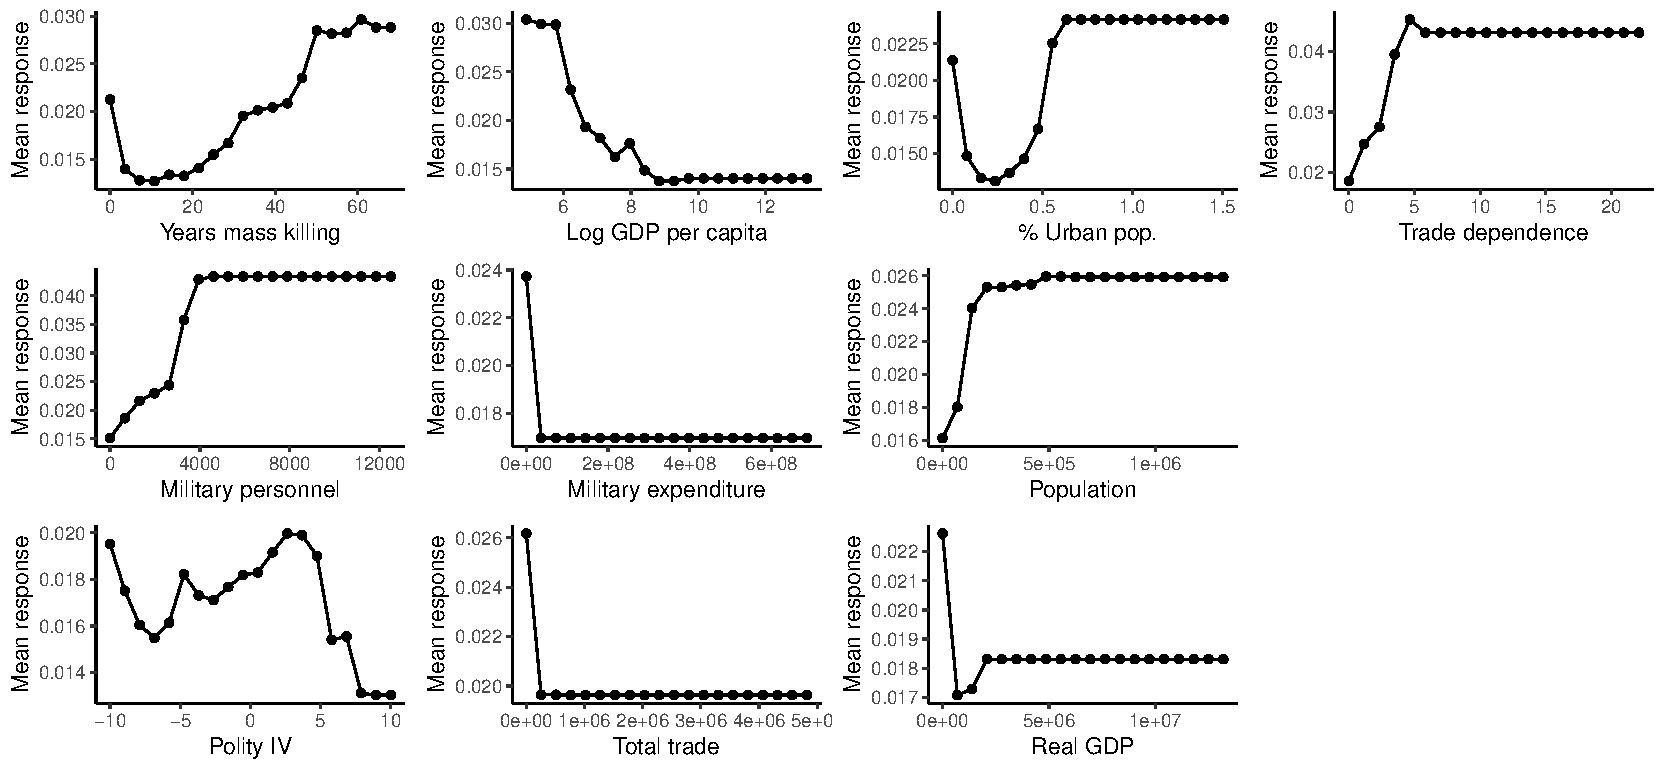
\includegraphics[width=\textwidth, height=8cm]{images/rf-mk-pd.pdf}
    \caption{Distributed Random Forest -- Partial Dependence Plots}
    \label{fig:drfdpp}
\end{figure}

One can also infer that authoritarian and mixed political regimes are more likely to engage in mass violence than democratic countries, a result that is also supported by both the EBA and the specialised literature. The number of military personnel positively affects the likelihood of mass killings, yet this increase is counterbalanced by military expenditures. Taken together, these results indicate that countries with large and poorly-funded armed forces have higher risks of mass violence.

\subsection{Mass Killings during Civil Wars}%
\label{sub:mass_killings_during_civil_wars}

Table \ref{tab:ucdp} presents the EBA results when I restrict the analysis to only civil war years to answer Question 2. I consider three different codings of civil war: 1) the Uppsala Conflict Database Program \citeyear{allansson2017organized,gleditsch2002armed}), 2) the Correlates of War project \citep{sarkees2010resort}, and 3) ethnic civil war from \citet{cederman2010ethnic}. I find two important patterns. First, considering only civil war years provides a very different understanding of atrocity. Across these models, the only similarity with the full analysis is that mass killing is less likely post-Cold War. Instead, military factors, such military size and militias, and territorial war aims are the most robust predictors of atrocity once war begins. However, contrary to past expectation \citep{koren2017means}, militias have a negative impact on the likelihood of mass killings. Second, there is wide variation in which variables are robust depending on how scholars code civil war. Across the three codings I use here, no variable is robust to all codings and only territorial aims and militias are robust to more than one coding. These results are concerning for scholars using correlation models, as they indicate that our understanding of atrocity, from null hypothesis testing, is largely dependent on which coding of civil war researchers use. For example, only the UCDP data suggests that the post-Cold War years see less barbarism than during the Cold War.

\begin{table}[H]
\centering
\begin{tabular}{lrrrrr}
\hline
\textbf{Variable} & \textbf{Avg. $\beta$} & \textbf{Avg. SE} & \textbf{$\%$ Sig.} & \textbf{CDF(0)} & \textbf{Models} \\ \hline
\textit{UCDP Data} &  &  &  &  &  \\
Territory aims & -0.044 & 0.019 & 74.997 & 0.9804 & 17902 \\
Post-Cold War years & -0.038 & 0.019 & 66.574 & 0.9222 & 17902 \\
 &  &  &  &  &  \\
\textit{COW Data} &  &  &  &  &  \\
Physical integrity & 0.024 & 0.013 & 66.674 & 0.9564 & 17902 \\
Militias & -0.099 & 0.048 & 73.104 & 0.9490 & 17902 \\
Years since last mass killing & 0.006 & 0.002 & 88.208 & 0.9472 & 101583 \\
Previous riots & 0.078 & 0.041 & 65.412 & 0.9348 & 17902 \\
Ethnic diversity (ELF) & 0.095 & 0.062 & 48.615 & 0.9000 & 17902 \\
& & & & \\
\textit{Cederman et al. Data} &  &  &  &  &  \\
Territory aims & -0.051 & 0.026 & 74.288 & 0.9167 & 17902 \\
Militias & -0.050 & 0.035 & 52.240 & 0.9101 & 17902 \\ \hline
\end{tabular}
\caption{EBA -- Mass Killings during Civil Wars (Robust Variables Only)}
\label{tab:ucdp}
\end{table}
	
When I analyse the three codings of civil war using random forest analysis, I find further intricacies in the patterns of mass killing. First, the machine learning estimates highlight a different set of variables than the EBA when analysing the UCDP and Ethnic War data. However, the COW EBA and machine learning analyses both highlight the importance of human rights, previous riots, and the time since the state last engaged in mass killing. Thus, the COW analysis provides the most stable picture of atrocity during civil war. It again highlights the important pattern of the Conflict Trap: violence breeds violence. Second, though, the three codings of civil war each highlight a very similar set of strong predictors of atrocity during conflict. Therefore, the machine learning estimates are not as dependent on the data set employed as are the EBA results. This is good news for scholars of mass killing because it indicates that while the parametric models do not produce robust findings across different civil war data sets, the nonlinear models are able to given us a consistent and clear picture of which factors place a country at the greatest risk for atrocity during civil war. 

Figures \ref{fig:drfdpp2}--\ref{fig:drfdpp4} display the partial dependence plots for the variables with the highest impact in each of the three civil war data sets.

\vspace{1cm}
	
\begin{figure}[H]
    \centering
    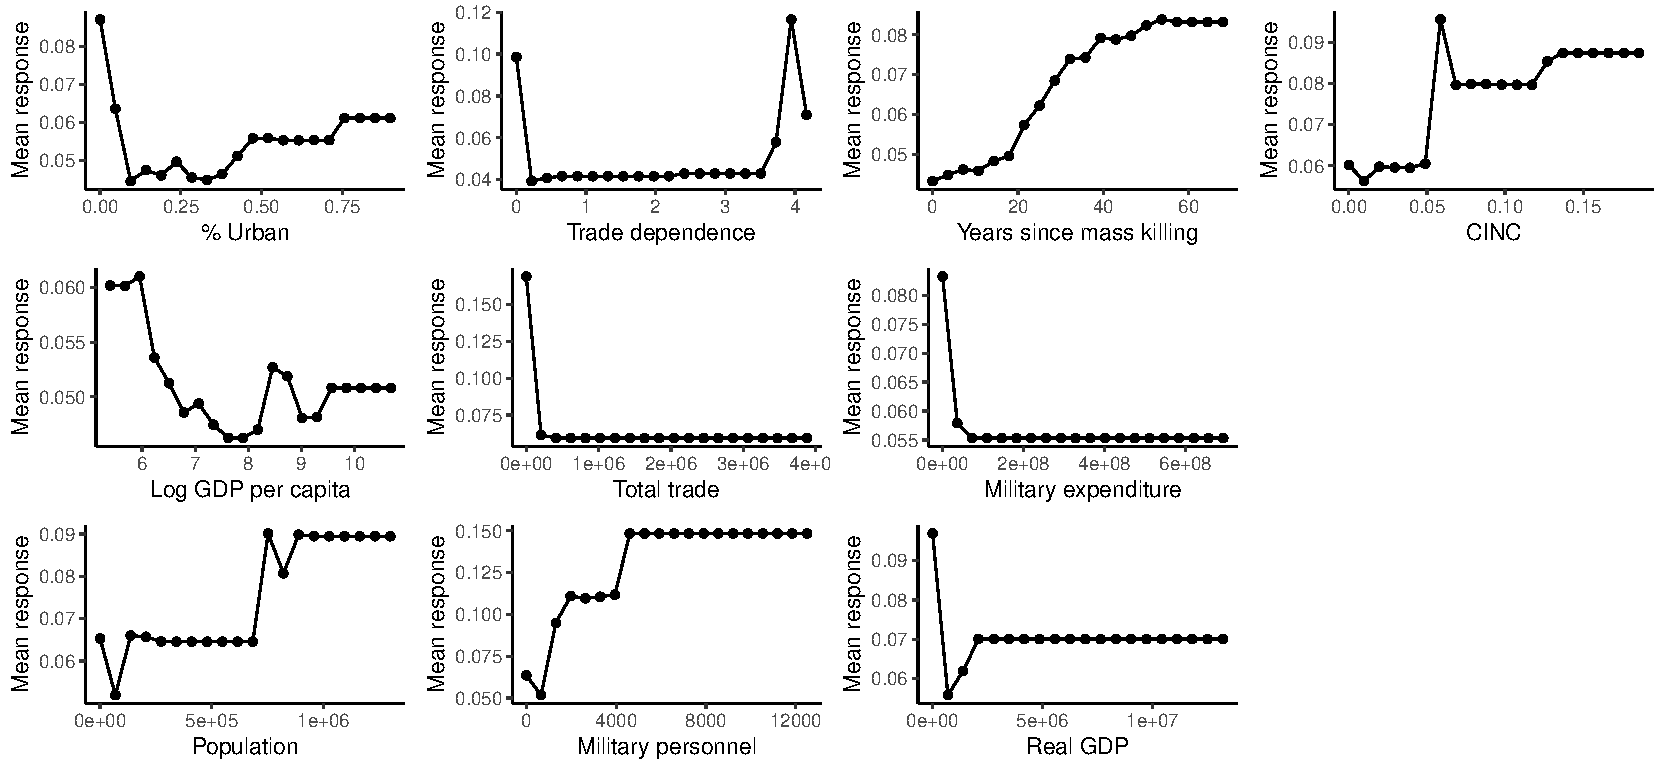
\includegraphics[width=\textwidth, height=8cm]{images/rf-ucdp-pd.pdf}
    \caption{Partial Dependence Plots -- Mass Killings during Civil Wars (UCDP Data)}
    \label{fig:drfdpp2}
\end{figure}
	
\begin{figure}[H]
    \begin{center}
    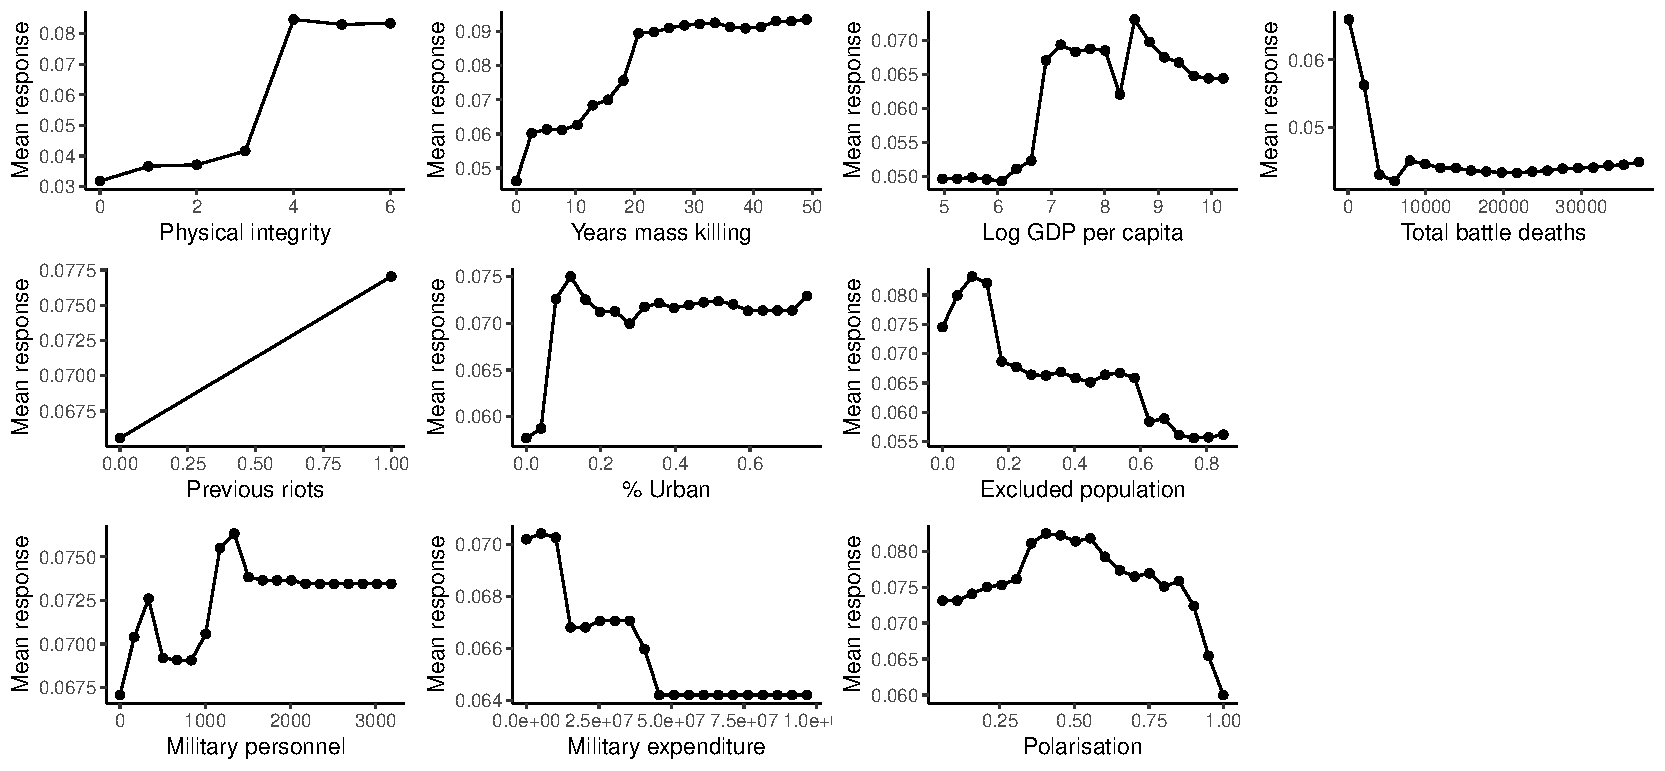
\includegraphics[width=\textwidth, height=8cm]{images/rf-cow-pd.pdf}
    \caption{Partial Dependence Plots -- Mass Killings during Civil Wars (COW Data)}
    \label{fig:drfdpp3}
    \end{center}
\end{figure}	
	
\begin{figure}[H]
    \begin{center}
    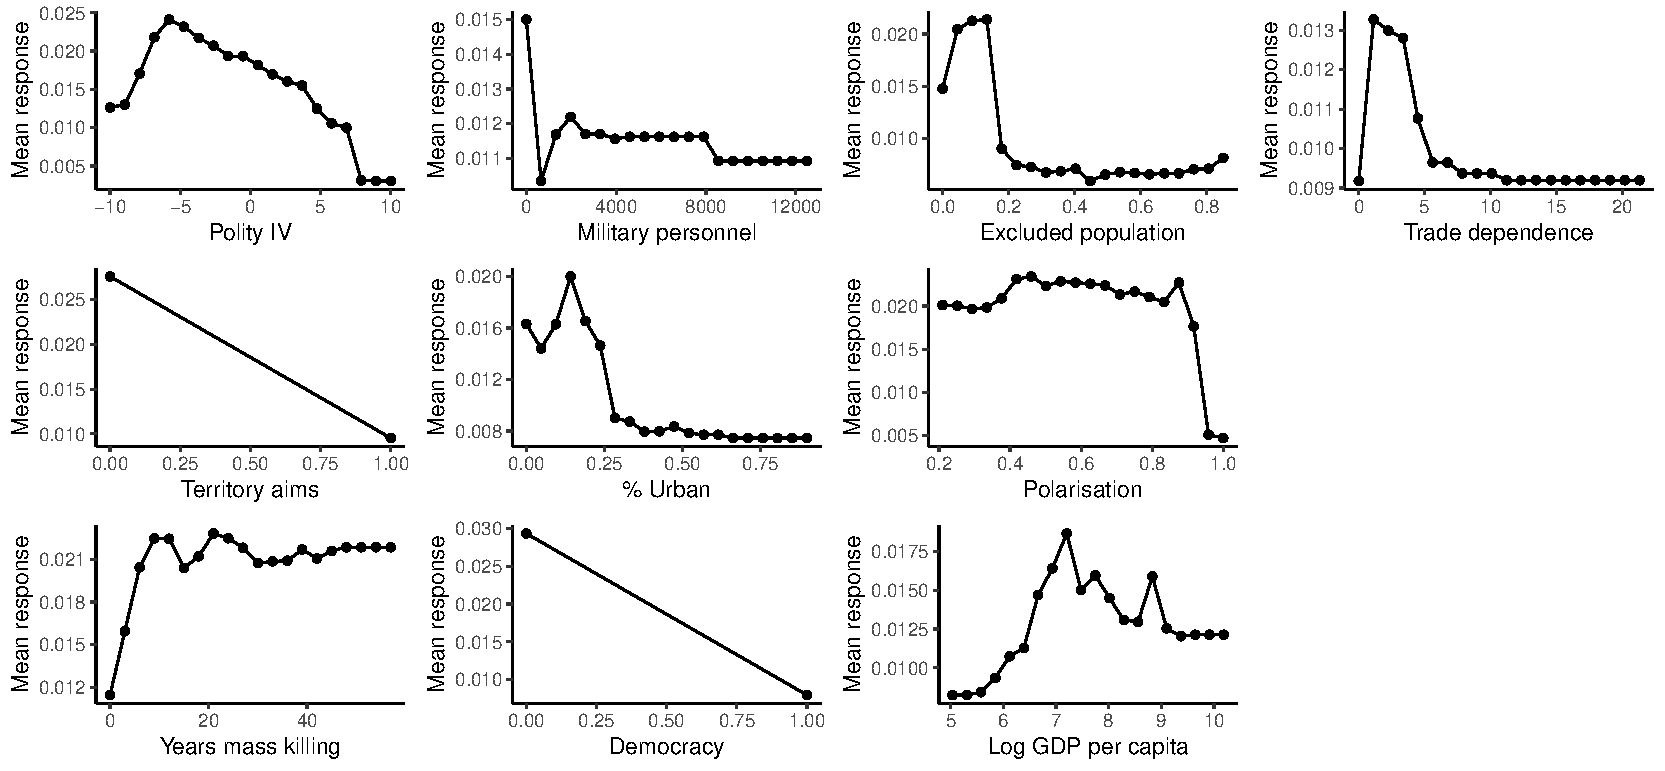
\includegraphics[width=\textwidth, height=8cm]{images/rf-eth-pd.pdf}
    \caption{Partial Dependence Plots -- Mass Killings during Civil Wars (Cederman et al. Data)}
    \label{fig:drfdpp4}
    \end{center}
\end{figure}

\subsection{Mass Killings in and after the Cold War}%
\label{sub:mass_killings_in_and_after_the_cold_war}

Lastly, I test the heterogeneity of the main findings with three sets of models. First, I analyse which factors increase the risk of mass killings during and after the Cold War period. Global dynamics may influence the cost-benefit calculus of state leaders, and consequently affect the likelihood of large-scale responses to internal threats. 

\begin{table}[H]
\centering
\begin{tabular}{lrrrrr}
\hline
\textbf{Variable} & \textbf{Avg. $\beta$} & \textbf{Avg. SE} & \textbf{$\%$ Sig.} & \textbf{CDF(0)} & \textbf{Models} \\ \hline
\textit{Cold War Period} &  &  &  &  &  \\
Log GDP per capita & -0.018 & 0.009 & 83.204 & 0.9678 & 50000 \\
Previous riots & 0.022 & 0.014 & 62.457 & 0.9031 & 8278 \\
 &  &  &  &  &  \\
\textit{Post-Cold War Period} &  &  &  &  &  \\
Ethnic war onset & -0.024 & 0.011 & 89.608 & 0.9823 & 4850 \\
Coup d'état & -0.022 & 0.011 & 89.200 & 0.9822 & 8602 \\ 
Territory aims & -0.027 & 0.014 & 81.083 & 0.9653 & 8775 \\ 
Displaced Population & -0.048 & 0.027 & 58.689 & 0.9392 & 8695 \\ \hline
\end{tabular}
\caption{EBA -- Mass Killings in and after the Cold War Period (Robust Variables Only)}
\label{tab:coldwar}
\end{table}

The EBA models show different patterns for both periods. In the Cold War years, Log GDP per capita has a negative impact on mass killings, while instances of previous riots increase the likelihood of state-led atrocities. The results are in line with those of the pooled model. However, mass killings seem to follow a separate logic in the post-Cold War years. Four independent variables lower the risk of mass killings: ethnic war onset, wars fought for territorial aims, coups d'état, and the share of discriminated population. I interpret the results as showing that ethnic wars are fought by groups with similar capabilities, thus large-scale, one-sided violence is relatively rare. This also explains why atrocities are more likely to occur in countries where the share of discriminated population is not very large. The models show that territorial wars lead to more mass killings than governmental conflicts, a findings which has been previously described in the literature \citep[240]{eck2007one}. Coups d'état are correlated with fewer atrocities as well, what stands in contrast with previous research \citep[10]{wayman2010explaining}.

The random forests models also display some difference between the two periods, yet several variables appear in both estimations and in the main models presented above. The results for the Cold War model also classify Log GDP per capita and previous riots as important predictors of mass killings. As expected, the effect is negative for income and positive for past social upheavals. The variables that appear in the main model have similar distribution, such as the inverted-U relationship between the Polity IV index and mass killings, and the shape decline in atrocity risk when Log GDP per capita has a value of of 10. 

\begin{figure}[H]
    \centering
    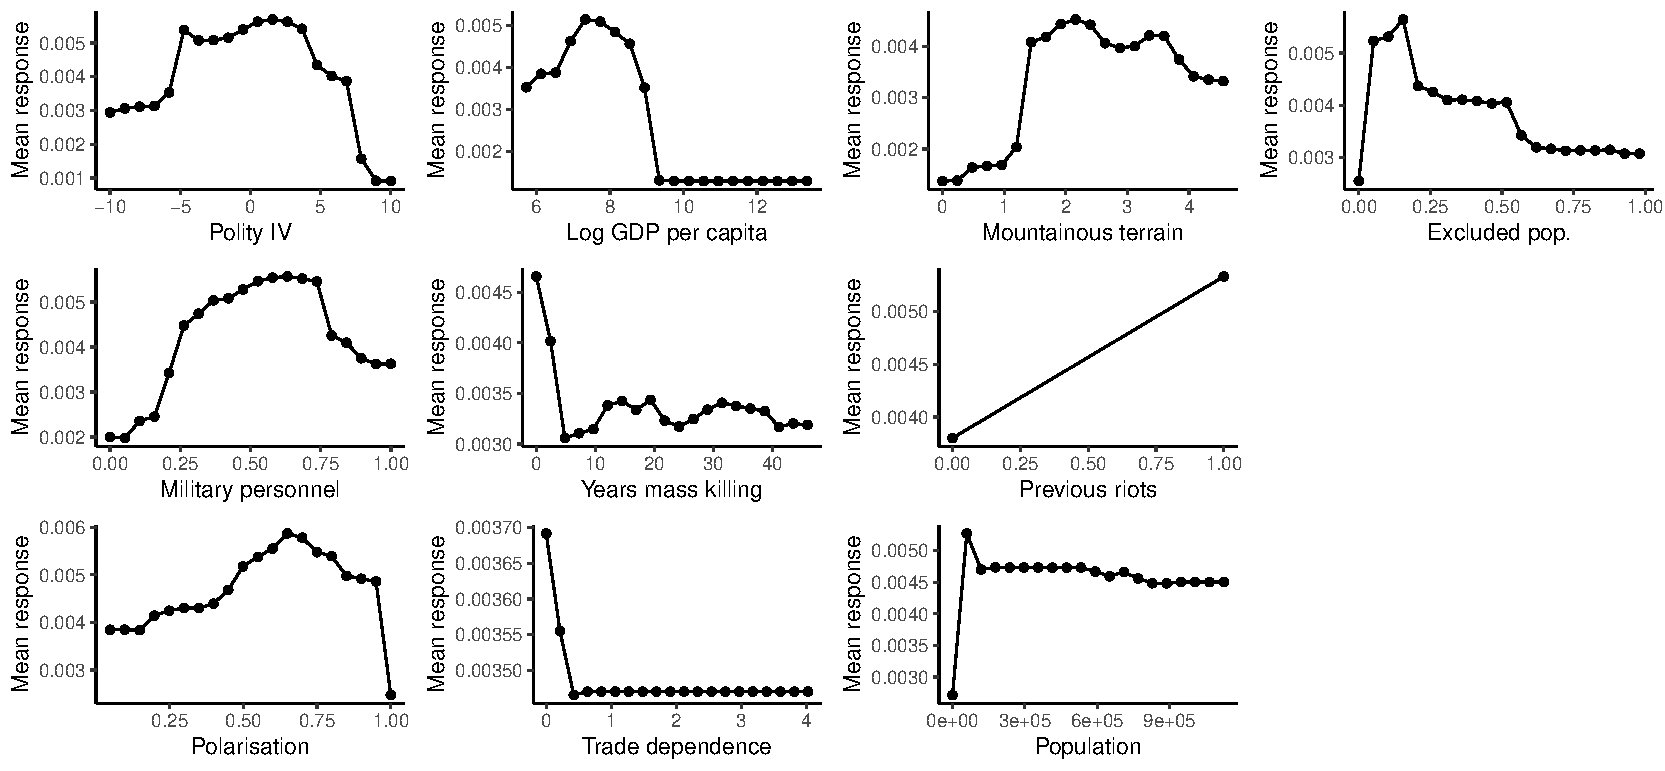
\includegraphics[width=\textwidth, height=8cm]{images/rf-coldwar-pd.pdf}
    \caption{Partial Dependence Plots -- Mass Killings during the Cold War Period}
    \label{fig:drfdpp2}
\end{figure}
	
\begin{figure}[H]
    \begin{center}
    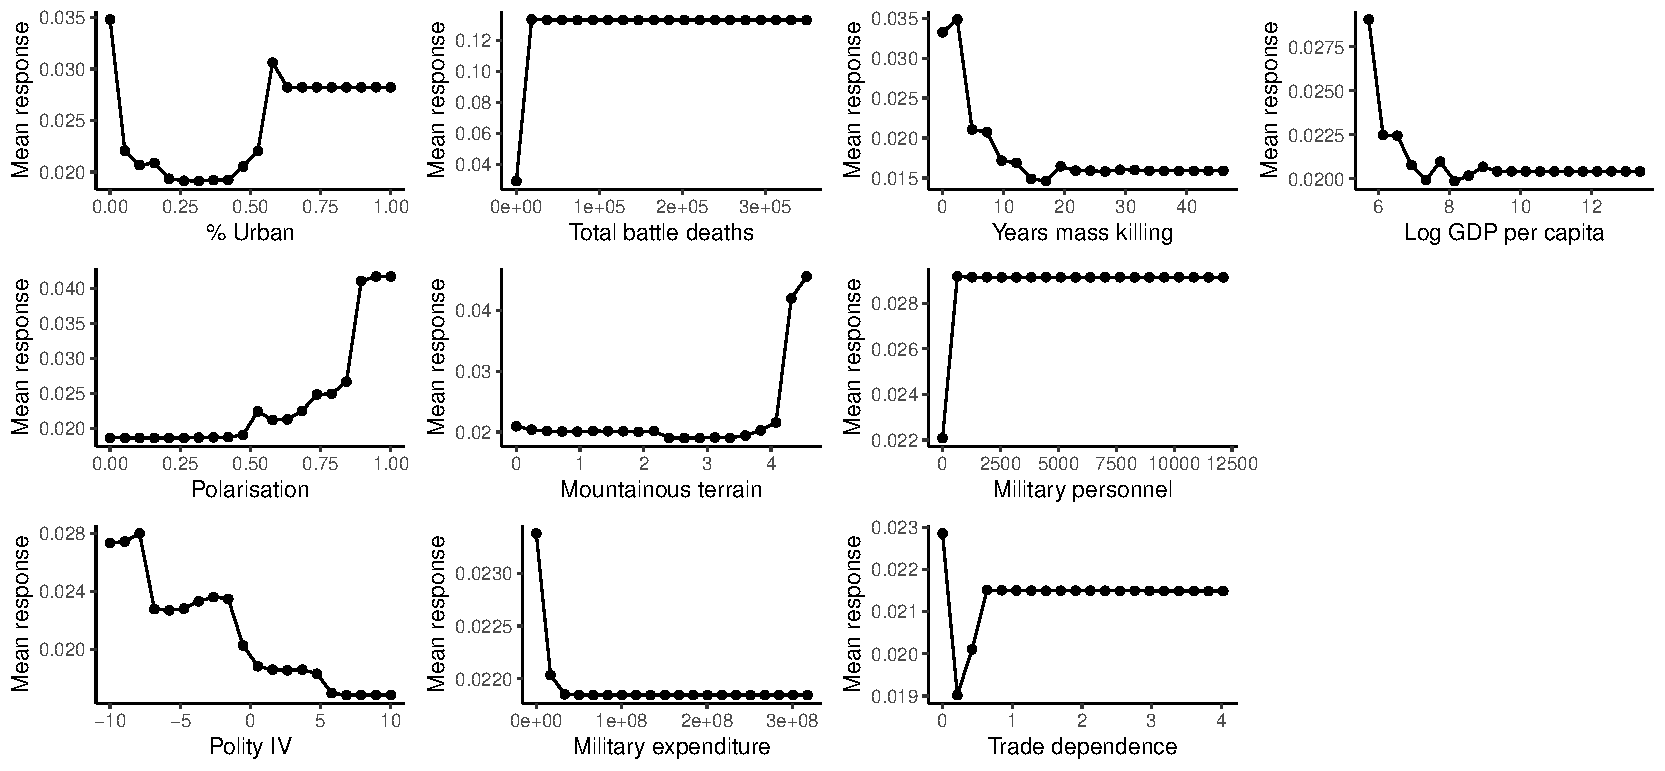
\includegraphics[width=\textwidth, height=8cm]{images/rf-postcoldwar-pd.pdf}
    \caption{Partial Dependence Plots -- Mass Killings after the Cold War Period}
    \label{fig:drfdpp3}
    \end{center}
\end{figure}	

\subsection{Genocides and Politicides}%
\label{sub:genocides_and_politicides}

To answer Question 3, I estimate the same regressions using Harff's (\citeyear{harff2003no}) indicator of genocide and politicide. No variable appears significant in the EBA models for genocide or politicide onset in the full data set. When I limit the sample to civil war years, the Post-Cold War period is negatively correlated with the outcome when using the Correlates of War data set. Excluded population has a negative sign in more than 90\% of the models using both Correlates of War's and Cederman et al's (\citeyear{cederman2010ethnic}) indicators of conflict. Displaced population also has a negative effect in the Correlates of War data set. During ethnic conflicts, the dummy variable for political assassinations has a negative impact on the onset of genocides. Overall, from these EBA analyses, one can conclude then that the significant covariates of genocide and politicide onset differ significantly from those of more general forms of government mass violence. Though, the opportunity story still receives some limited support in these models. However, the machine learning models using Harff's genocide and politicide data are comparable to the ones I present above, with a similar set of variables appearing in the random forest estimations. These results once more highlight that while the mass killing literature struggles to identify correlates of atrocity that are robust across model specification, scholars have done a much better job at identifying variables that help predict both the onset of genocide/politicide and mass killings, more broadly.

\section{Additional Tests}
\label{sec:additional-tests4}

I estimate a set of additional regressions to assess the robustness of the main findings.\footnote{For computational purposes, I conducted all additional tests on 50,000 random draws from EBA's posterior distribution. \citet[819]{salaimartin2004determinants} argue that random draws from the full EBA models are unbiased.} In regard to EBA, I include 10 variants of the original model. They largely confirm the prior results. First, I varied the number of covariates included in each regression to 3 and 5 while keeping the $M$ set of 3 control variables. The results are the same as those of the main model, except that ethnic fractionalisation and Polity IV squared become marginally significant with a CDF(0) of about 0.88. Second, I place different restrictions on the variance inflation factor (VIF) to test whether multicollinearity is driving the results. The two models with different values of VIF are identical to the model reported here, while in the model with no VIF restriction ethnic fractionalisation again fails to meet the threshold by a very small margin. 
	
I also reestimate the models using logit and probit regressions. In order to deal with the issue of complete separation \citep{bell2015questioning,zorn2005solution} I follow \citet{gelman2008weakly} and add a weakly informative prior distribution to the coefficients. In both cases, the logarithm of GDP per capita, post-Cold War period, previous riots, and Polity IV squared remain significant.

As a last robustness test for the EBA, I ran the main model with peace years only; that is, only country-years in which the UCDP, COW and Cederman et al's dichotomous measures of civil conflicts are equal to zero. Despite some issues of multicollinearity,\footnote{Some independent variables were dropped from the models due to problems of collinearity. The bounds for my indicator of ``wars fought over territory'' could not be estimated, and the coefficients for ``number of battle deaths'' and ``presence of guerrillas'' are unreliable due to their sample sample size. The appendix contains the distribution of the coefficients.} the results are similar to the original model, what indicates that the difference in the estimations is conditional on civil war years.
	
In regard to random forests, grid searches are themselves a data-driven selection of many possible machine learning models, thus it is not strictly necessary to run a batch of additional tests. Nevertheless, I performed a series of grid searches using three different seeds obtained from \href{https://random.org}{\texttt{http://random.org}} to estimate how different starting numbers influence the model outcomes. The output of those models are largely comparable. The results of each of these analyses are available in the appendix.

\section{Conclusion}
\label{sec:conclusion}
	
In this chapter, I apply extreme bounds analysis and distributed random forests to estimate the robustness and predictive ability of 40 variables that have been pointed out as potential determinants of mass killings. I find strong evidence that mass killings are unlikely to happen in rich, stable countries. Nevertheless, there is considerable heterogeneity in some of the results. The findings point out that mass killings have different causes according to the context in which they erupt, so a general theory of state atrocities may obscure important details in our understanding of state killings. Moreover, mass killings are rare events, so local factors likely play an important role in their onset \citep{straus2007second,straus2012destroy}.
	
Yet one can see this diversity of outcomes under a positive light. The results above suggest new avenues for research, and they also highlight the importance of scholars moving from simple cross-country regressions to methods that can yield more robust predictions. For instance, why are mass killings in ethnic conflicts correlated with a different set of variables than in armed conflicts in general? Would the results remain robust had scholars decided to code ethnic conflicts in another way? More theoretical advancement would also be welcome. Given that GDP per capita is negatively correlated to state atrocities in virtually every model, it would be interesting to unpack the causal mechanisms by which it operates by testing more specific mechanisms. 
	
In terms of practical implications, the results indicate that democratisation and pro-growth economic policies are the most efficient ways to prevent mass killings. The international community can therefore play a role in deterring leaders from using force against their own population, either by offering support for domestic opposition groups, intervening, or by fostering economic development. Although costly in the short run, and sometimes violent during the transition, these measures would substantially decrease the likelihood of state violence by breaking the ``conflict trap'' in which past conflicts create the condition for new ones \citep{collier2003breaking}.

\newpage

\section{Appendix} 
\label{sec:mk-appendix}

This appendix contains all required information to replicate the numerical analyses presented in sections \ref{sec:results4} and \ref{sec:additional-tests4}. \textt{R} code can be found in subsection \ref{sec:mk-code} and the data are available on the following GitHub repository: \href{https://github.com/danilofreire/mass-killings}{https://github.com/danilofreire/mass-killings}. I used \texttt{R} version 3.4.4 (15-03-2018) and Ubuntu 16.04.4 LTS to perform all statistical calculations.

\subsection{Variable Selection}
\label{sec:mk-vs}

I employ some criteria to select our explanatory variables. First, I included only published articles in the sample. Although working papers and policy may also provide important insights about the onset of mass killings, peer-reviewed research is probably better suited for our purposes. Also, I included only papers that use regression methods on a global sample and were published from 1995 to 2015. The final sample comprises 45 articles: \citet{anderton2015new}, \citet{balcells2010rivalry, balcells2011continuation}, \citet{besanccon2005relative}, \citet{bulutgil2015social}, \citet{bundervoet2009livestock}, \citet{clayton2016civilianizing}, \citet{colaresi2008kill}, \citet{downes2006desperate, downes2007restraint},  \citet{easterly2006development}, \citet{eck2007one}, \citet{esteban2015strategic}, \citet{fazal2015particular}, \citet{fjelde2014weakening}, \citet{goldsmith2013forecasting}, \citet{harff2003no}, \citet{joshi2017kills}, \citet{kim2010makes}, \citet{kim2016revolutionary}, \citet{kisangani2007political}, \citet{koren2017means}, \citet{krain1997state}, \citet{manekin2013violence}, \citet{mcdoom2013killed,mcdoom2014predicting}, \citet{melander2009new}, \citet{montalvo2008discrete}, \citet{pilster2016differentiation}, \citet{querido2009state}, \citet{raleigh2012violence}, \citet{rost2013will}, \citet{rummel1995democracy}, \citet{schneider2013accounting}, \citet{siroky2015empire}, \citet{stanton2015regulating}, \citet{sullivan2012blood}, \citet{tir2008domestic}, \citet{ulfelder2008assessing}, \citet{ulfelder2012forecasting}, \citet{uzonyi2015civil, uzonyi2016domestic} \citet{valentino2004draining}, \citet{valentino2006covenants}, \citet{verpoorten2012leave}, \citet{wayman2010explaining}, \citet{wig2016local}, and \citet{yanagizawa2014propaganda}.

In those 45 studies, scholars made use of nearly 180 measurements to capture roughly 30 key concepts related to threat and costs of mass killings. To be added to our models, a variable should appear in at least two articles. The covariates are summarised in table \ref{tab:mk-vs}. A complete list of variables is available at \href{https://github.com/danilofreire/mass-killings}{https://github.com/danilofreire/mass-killings}.


\begin{table}[!htbp] \centering 
  \caption{Independent Variables} 
  \label{tab:mk-vs} 
\footnotesize
\begin{tabular}{@{\extracolsep{5pt}}lcc} 
\\[-1.8ex]\hline 
\hline \\[-1.8ex] {Variable} & \multicolumn{1}{c}{Coded} & \multicolumn{1}{c}{Source}\\ 
\hline \\[-1.8ex] 
Assassination & Dichotomous & \citet{banks1999cross} \\ 
CINC & Continuous & \citet{cow2017cinc}\\ 
Coup d'état & Dichotomous & \citet{marshall2017pitf}  \\ 
COW civil war onset & Dichotomous & \citet{cow2017cinc,singer1988reconstructing} \\ 
COW civil war ongoing & Dichotomous & \citet{cow2017cinc,singer1988reconstructing} \\ 
Democracy (Polity IV $\geq 6$) & Dichotomous  & Authors' own calculations \\ 
Discriminated dummy & Dichotomous & \citet{cederman2010ethnic}\\ 
Discriminated population & Continuous & \citet{cederman2010ethnic} \\ 
Ethnic diversity (ELF) & Continuous & \citet{fearon2003ethnicity} \\ 
Ethnic war start & Dichotomous & \citet{cederman2010ethnic} \\ 
Ethnic war ongoing & Dichotomous & \citet{cederman2010ethnic} \\ 
Excluded population & Continuous & \citet{cederman2010ethnic} \\ 
Interstate war & Dichotomous & \citet{singer1988reconstructing,cow2017cinc} \\ 
Guerrilla & Dichotomous & \citet{balcells2014does}\\ 
Military expenditure & Continuous & \citet{cow2017cinc} \\ 
Military personnel & Continuous & \citet{cow2017cinc} \\ 
Militias & Dichotomous & \citet{carey2013states} \\ 
Mountainous Terrain & Continuous & \citet{fearon2003ethnicity} \\ 
Physical integrity & Continuous & \citet{cingranelli2010cingranelli}\\ 
Polarisation (all groups/main group) & Continuous &  Authors' own calculations \\ 
Polarisation (all groups/population) & Continuous &  Authors' own calculations  \\ 
Polarisation (included groups/population) & Continuous &  Authors' own calculations  \\ 
Polarisation (included groups/main group) & Continuous &  Authors' own calculations  \\ 
Polity IV & Continuous & \citet{marshall2017pitf}\\ 
Polity IV squared & Continuous & Authors' own calculations \\ 
Population & Continuous & \citet{gleditsch2002expanded} \\
Post-Cold War & Dichotomous & Authors' own calculations \\ 
Real GDP & Continuous & \citet{gleditsch2002expanded} \\ 
Real GDP per capita & Continuous & \citet{gleditsch2002expanded} \\ 
Real GDP per capita (log) & Continuous & Authors' own calculations  \\ 
Regime transition & Continuous & Authors' own calculations \\ 
Riot & Dichotomous & \citet{banks1999cross}\\ 
Total battle deaths & Continuous & \citet{lacina2005monitoring} \\  
Total trade & Continuous & \citet{cow2017cinc} \\ 
Trade dependence (total trade/real GDP) & Continuous & Authors' own calculations \\ 
UCDP civil war onset & Dichotomous & \citet{allansson2017organized,gleditsch2002armed} \\ 
UCDP civil war ongoing & Dichotomous & \citet{allansson2017organized,gleditsch2002armed} \\ 
Urban population (percentage) & Continuous & \citet{cow2017cinc} \\ 
Years since last mass killing & Continuous & Authors' own calculations \\ 
War with territory aims & Dichotomous & \citet{allansson2017organized,gleditsch2002armed} \\ 
\hline \\[-1.8ex] 
\end{tabular} 
\end{table} 

\newpage

\subsection{Descriptive Statistics}
\label{sec:mk-ds}

\begin{table}[!htbp] \centering 
  \caption{Descriptive Statistics} 
  \label{tab:mk-ds} 
\footnotesize 
\begin{tabular}{@{\extracolsep{5pt}}lccccc} 
\\[-1.8ex]\hline 
\hline \\[-1.8ex] 
Statistic & \multicolumn{1}{c}{N} & \multicolumn{1}{c}{Mean} & \multicolumn{1}{c}{St. Dev.} & \multicolumn{1}{c}{Min} & \multicolumn{1}{c}{Max} \\ 
\hline \\[-1.8ex] 
Country code & 9,162 & 452.84 & 247.74 & 2 & 950 \\ 
Year & 9,162 & 1,983.56 & 18.77 & 1,945 & 2,013 \\ 
Genocide/politicide onset & 8,933 & 0.005 & 0.07 & 0 & 1\\ 
Mass killing onset & 9,162 & 0.01 & 0.11 & 0 & 1 \\ 
&&&&&\\
\textit{Independent Variables} & & & & \\
&&&&&\\
Assassination dummy & 8,991 & 0.08 & 0.27 & 0 & 1 \\ 
CINC & 8,767 & 0.01 & 0.02 & 0.00 & 0.38 \\ 
Coup dummy & 8,587 & 0.05 & 0.21 & 0 & 1 \\ 
COW civil war onset & 8,160 & 0.01 & 0.12 & 0 & 1 \\ 
COW civil war ongoing & 8,160 & 0.07 & 0.25 & 0 & 1 \\ 
Democracy dummy & 8,991 & 0.37 & 0.48 & 0 & 1 \\ 
Discriminated dummy & 6,981 & 0.35 & 0.48 & 0 & 1 \\ 
Discriminated population & 6,981 & 0.06 & 0.15 & 0.00 & 0.98 \\ 
Ethnic diversity (ELF) & 6,981 & 0.41 & 0.31 & 0 & 1 \\ 
Ethnic war start & 7,760 & 0.01 & 0.12 & 0 & 1 \\ 
Ethnic war ongoing & 7,760 & 0.11 & 0.31 & 0 & 1 \\ 
Excluded population & 6,981 & 0.16 & 0.22 & 0.00 & 0.98 \\ 
Interstate war & 8,159 & 0.04 & 0.19 & 0 & 1 \\ 
Guerrilla dummy & 714 & 0.81 & 0.40 & 0 & 1 \\ 
Military expenditure & 8,290 & 4,607,120 & 27,785,906 & 0 & 693,600,000 \\ 
Military personnel & 8,620 & 176.70 & 520.90 & 0 & 12,500 \\ 
Militias & 4,097 & 0.22 & 0.42 & 0 & 1 \\ 
Mountainous Terrain & 7,358 & 2.14 & 1.43 & 0.00 & 4.56 \\ 
Physical integrity & 4,499 & 4.73 & 2.31 & 0 & 8 \\ 
Polarisation (all groups/main group) & 6,981 & 0.70 & 0.26 & 0.05 & 1 \\ 
Polarisation (all groups/population) & 6,981 & 0.63 & 0.32 & 0 & 1 \\ 
Polarisation (included groups/population) & 5,610 & 0.64 & 0.32 & 0 & 1 \\ 
Polarisation (included groups/main group) & 6,981 & 0.23 & 0.35 & 0 & 1 \\ 
Polity IV & 8,558 & 0.42 & 7.50 & $-$10 & 10 \\ 
Polity IV squared & 8,558 & 56.35 & 32.59 & 0 & 100 \\ 
Population & 8,293 & 32,993.61 & 112,886.40 & 118.21 & 1,324,353.00 \\
Post-Cold War & 8,991 & 0.40 & 0.49 & 0 & 1 \\ 
Real GDP & 8,293 & 215,317.70 & 804,827.20 & 129.68 & 13,193,478.00 \\ 
Real GDP per capita & 8,293 & 8,104.20 & 18,376.73 & 132.82 & 632,239.50 \\ 
Real GDP per capita (log) & 8,293 & 8.25 & 1.20 & 4.89 & 13.36 \\ 
Regime transition & 1,221 & $-$4.24 & 41.50 & $-$77 & 99 \\ 
Riot dummy & 8,991 & 0.16 & 0.36 & 0 & 1 \\ 
Total battle deaths & 714 & 6,050.86 & 24,404.78 & 100 & 350,000 \\  
Total trade & 8,174 & 53,804.01 & 222,209.90 & 0.80 & 4,825,363.00 \\ 
Trade dependence & 7,670 & 0.26 & 0.69 & 0.0001 & 22.11 \\ 
UCDP civil war onset & 8,733 & 0.02 & 0.14 & 0 & 1 \\ 
UCDP civil war ongoing & 8,733 & 0.15 & 0.36 & 0 & 1 \\ 
Urban population (percentage) & 8,767 & 0.22 & 0.17 & 0.00 & 1.51 \\ 
Years since last mass killing & 9,162 & 23.81 & 17.71 & 0 & 68 \\ 
War with territory aims & 8,924 & 0.07 & 0.26 & 0 & 1 \\ 
\hline \\[-1.8ex] 
\end{tabular} 
\raggedright{\newline \textit{Note}: All independent variables were lagged one year.}
\end{table} 
\normalsize

\newpage

\subsection{Extreme Bounds Analysis Extensions}
\label{sec:mk-ebae}

\subsubsection{Main Model}

I present a series of histograms with the coefficients' distribution of all variables in the main EBA model. There are 36 variables in total, seven of which are robust: Log GDP per capita, post-Cold War period, onset and ongoing civil wars (measured by the UCDP), previous riots, ethnic diversity and the squared term of the Polity IV index.

\vspace{1cm}

\begin{table}[H]
\centering
\begin{tabular}{lrrrrr}
\hline
\textbf{Variable} & \textbf{Avg. $\beta$} & \textbf{Avg. SE} & \textbf{$\%$ Sig.} & \textbf{CDF(0)} & \textbf{Models} \\ \hline
\textit{Base variables} &  &  &  &  &  \\
Log GDP per capita & -0.0091 & 0.0052 & 76.055 & 0.9335 & 226707 \\
 &  &  &  &  &  \\
\textit{Additional variables} &  &  &  &  &  \\
Post-Cold War years & -0.0133 & 0.0085 & 72.845 & 0.9472 & 35614 \\
UCDP civil war onset & 0.0529 & 0.0321 & 52.378 & 0.9441 & 20854 \\
Previous riots & 0.0140 & 0.0100 & 56.242 & 0.9216 & 35614 \\
UCDP ongoing civil war & 0.0172 & 0.0115 & 65.652 & 0.9092 & 20854 \\
Ethnic diversity (ELF) & 0.0184 & 0.0137 & 56.674 & 0.9050 & 35614 \\
Polity IV squared & -0.0002 & 0.0001 & 61.206 & 0.9031 & 35614 \\ \hline
\end{tabular}
\caption{Extreme Bounds Analysis -- Mass killings}
\label{tab:mk}
\end{table}

\clearpage
\begin{sidewaysfigure}
    \centering
    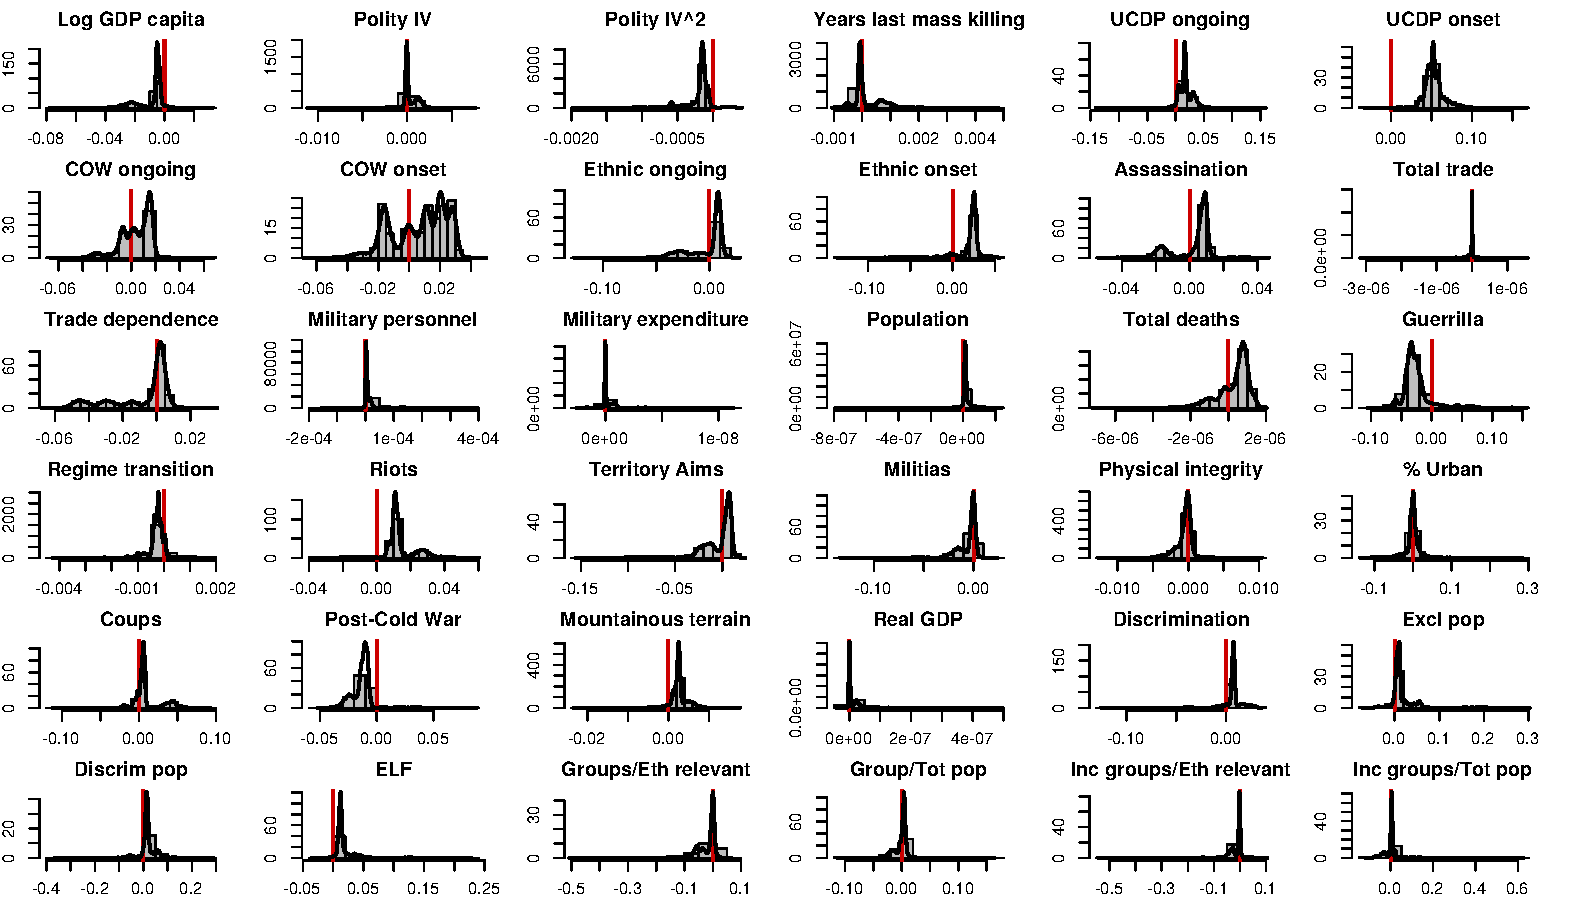
\includegraphics[width=\textwidth]{images/mk.pdf}
    \caption{Extreme Bounds Analysis -- Mass Killings}
    \label{fig:mk}
\end{sidewaysfigure}
\clearpage

\subsubsection{Genocides during Civil Wars}
\label{sec:civil-wars}

Next, I discuss genocides that occur during wartime. I use three covariates that denote ongoing civil conflicts: one by the Uppsala Conflict Data Program \citep{allansson2017organized,gleditsch2002armed}, another by the Correlates of War \citep{sarkees2010resort}, and a third indicating the onset of ethnic conflict as coded by \citet{cederman2010ethnic}. The variables that reach significance in this set of models below are notably different from those obtained in the main estimation. This result provides evidence that mass violence during wartime time follows a separate logic from state killings in peacetime.

\vspace{1cm}

\begin{table}[H]
\centering
\begin{tabular}{lrrrrr}
\hline
\textbf{Variable} & \textbf{Avg. $\beta$} & \textbf{Avg. SE} & \textbf{$\%$ Sig.} & \textbf{CDF(0)} & \textbf{Models} \\ \hline
\textit{UCDP data} &  &  &  &  &  \\
Territory aims & -0.044 & 0.019 & 74.997 & 0.9804 & 17902 \\
Post-Cold War years & -0.038 & 0.019 & 66.574 & 0.9222 & 17902 \\
 &  &  &  &  &  \\
\textit{COW data} &  &  &  &  &  \\
Physical integrity & 0.024 & 0.013 & 66.674 & 0.9564 & 17902 \\
Militias & -0.099 & 0.048 & 73.104 & 0.9490 & 17902 \\
Years since last mass killing & 0.006 & 0.002 & 88.208 & 0.9472 & 101583 \\
Previous riots & 0.078 & 0.041 & 65.412 & 0.9348 & 17902 \\
Ethnic diversity (ELF) & 0.095 & 0.062 & 48.615 & 0.9000 & 17902 \\
 &  &  &  &  &  \\
\textit{Cederman et al. data} &  &  &  &  &  \\
Territory aims & -0.051 & 0.026 & 74.288 & 0.9167 & 17902 \\
Militias & -0.050 & 0.035 & 52.240 & 0.9101 & 17902 \\ \hline
\end{tabular}
\caption{EBA -- Mass Killings during Civil Wars}
\label{tab:ucdp1}
\end{table}

\clearpage
\begin{sidewaysfigure}
    \centering
    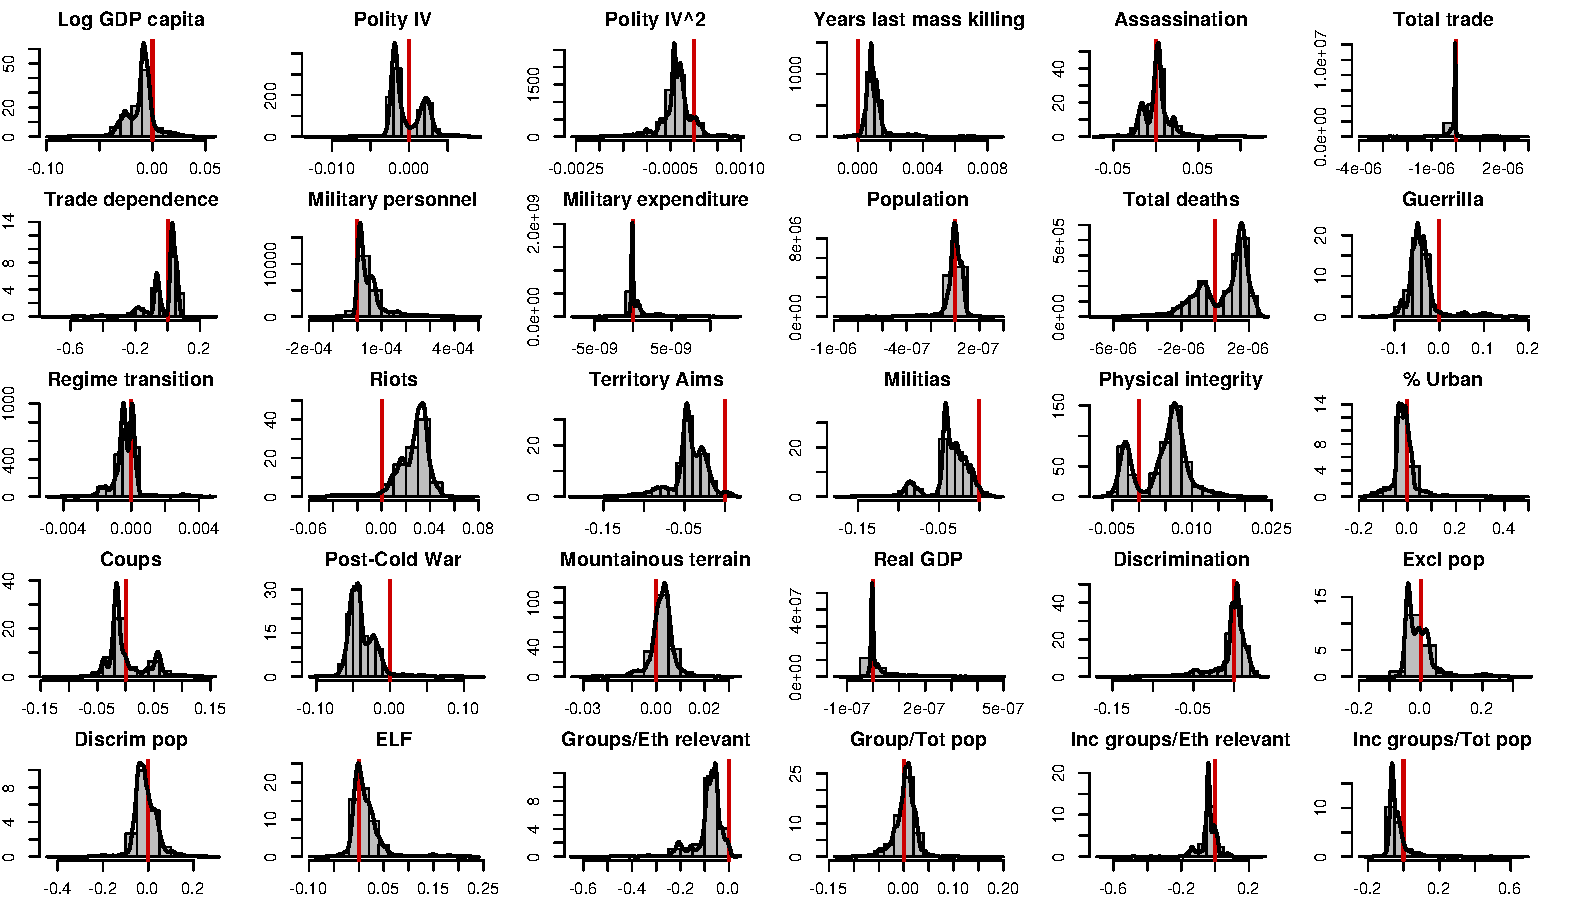
\includegraphics[width=\textwidth]{images/mk-ucdp.pdf}
    \caption{EBA -- Mass Killings during Civil Wars (UCDP Data)}
    \label{fig:mk-ucdp}
\end{sidewaysfigure}
\clearpage

\clearpage
\begin{sidewaysfigure}
    \centering
    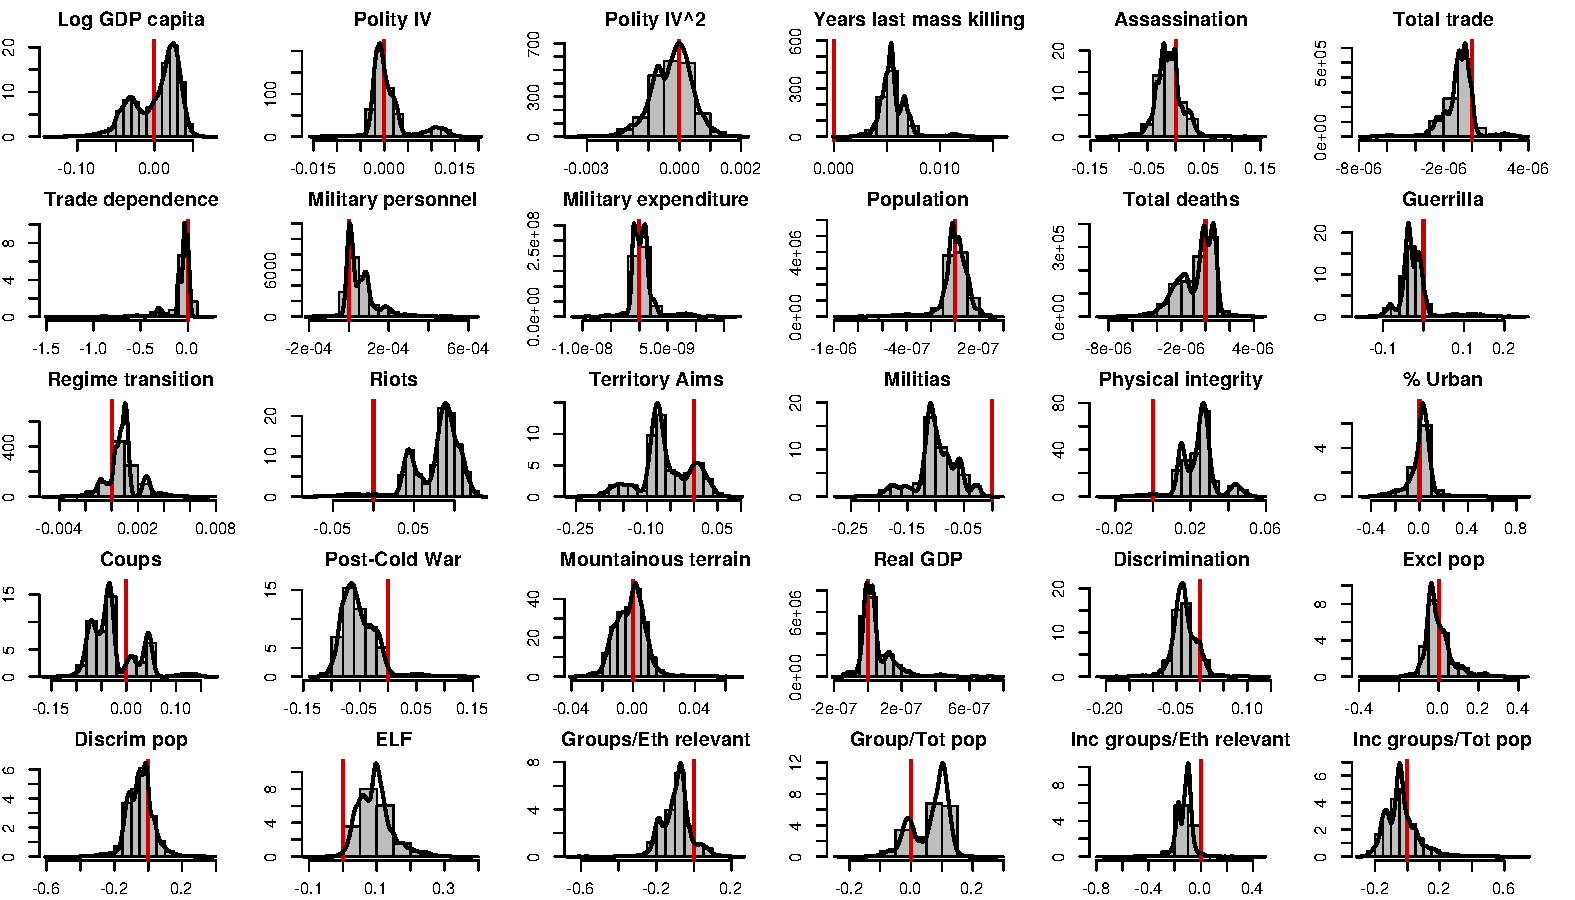
\includegraphics[width=\textwidth]{images/mk-cow.pdf}
    \caption{EBA -- Mass Killings during Civil Wars (COW Data)}
    \label{fig:mk-cow}
\end{sidewaysfigure}
\clearpage

\clearpage
\begin{sidewaysfigure}
    \centering
    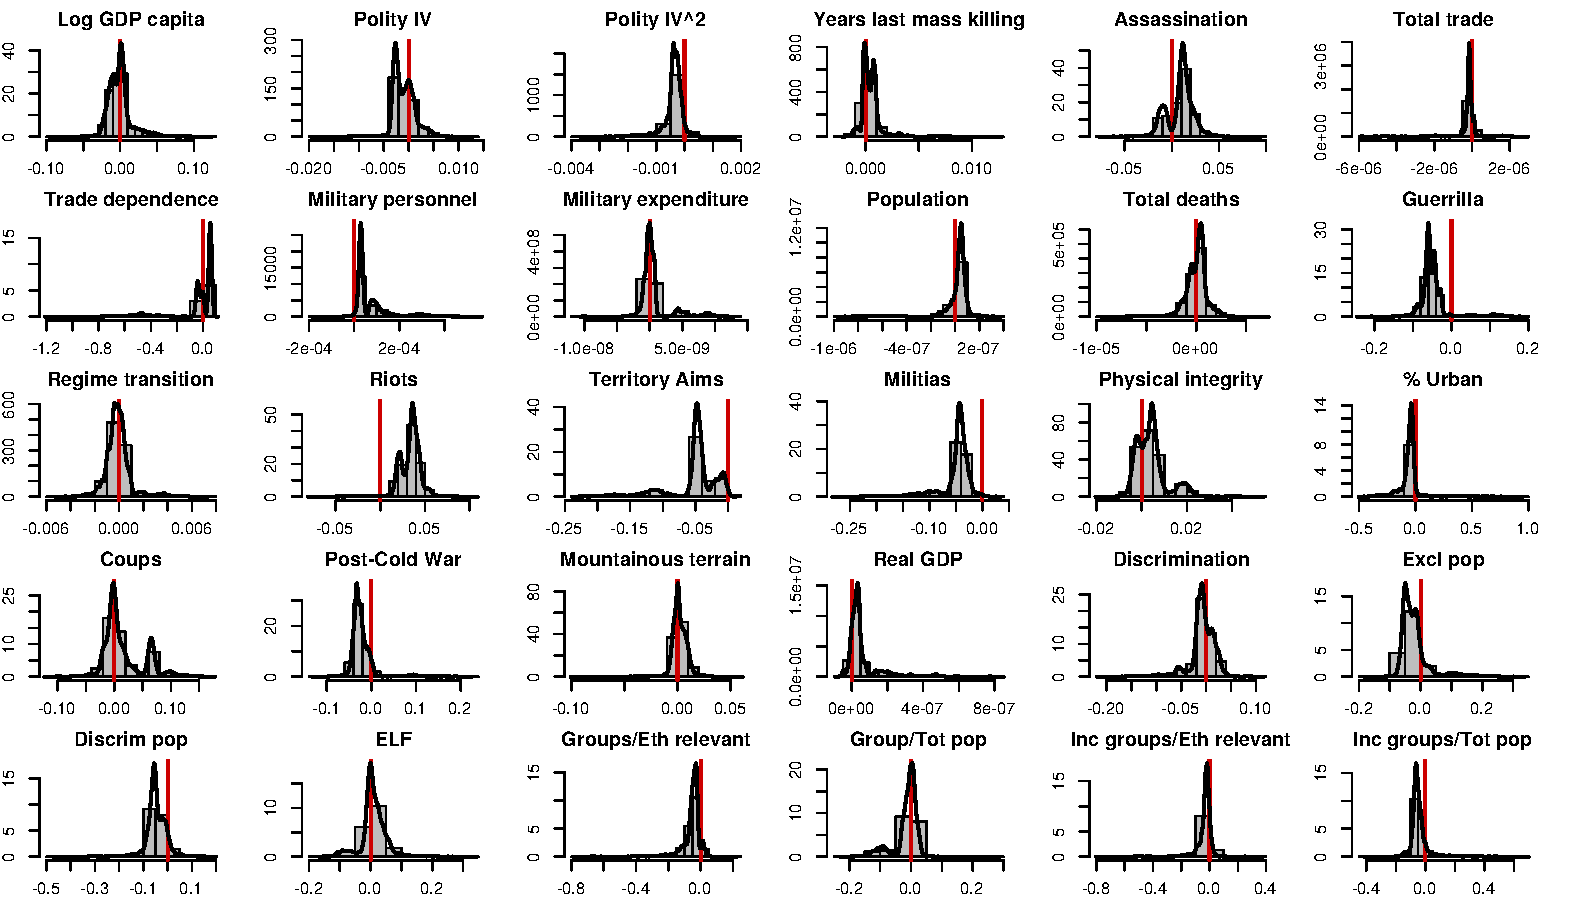
\includegraphics[width=\textwidth]{images/mk-eth.pdf}
    \caption{EBA -- Mass Killings during ethnic civil wars (Cederman et al. Data)}
    \label{fig:mk-eth}
\end{sidewaysfigure}
\clearpage

\subsubsection{Alternative Number of Variables}

The models below are based on 50,000 random draws from the full set of all possible regression models. \citet[819]{salaimartin2004determinants} argue that random sampling produces unbiased estimates of the regression coefficients with low computational time. The models presented in section \ref{sec:results4}, however, include the full set of possible regressions.

The following table shows the results of an EBA with 3 variable combinations per model. The results are very similar to those reported above.

\vspace{1cm}

\begin{table}[H]
\centering
\begin{tabular}{lrrrrr}
\hline
\textbf{Variable} & \textbf{Avg. $\beta$} & \textbf{Avg. SE} & \textbf{$\%$ Sig.} & \textbf{CDF(0)} & \textbf{Models} \\ \hline
\textit{Base variables} &  &  &  &  &  \\
Log GDP per capita & 0.0082 & 0.0043 & 81.439 & 0.9504 & 40677 \\
 &  &  &  &  &  \\
\textit{Additional variables} &  &  &  &  &  \\
Post-Cold War years & -0.0121 & 0.0069 & 77.804 & 0.9609 & 5064 \\
UCDP civil war onset & 0.0523 & 0.0292 & 62.561 & 0.9574 & 3304 \\
Previous riots &0.0134 & 0.0084 & 65.936 & 0.9401 & 5064 \\
UCDP ongoing civil war & 0.0177 & 0.0094 & 72.367 & 0.9372 & 3304 \\
Polity IV squared & -0.0002 & 0.0001 & 66.035 & 0.9268 & 5064 \\ 
Ethnic diversity (ELF) & 0.0162 & 0.0110 & 70.794 & 0.9266 & 5064 \\\hline
\end{tabular}
\caption{EBA -- 3 Variables}
\label{tab:mk-3vars}
\end{table}

\clearpage
\begin{sidewaysfigure}
    \centering
    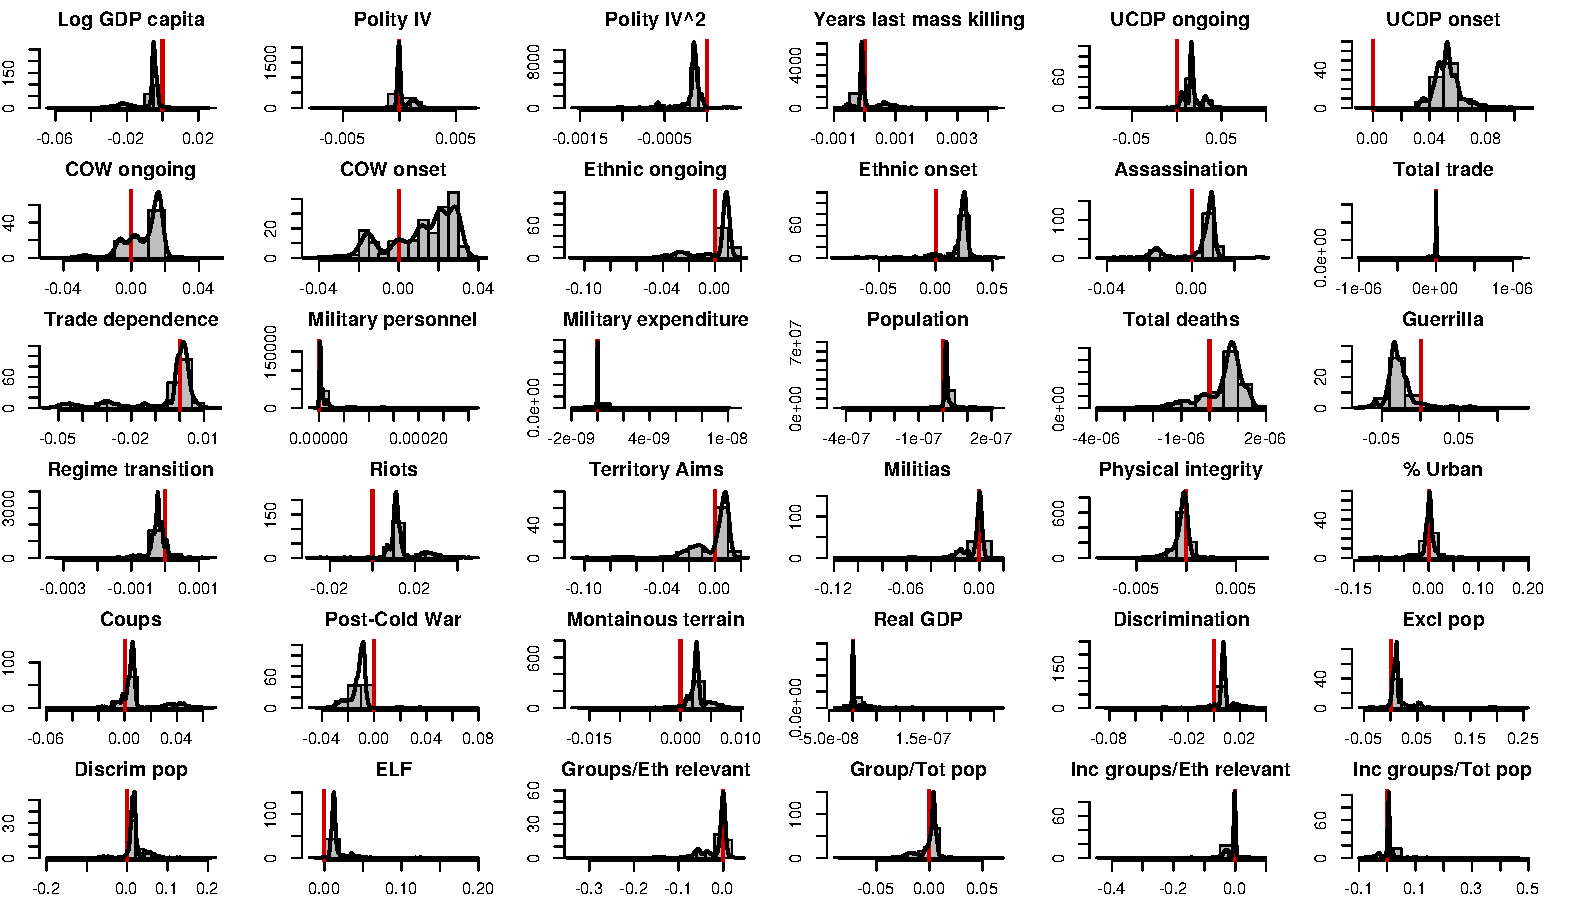
\includegraphics[width=\textwidth]{images/mk-3vars.pdf}
    \caption{EBA -- 3 Variables}
    \label{fig:mk-3vars}
\end{sidewaysfigure}
\clearpage

Table \ref{tab:mk-5vars} presents the results for models with up 5 variables in each regressions. In contrast with the main EBA model, the indicators of UCDP ongoing civil wars, ethnic diversity, and Polity IV square drop out of significance. Their individual CDFs(0) are about 0.88, just marginally below our specified threshold of 0.9.

\vspace{1cm}

\begin{table}[!htpb]
\centering
\begin{tabular}{lrrrrr}
\hline
\textbf{Variable} & \textbf{Avg. $\beta$} & \textbf{Avg. SE} & \textbf{$\%$ Sig.} & \textbf{CDF(0)} & \textbf{Models} \\ \hline
\textit{Base variables} &  &  &  &  &  \\
Log GDP per capita & -0.010 & 0.006 & 70.806 & 0.9161 & 50000 \\
 &  &  &  &  &  \\
\textit{Additional variables} &  &  &  &  &  \\
Post-Cold War years & -0.014 & 0.010 & 68.496 & 0.9336 & 9532 \\
UCDP civil war onset & 0.053 & 0.035 & 44.784 & 0.9308 & 5100 \\
Previous riots & 0.015 & 0.012 & 47.988 & 0.9047 & 9569 \\\hline
\end{tabular}
\caption{EBA -- 5 Variables}
\label{tab:mk-5vars}
\end{table}

\clearpage
\begin{sidewaysfigure}
    \centering
    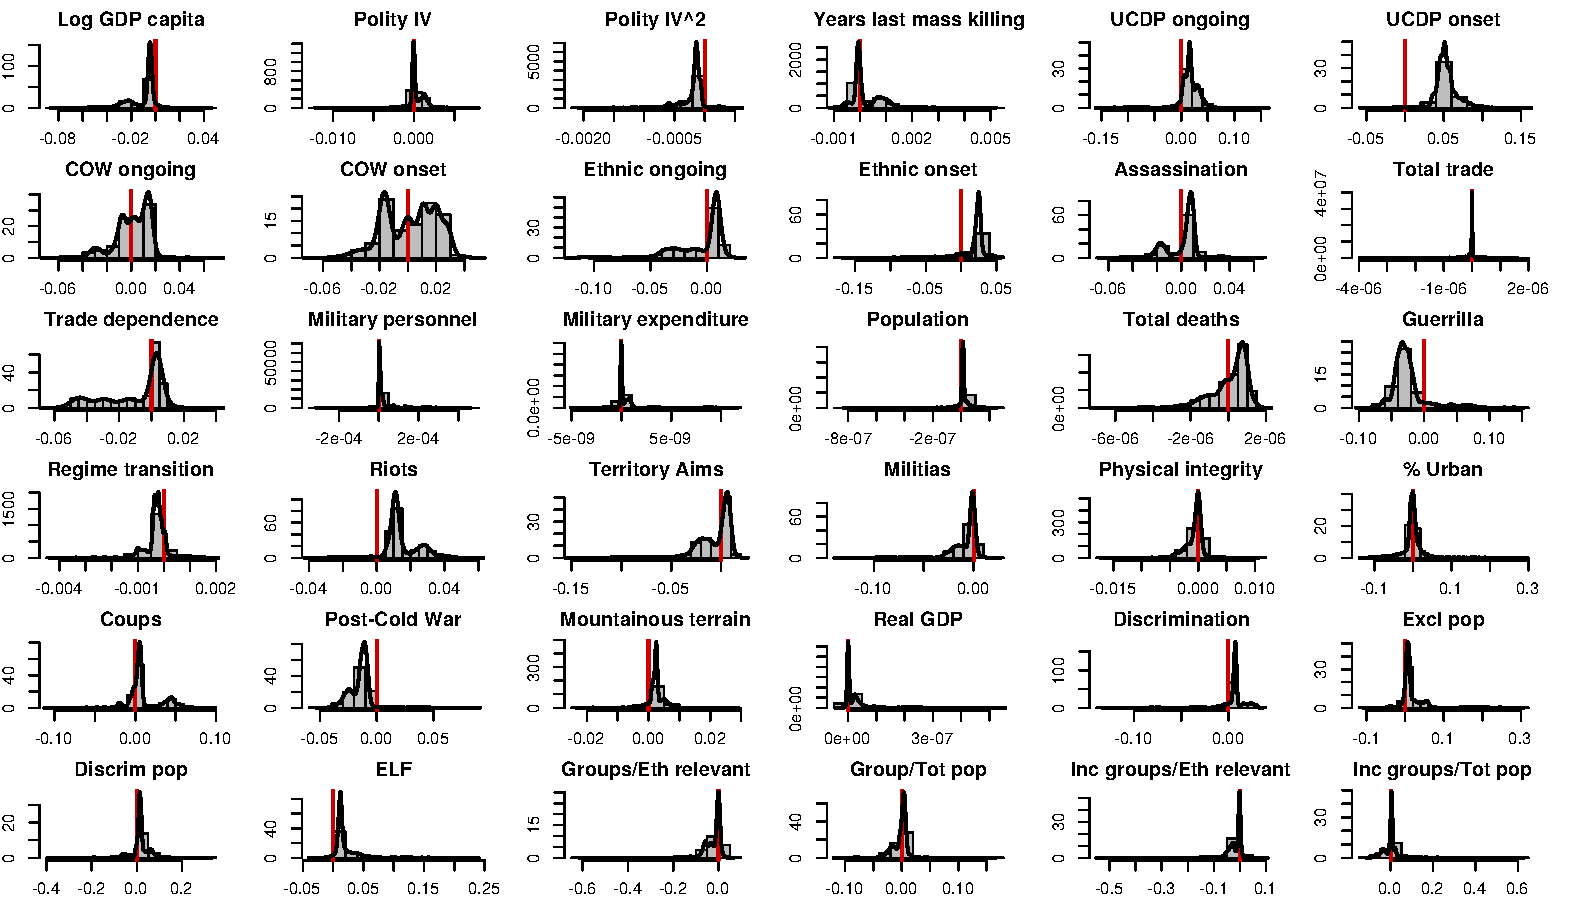
\includegraphics[width=\textwidth]{images/mk-5vars.pdf}
    \caption{EBA -- 5 Variables}
    \label{fig:mk-5vars}
\end{sidewaysfigure}
\clearpage

\subsubsection{Alternative Variance Inflation Factors}

In this subsection, I estimate EBA models with different values of Variance Inflation Factor (VIF), which is a measure of multicollinearity. There is no standard definition about what constitutes an acceptable VIF value, although researchers often use 10 as rule of thumb to indicate strong multicollinearity \citep[674]{o2007caution}. My original model used a slightly more conservative value of 7 as a cutoff. Here, I test the same model with VIF $=$ 10 (less strict), 2.5 (more conservative), and a model without VIF restrictions. The results are essentially identical to those of the main model. In the model with no VIF restriction, however, ethnic fractionalisation fails to meet the threshold by a very small margin. The CDF(0) of that covariate is 0.897, very close to the required value of 0.9. 

\vspace{1cm}

\begin{table}[H]
\centering
\begin{tabular}{lrrrrr}
\hline
\textbf{Variable} & \textbf{Avg. $\beta$} & \textbf{Avg. SE} & \textbf{$\%$ Sig.} & \textbf{CDF(0)} & \textbf{Models} \\ \hline
\textit{Base variables} &  &  &  &  &  \\
Log GDP per capita & -0.0091 & 0.0052 & 76.354 & 0.9343 & 50000 \\
 &  &  &  &  &  \\
\textit{Additional variables} &  &  &  &  &  \\
Post-Cold War years & -0.0134 & 0.0084 & 73.540 & 0.9495 & 7929 \\
UCDP civil war onset & 0.0529 & 0.0322 & 52.141 & 0.9438 & 4553 \\
Previous riots & 0.0140 & 0.0100 & 56.433 & 0.9216 & 7772 \\
UCDP ongoing civil war & 0.0172 & 0.0113 & 66.013 & 0.9113 & 4587 \\
Ethnic diversity (ELF) & 0.0182 & 0.0136 & 56.872 & 0.9056 & 8076 \\
Polity IV squared & -0.0002 & 0.0001 & 60.791 & 0.9021 & 7835 \\ \hline
\end{tabular}
\caption{EBA -- VIF 10}
\label{tab:mk-high-vif}
\end{table}


\clearpage
\begin{sidewaysfigure}
    \centering
    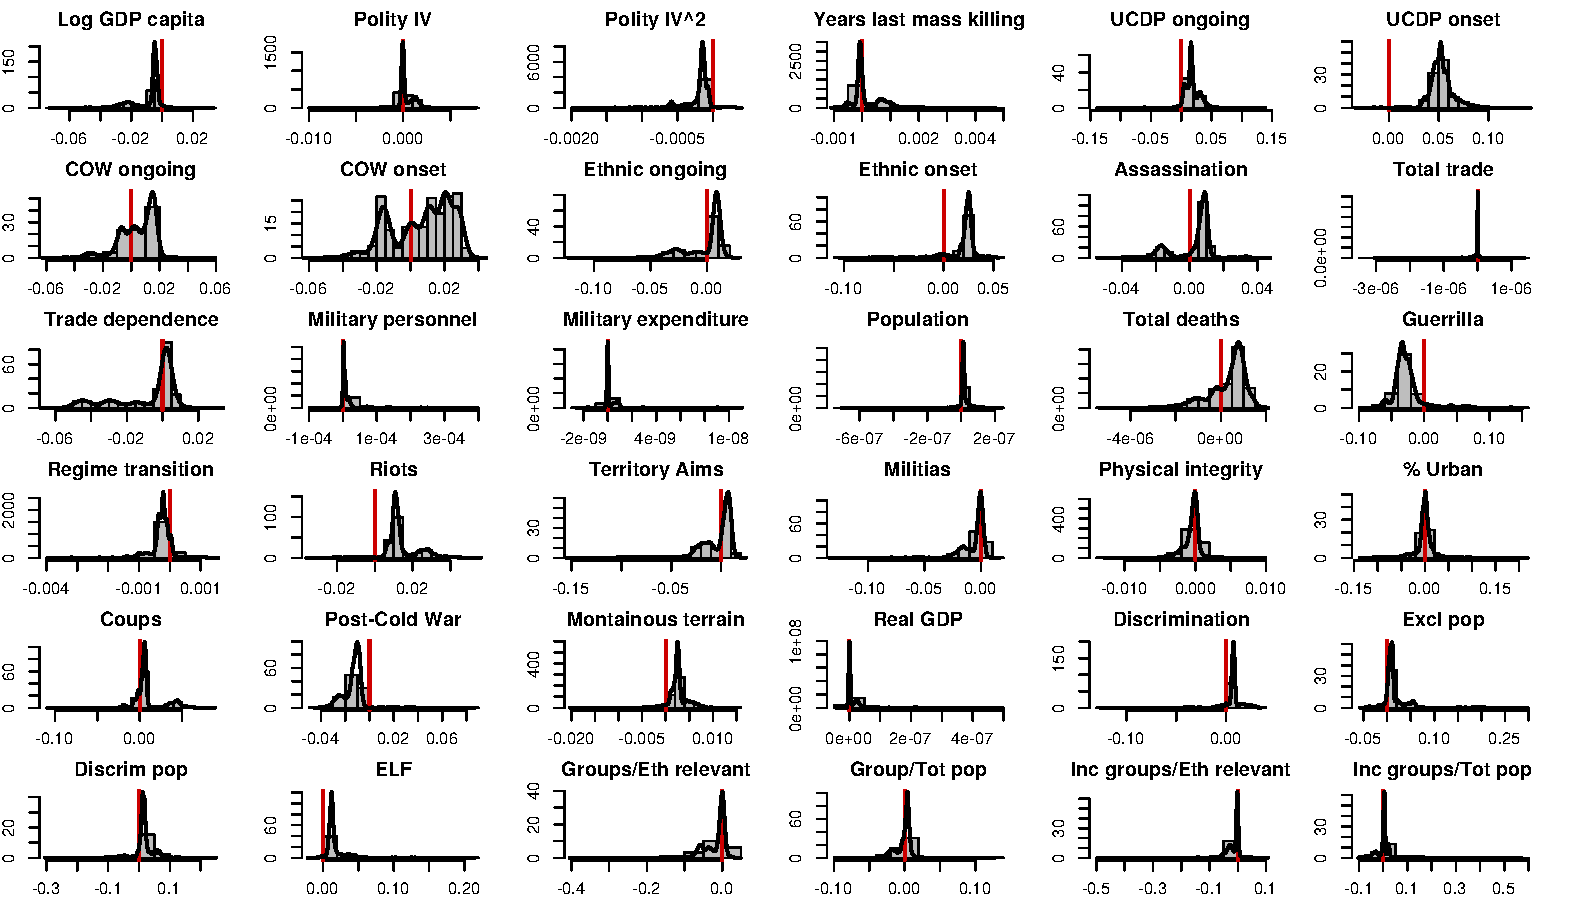
\includegraphics[width=\textwidth]{images/mk-high-vif.pdf}
    \caption{EBA -- VIF 10}
    \label{fig:mk-high-vif}
\end{sidewaysfigure}
\clearpage

\vspace{1cm}

\begin{table}[H]
\centering
\begin{tabular}{lrrrrr}
\hline
\textbf{Variable} & \textbf{Avg. $\beta$} & \textbf{Avg. SE} & \textbf{$\%$ Sig.} & \textbf{CDF(0)} & \textbf{Models} \\ \hline
\textit{Base variables} &  &  &  &  &  \\
Log GDP per capita & -0.0090 & 0.0051 & 76.055 & 0.9343 & 49620 \\
 &  &  &  &  &  \\
\textit{Additional variables} &  &  &  &  &  \\
Post-Cold War years & -0.0132 & 0.0084 & 72.845 & 0.9490 & 7929 \\
UCDP civil war onset & 0.0529 & 0.0322 & 52.378 & 0.9438 & 4553 \\
Previous riots & 0.0141 & 0.0101 & 56.242 & 0.9199 & 7772 \\
UCDP ongoing civil war & 0.0174 & 0.0114 & 65.652 & 0.9103 & 4587 \\
Ethnic diversity (ELF) & 0.0184 & 0.0137 & 56.674 & 0.9054 & 8076 \\
Polity IV squared & -0.0002 & 0.0001 & 61.206 & 0.90267 & 7835 \\ \hline
\end{tabular}
\caption{EBA -- VIF 2.5}
\label{tab:low-vif}
\end{table}

\clearpage
\begin{sidewaysfigure}
    \centering
    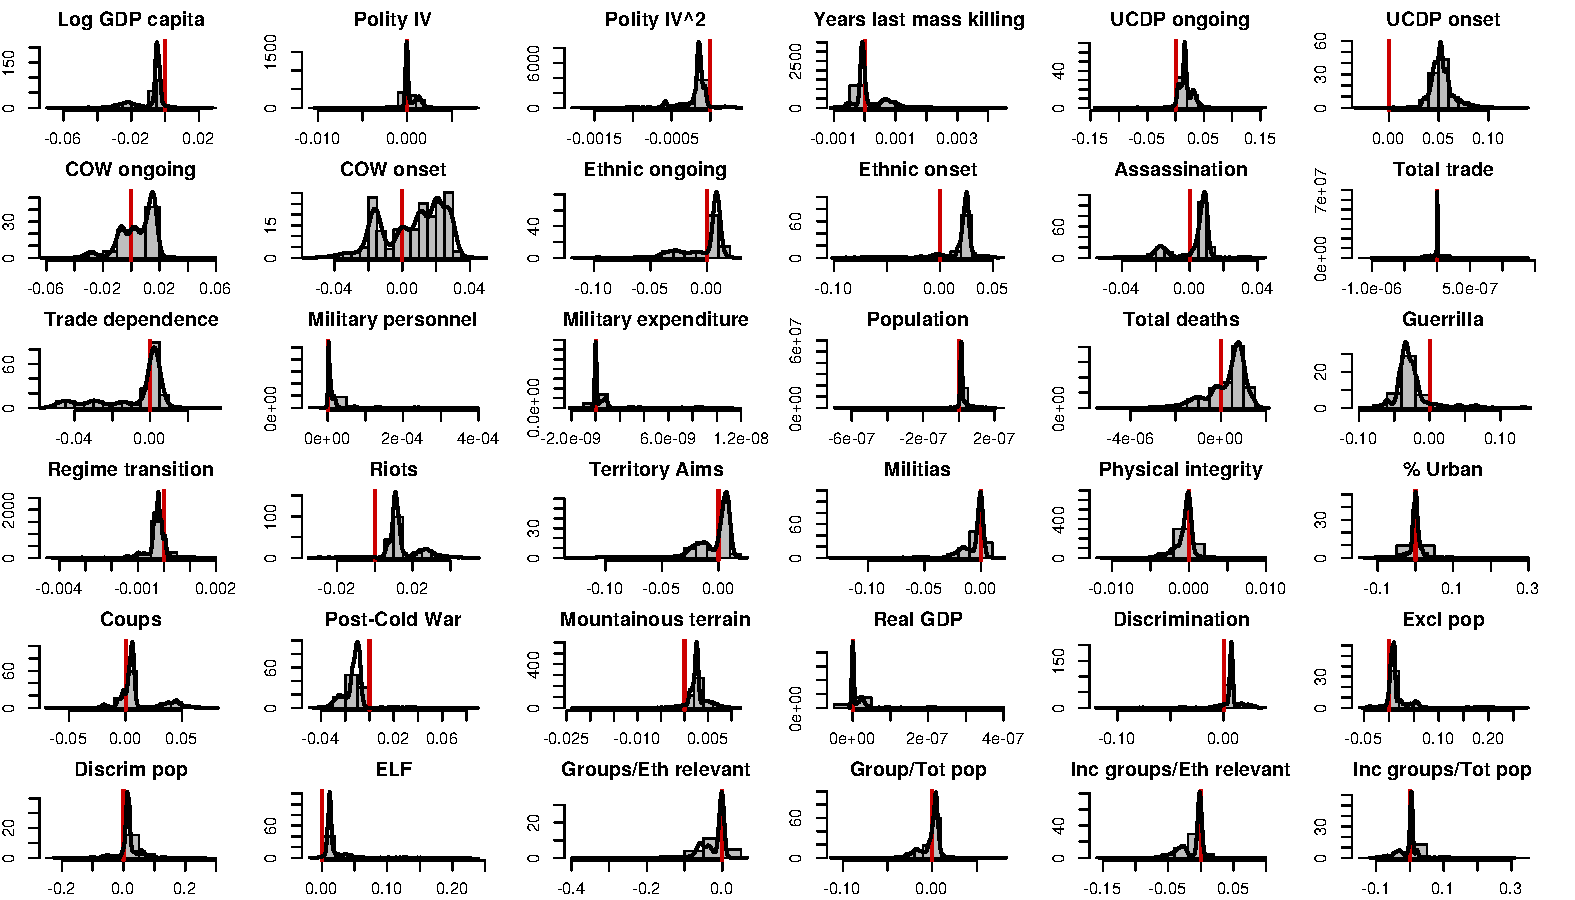
\includegraphics[width=\textwidth]{images/mk-low-vif.pdf}
    \caption{EBA -- VIF 2.5}
    \label{fig:mk-low-vif}
\end{sidewaysfigure}
\clearpage

\begin{table}[H]
\centering
\begin{tabular}{lrrrrr}
\hline
\textbf{Variable} & \textbf{Avg. $\beta$} & \textbf{Avg. SE} & \textbf{$\%$ Sig.} & \textbf{CDF(0)} & \textbf{Models} \\ \hline
\textit{Base variables} &  &  &  &  &  \\
Log GDP per capita & -0.0091 & 0.0052 & 75.940 & 0.9343 & 50000 \\
 &  &  &  &  &  \\
\textit{Additional variables} &  &  &  &  &  \\
Post-Cold War years & -0.0133 & 0.0085 & 72.756 & 0.9469 & 7800 \\
UCDP civil war onset & 0.0531 & 0.0321 & 53.068 & 0.9452 & 4596 \\
Previous riots & 0.0140 & 0.0101 & 56.139 & 0.9200 & 7811 \\
UCDP ongoing civil war & 0.0170 & 0.0116 & 64.487 & 0.9057 & 4497 \\
Ethnic diversity (ELF) & 0.0184 & 0.0137 & 56.814 & 0.9056 & 7808 \\
Polity IV squared & -0.0002 & 0.0001 & 60.825 & 0.9009 & 7903 \\ \hline
\end{tabular}
\caption{EBA -- No VIF Restriction}
\label{tab:mk-no-vif}
\end{table}

\clearpage
\begin{sidewaysfigure}
    \centering
    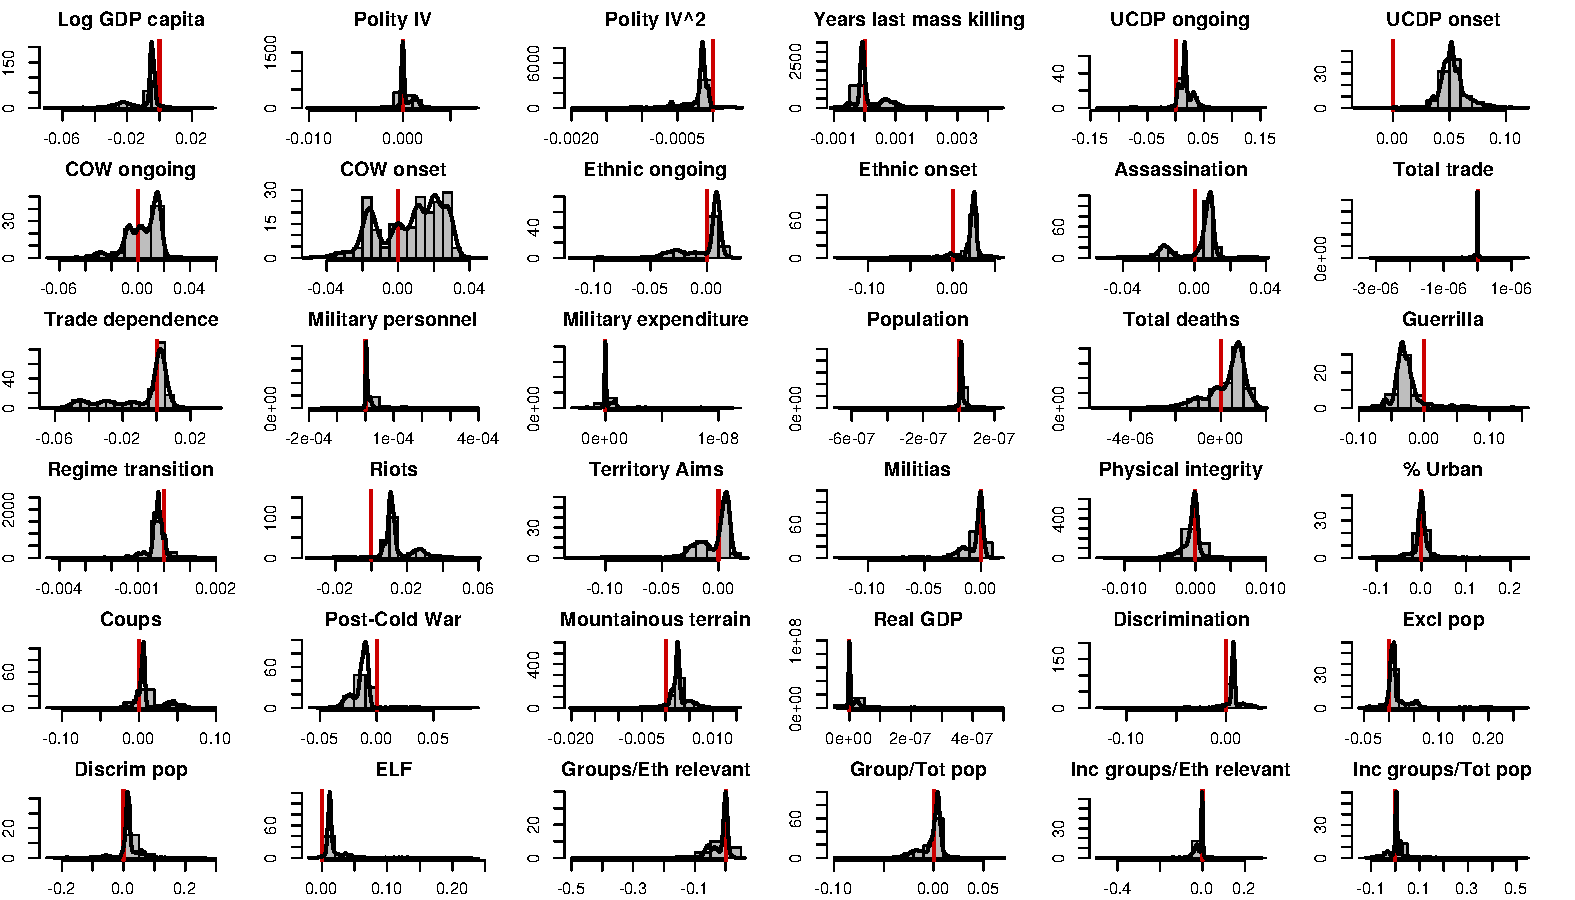
\includegraphics[width=\textwidth]{images/mk-no-vif.pdf}
    \caption{EBA -- No VIF restriction}
    \label{fig:mk-no-vif}
\end{sidewaysfigure}
\clearpage

\subsubsection{Generalised Linear Models}

I reestimate the main EBA model with logit and probit models. Nevertheless, logistic and probit regressions may have issues of complete separation, that is, some covariates may perfectly separate zeros and ones in the outcome variable. In that case, the estimations fail to converge. We address this problem by adding a weak prior to the regression coefficients as suggested by \citet{gelman2008weakly}.\footnote{I thank Mark Bell for sharing \texttt{R} code to estimate penalised-likelihood models.} First, we scaled the non-binary variables to have a mean of 0 and a standard deviation of 0.5, then added a Cauchy distribution with centre 0 and scale 2.5. The probit regressions use a scale of $2.5 \times 1.6$, which is also recommended by the authors \citep{arm2017rpackage}. Ethnic diversity and ongoing civil wars come close to meeting our threshold values (0.88 and 0.84, respectively), and civil war onset (UCDP) has a higher percentage of significant coefficients and a high CDF(0) area than in the linear probability models.

\vspace{1cm}

\begin{table}[H]
\centering
\begin{tabular}{lrrrrr}
\hline
\textbf{Variable} & \textbf{Avg. $\beta$} & \textbf{Avg. SE} & \textbf{$\%$ Sig.} & \textbf{CDF(0)} & \textbf{Models} \\ \hline
\textit{Base variables} &  &  &  &  &  \\
Log GDP per capita & 0.434 & 0.223 & 75.570 & 0.9267 & 50000 \\
 &  &  &  &  &  \\
\textit{Additional variables} &  &  &  &  &  \\
UCDP civil war onset & 1.308 & 0.530 & 87.261 & 0.9742 & 4506 \\
Post-Cold War years & -0.911 & 0.428 & 70.456 & 0.9448 & 7890 \\
Previous riots & 0.744 & 0.38 & 66.778 & 0.9383 & 7805 \\
Polity IV squared & -0.015 & 0.008 & 68.038 & 0.9285 & 7975 \\ \hline
\end{tabular}
\caption{EBA -- Logistic Regression}
\label{tab:mk-logit}
\end{table}

\clearpage
\begin{sidewaysfigure}
    \centering
    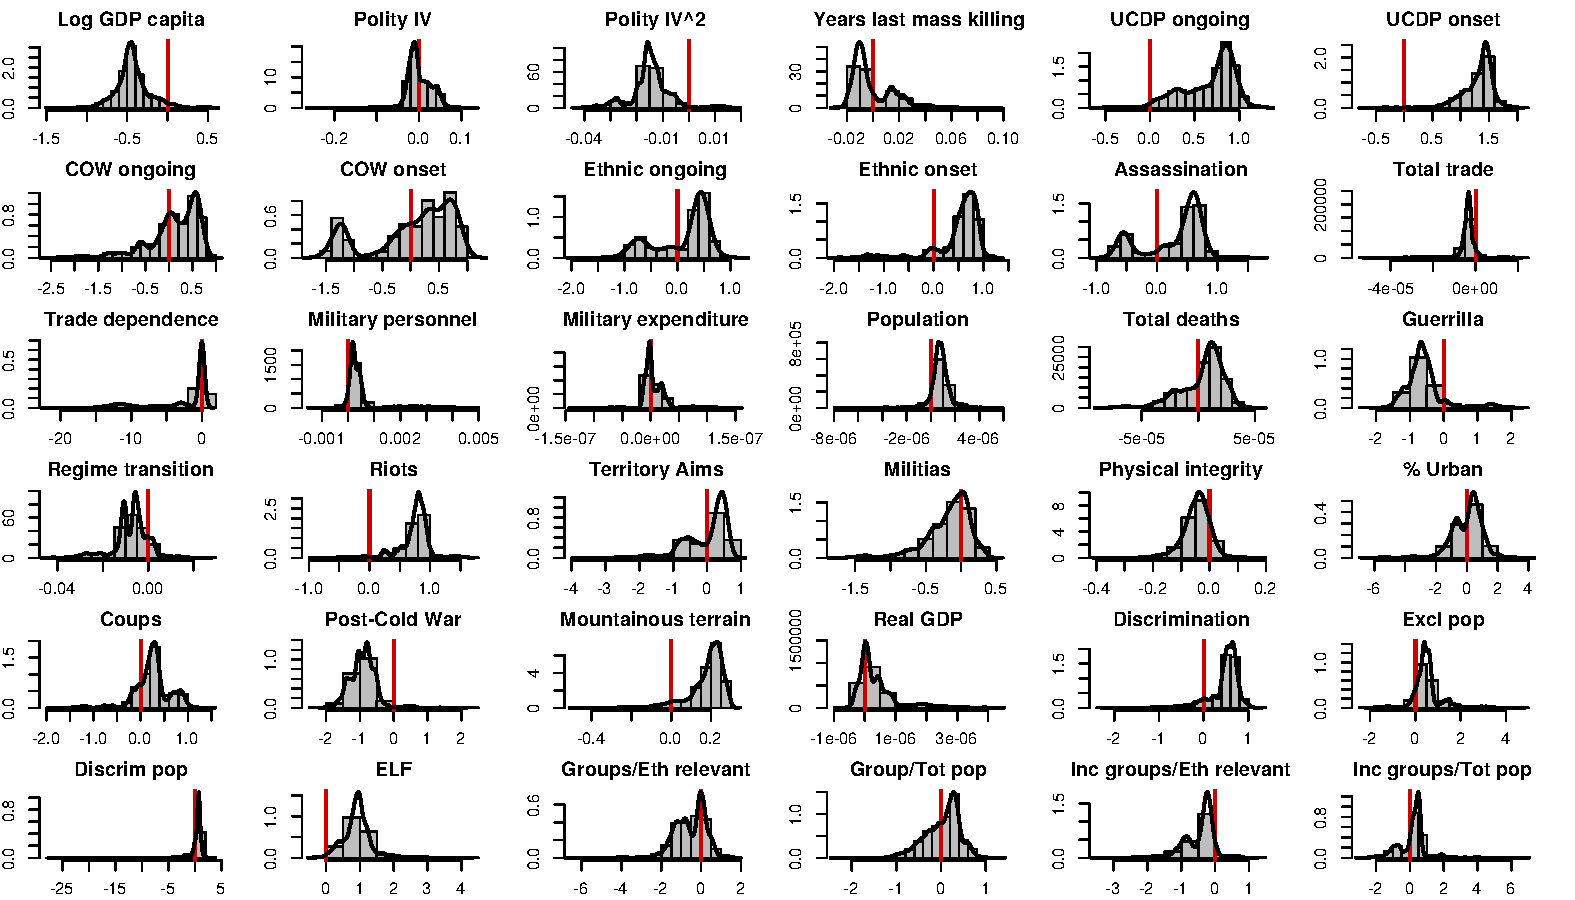
\includegraphics[width=\textwidth]{images/mk-logit.pdf}
    \caption{EBA -- Logistic Regression}
    \label{fig:mk-logit}
\end{sidewaysfigure}
\clearpage

\begin{table}[H]
\centering
\begin{tabular}{lrrrrr}
\hline
\textbf{Variable} & \textbf{Avg. $\beta$} & \textbf{Avg. SE} & \textbf{$\%$ Sig.} & \textbf{CDF(0)} & \textbf{Models} \\ \hline
\textit{Base variables} &  &  &  &  &  \\
Log GDP per capita & -0.1924 & 0.1031 & 76.118 & 0.9258 & 50000 \\
 &  &  &  &  &  \\
\textit{Additional variables} &  &  &  &  &  \\
UCDP civil war onset & 0.6422 & 0.2582 & 89.225 & 0.9772 & 4501 \\
Previous riots & 0.3367 & 0.1743 & 71.813 & 0.9436 & 7851 \\
Post-Cold War years & -0.3709 & 0.1830 & 71.465 & 0.9404 & 7836 \\
Polity IV squared & -0.0061 & 0.0032 & 70.155 & 0.9315 & 7931 \\ \hline
\end{tabular}
\caption{EBA -- Probit Regression}
\label{tab:eba1}
\end{table}

\clearpage
\begin{sidewaysfigure}
    \centering
    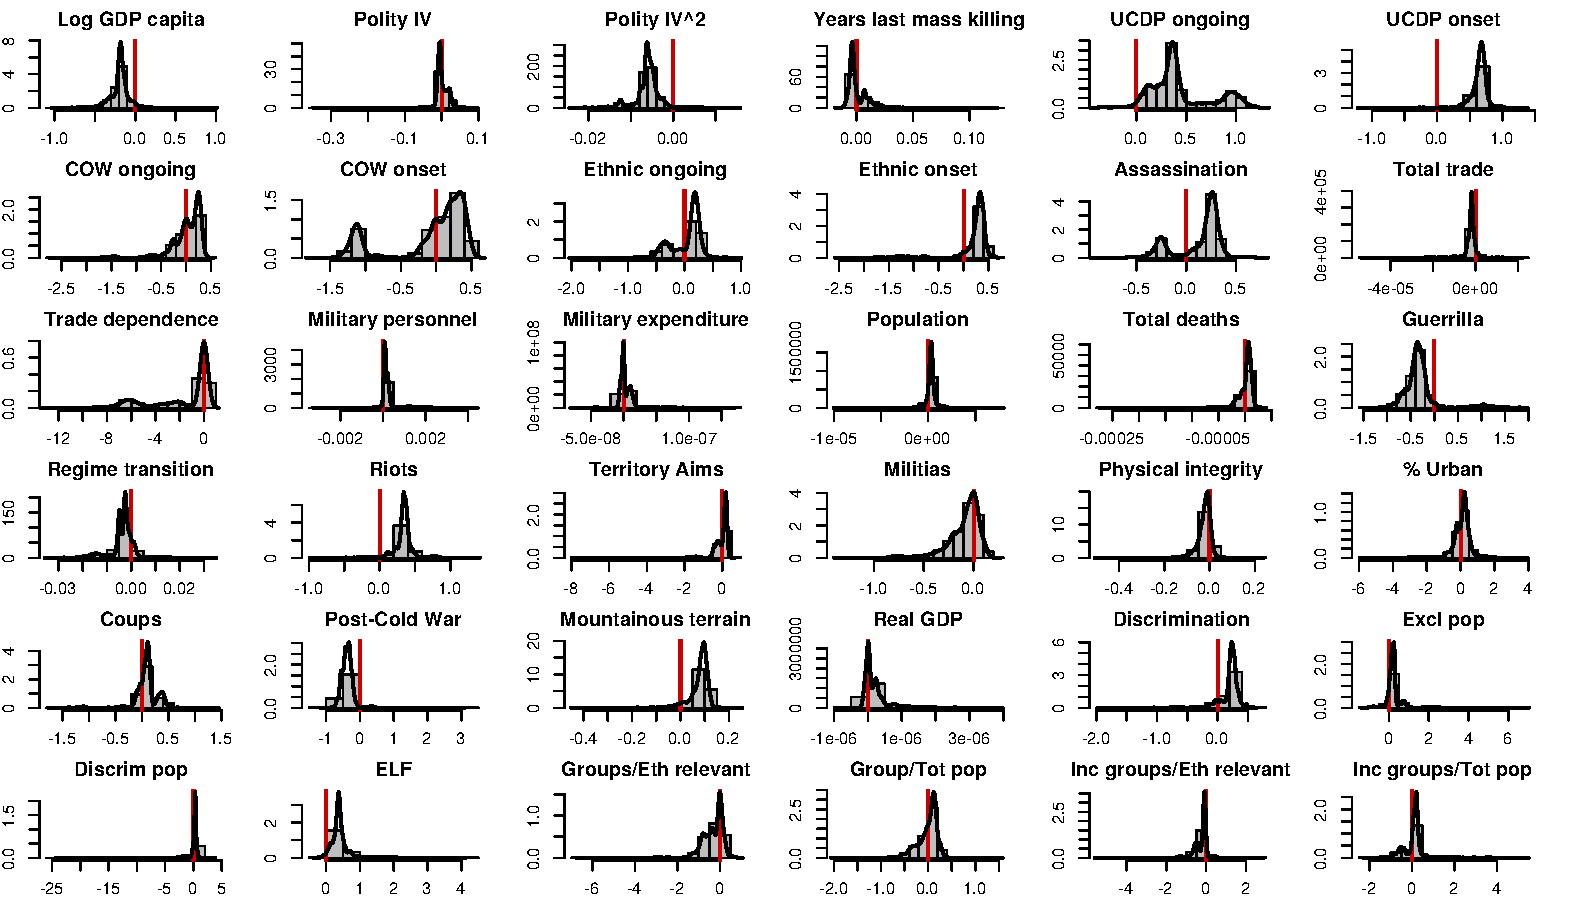
\includegraphics[width=\textwidth]{images/mk-probit.pdf}
    \caption{EBA -- Probit Regression}
    \label{fig:mk-probit}
\end{sidewaysfigure}
\clearpage

\subsubsection{Mass Killings in and after the Cold War}%
\label{sub:mass_killings_in_and_after_the_cold_war}

I also test the heterogeneity of the findings by running one model including only the Cold War years (1945--1991) and another with the post-Cold War period (1991--2013). The results vary in both periods, and there is no overlap between significant variables.

\vspace{.5cm}

\begin{table}[H]
\centering
\begin{tabular}{lrrrrr}
\hline
\textbf{Variable} & \textbf{Avg. $\beta$} & \textbf{Avg. SE} & \textbf{$\%$ Sig.} & \textbf{CDF(0)} & \textbf{Models} \\ \hline
\textit{Cold War Period} &  &  &  &  &  \\
Log GDP per capita & -0.018 & 0.009 & 83.204 & 0.9678 & 50000 \\
Previous riots & 0.022 & 0.014 & 62.457 & 0.9031 & 8278 \\
 &  &  &  &  &  \\
\textit{Post-Cold War Period} &  &  &  &  &  \\
Ethnic war onset & -0.024 & 0.011 & 89.608 & 0.9823 & 4850 \\
Coup d'état & -0.022 & 0.011 & 89.200 & 0.9822 & 8602 \\ 
Territory aims & -0.027 & 0.014 & 81.083 & 0.9653 & 8775 \\ 
Displaced Population & -0.048 & 0.027 & 58.689 & 0.9392 & 8695 \\ \hline
\end{tabular}
\caption{EBA -- Mass Killings in and after the Cold War Period (Robust Variables Only)}
\label{tab:coldwar2}
\end{table}

\clearpage
\begin{sidewaysfigure}
    \centering
    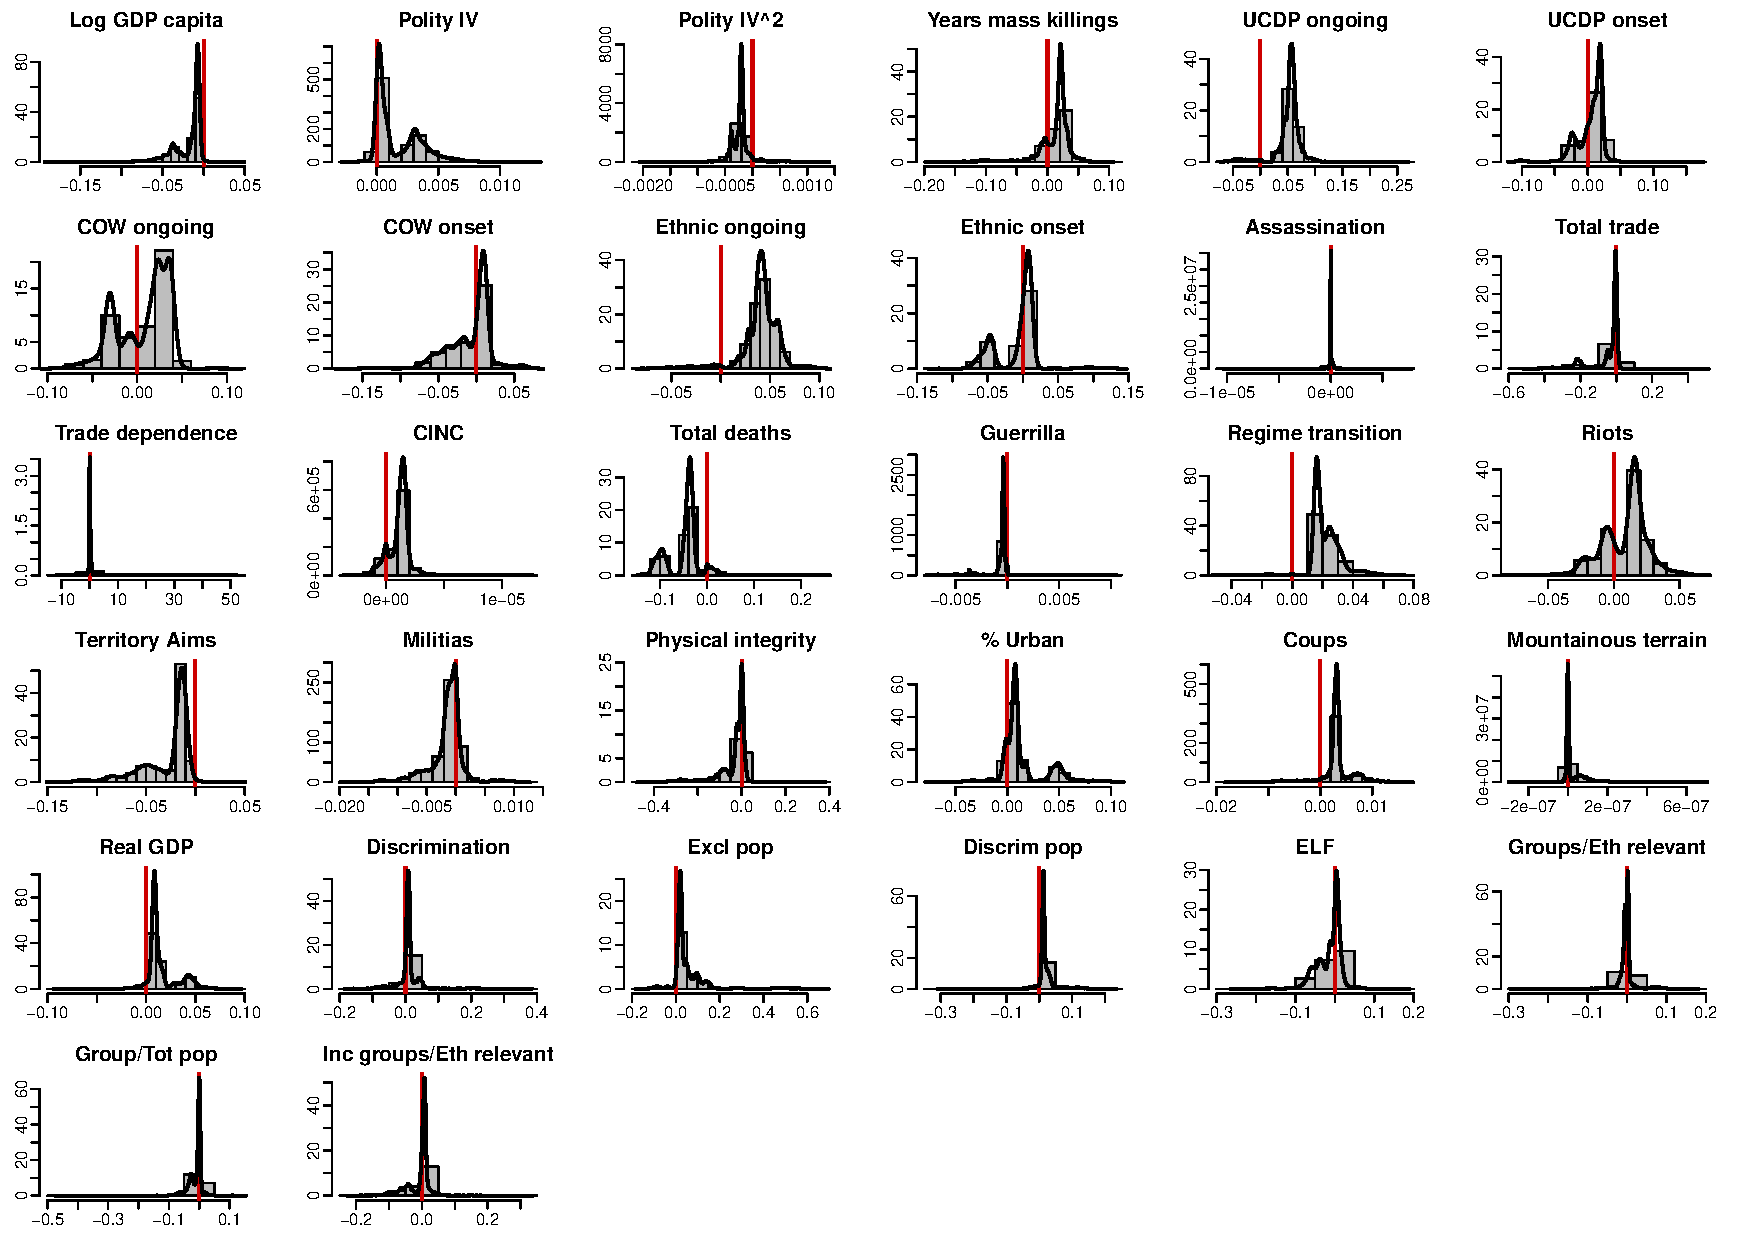
\includegraphics[width=.9\textwidth]{images/mk-coldwar.pdf}
    \caption{EBA -- Cold War Period}
    \label{fig:mk-coldwar}
\end{sidewaysfigure}
\clearpage

\clearpage
\begin{sidewaysfigure}
    \centering
    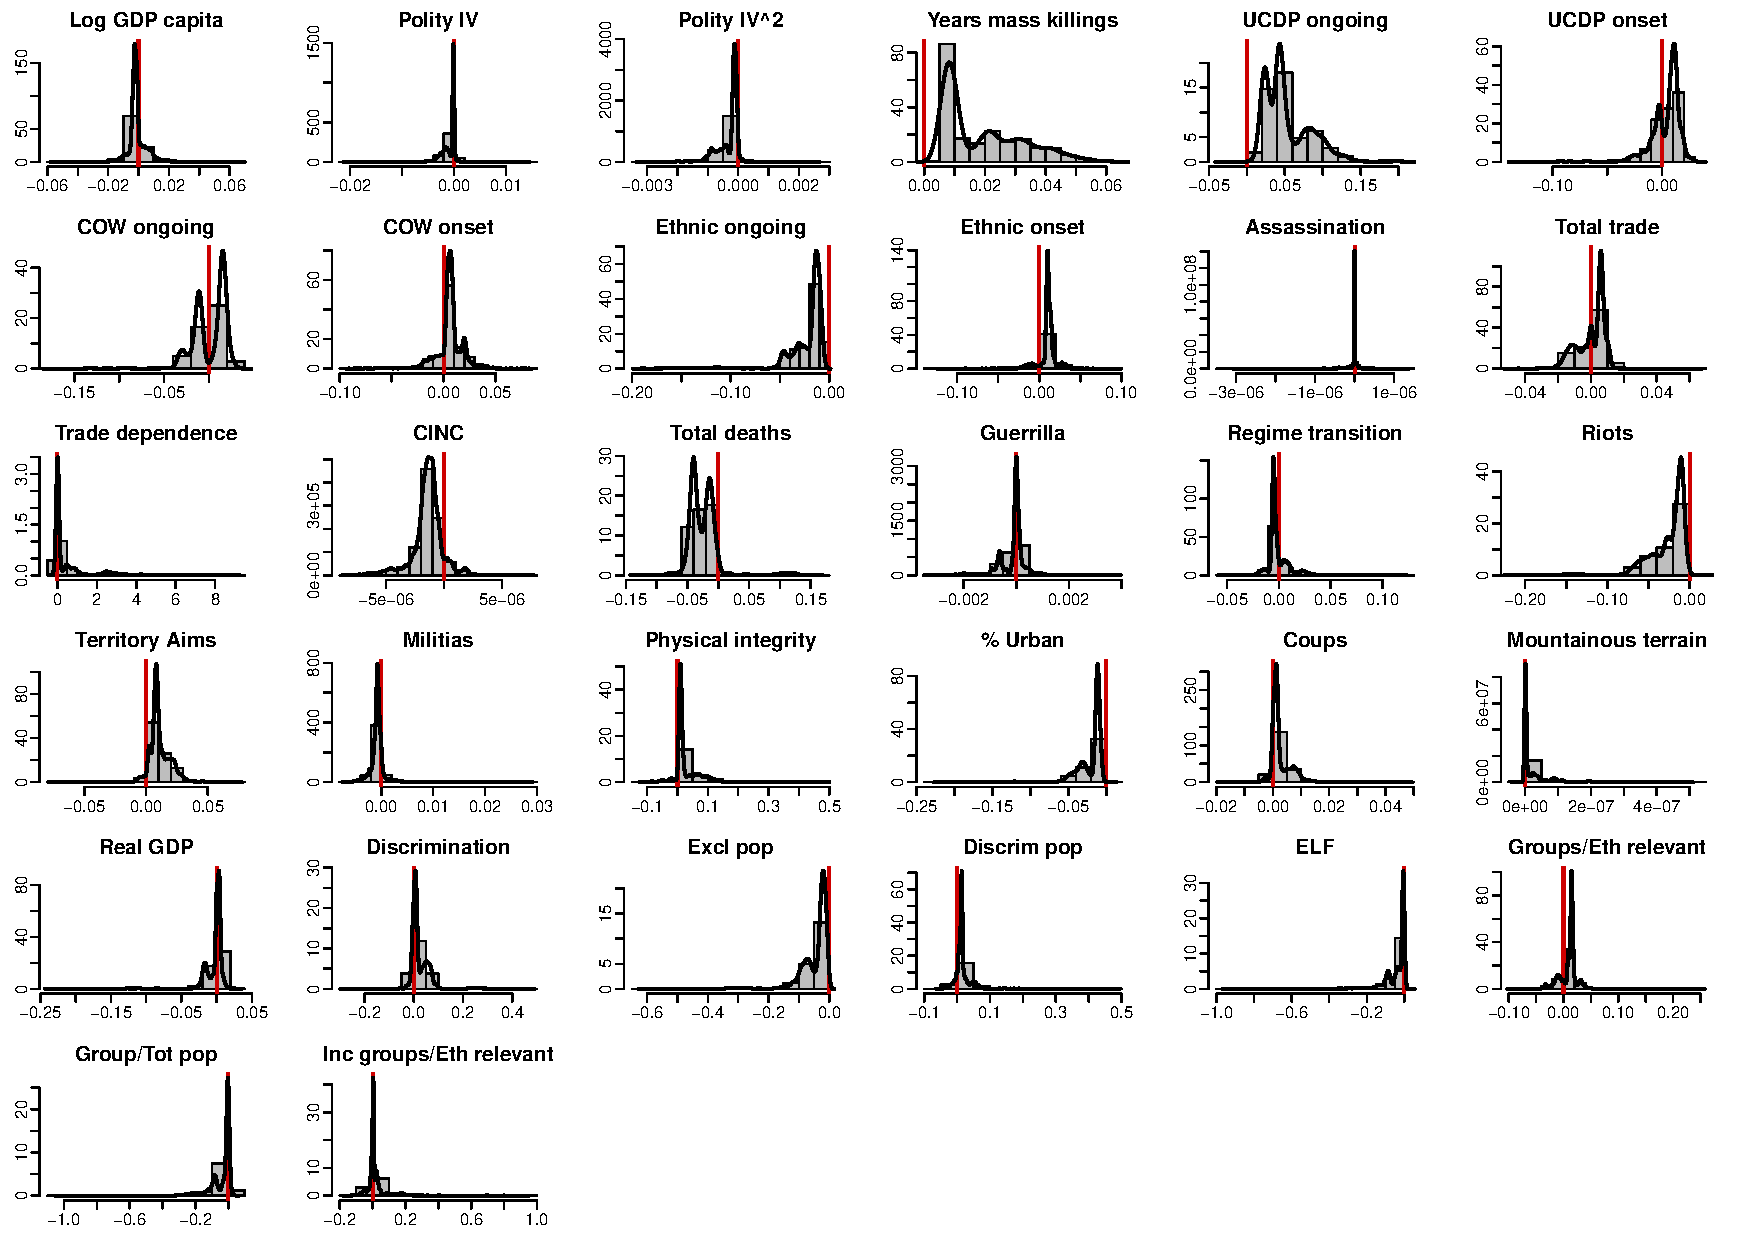
\includegraphics[width=.9\textwidth]{images/mk-postcoldwar.pdf}
    \caption{EBA -- Post-Cold War Period}
    \label{fig:mk-postcoldwar}
\end{sidewaysfigure}
\clearpage

\subsubsection{Mass Killings during Peacetime}

I have also tested whether the main EBA findings differ if the sample is restricted to peace years. That is, all observations denoted as 1 in the three conflict indicators mentioned above (UCDP, COW, Cederman et al.) were removed from the dataset. The results are similar to the main model, yet ``wars fought over territory'' was removed from the EBA due to multicollinearity issues. Moreover, two other variables (total battle deaths and presence of guerrillas) have very small sample sizes and their estimates were should not be interpreted as reliable. The significant variables are presented below.

\vspace{1cm}

\begin{table}[H]
\centering
\begin{tabular}{lrrrrr}
\hline
\textbf{Variable} & \textbf{Avg. $\beta$} & \textbf{Avg. SE} & \textbf{$\%$ Sig.} & \textbf{CDF(0)} & \textbf{Models} \\ \hline
\textit{Base variables} &  &  &  &  &  \\
Log GDP per capita & -0.004 & 0.002 & 86.608 & 0.9748 & 26620 \\
 &  &  &  &  &  \\
\textit{Additional variables} &  &  &  &  &  \\
Post Cold War & -0.011 & 0.003 & 100 & 0.9984 & 5459\\
Polity IV squared & -1.63e-04 & 6.27e-05 & 98.309 & 0.9914 & 5441 \\
Discriminated pop & 0.009 & 0.005 & 92.516 & 0.9750 & 5438 \\
Mountainous terrain & 0.002 & 0.001 & 74.171 & 0.9718 & 5428\\
Population & -9.89e-09 & 6.20e-09 & 61.776 & 0.9280 & 5418 \\
Previous riots  & 0.008 & 0.006 & 28.315 & 0.9119 & 5400\\ \hline
\end{tabular}
\caption{EBA -- VIF 10}
\label{tab:mk-high-vif}
\end{table}

\clearpage
\begin{sidewaysfigure}
    \centering
    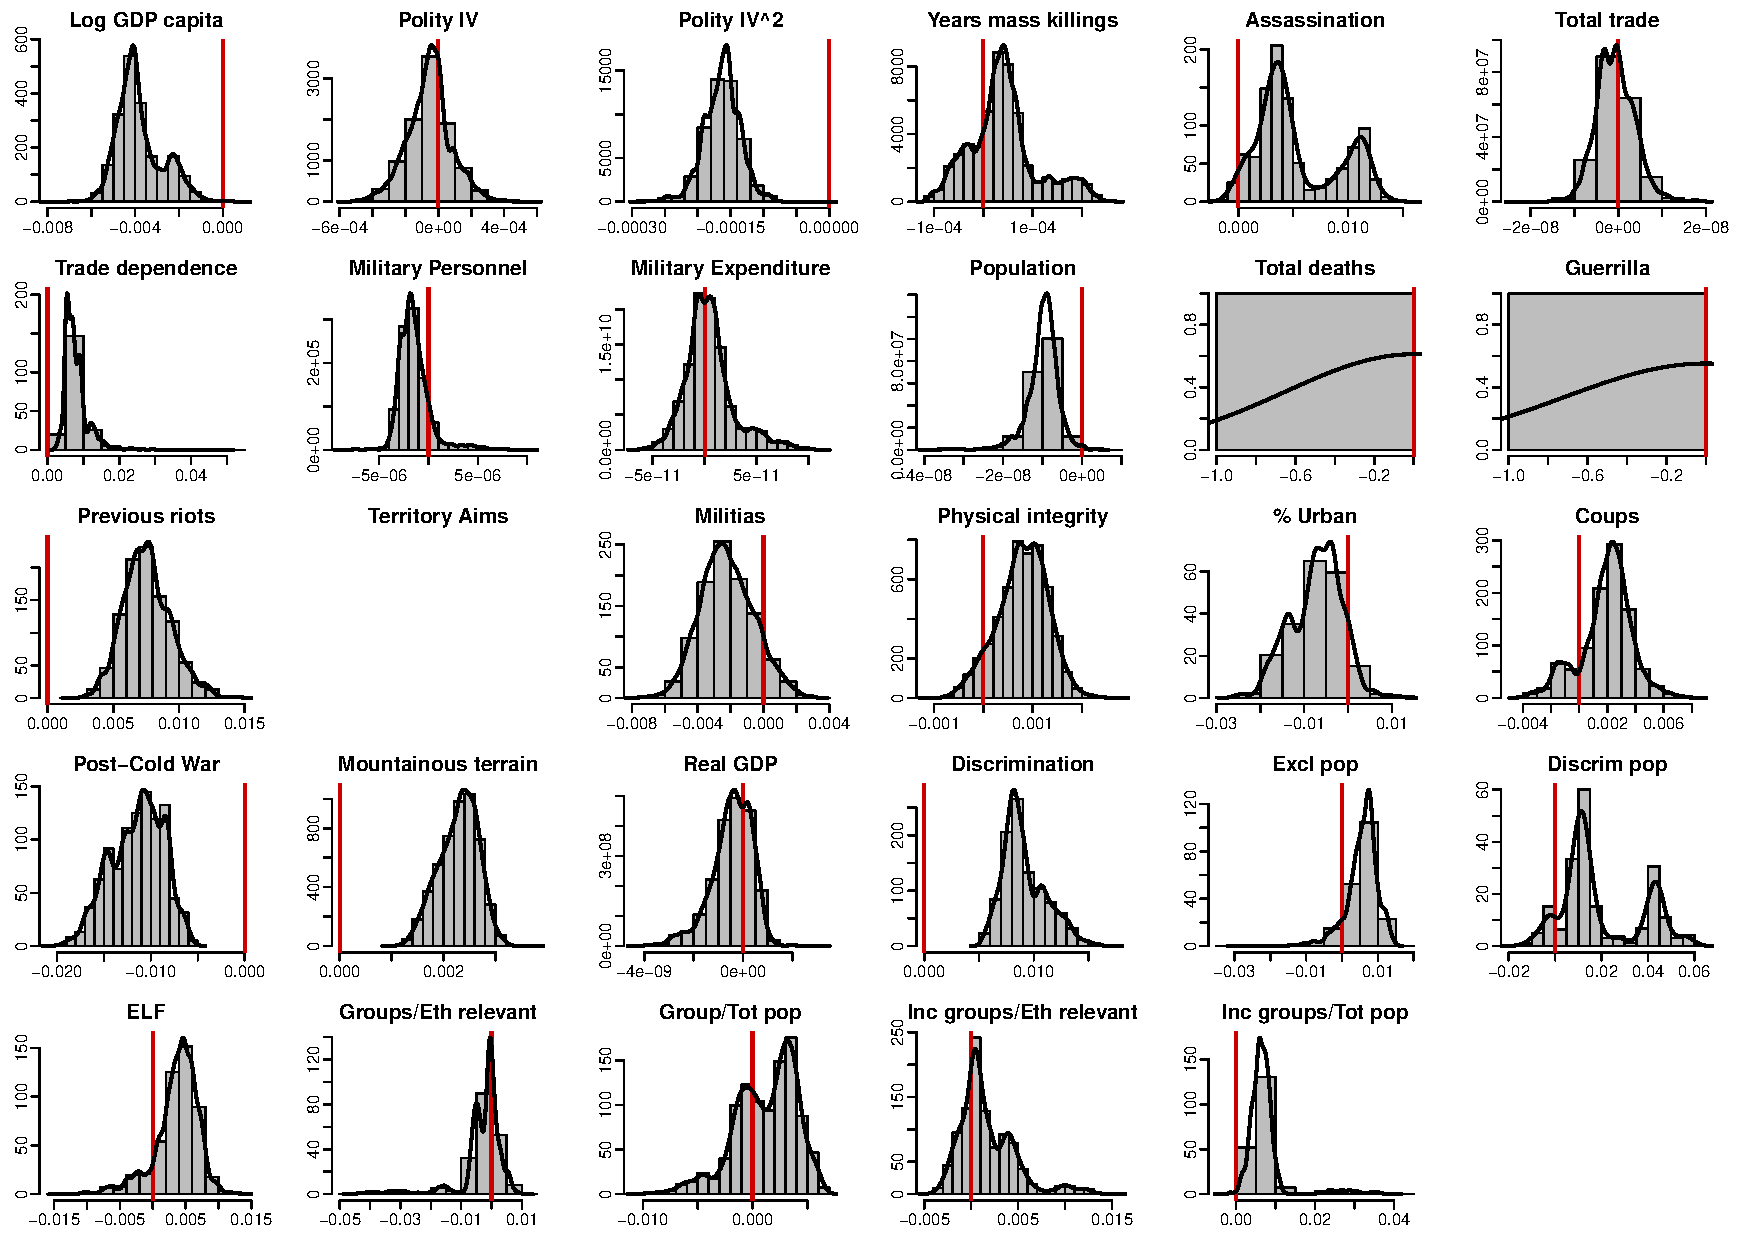
\includegraphics[width=\textwidth]{images/mk-nowar.pdf}
    \caption{EBA -- Peace Years}
    \label{fig:mk-postcoldwar}
\end{sidewaysfigure}
\clearpage

\subsection{Harff's Genocides and Politicides Data}
\label{sec:harff}

\subsubsection{Main Model}

In this section, we evaluate the models presented above with a measure of genocide and politicide by \citet{harff2003no}. The results show important contrasts with the previous analyses. First, no variable appear as significant in the main extreme bounds analysis. That is, none of the 36 predictors reached the threshold of CDF(0) $> 0.9$. Thus, we do not present a table with the results. The variable that came closest to significance was a dummy indicator of coups d'état, which has a CDF(0) of 0.897 and, as expected, is positively correlated with the onset of genocides. The distribution of the covariates' coefficients are available in figure \ref{fig:uamk}.

\newpage 

\clearpage
\begin{sidewaysfigure}
    \centering
    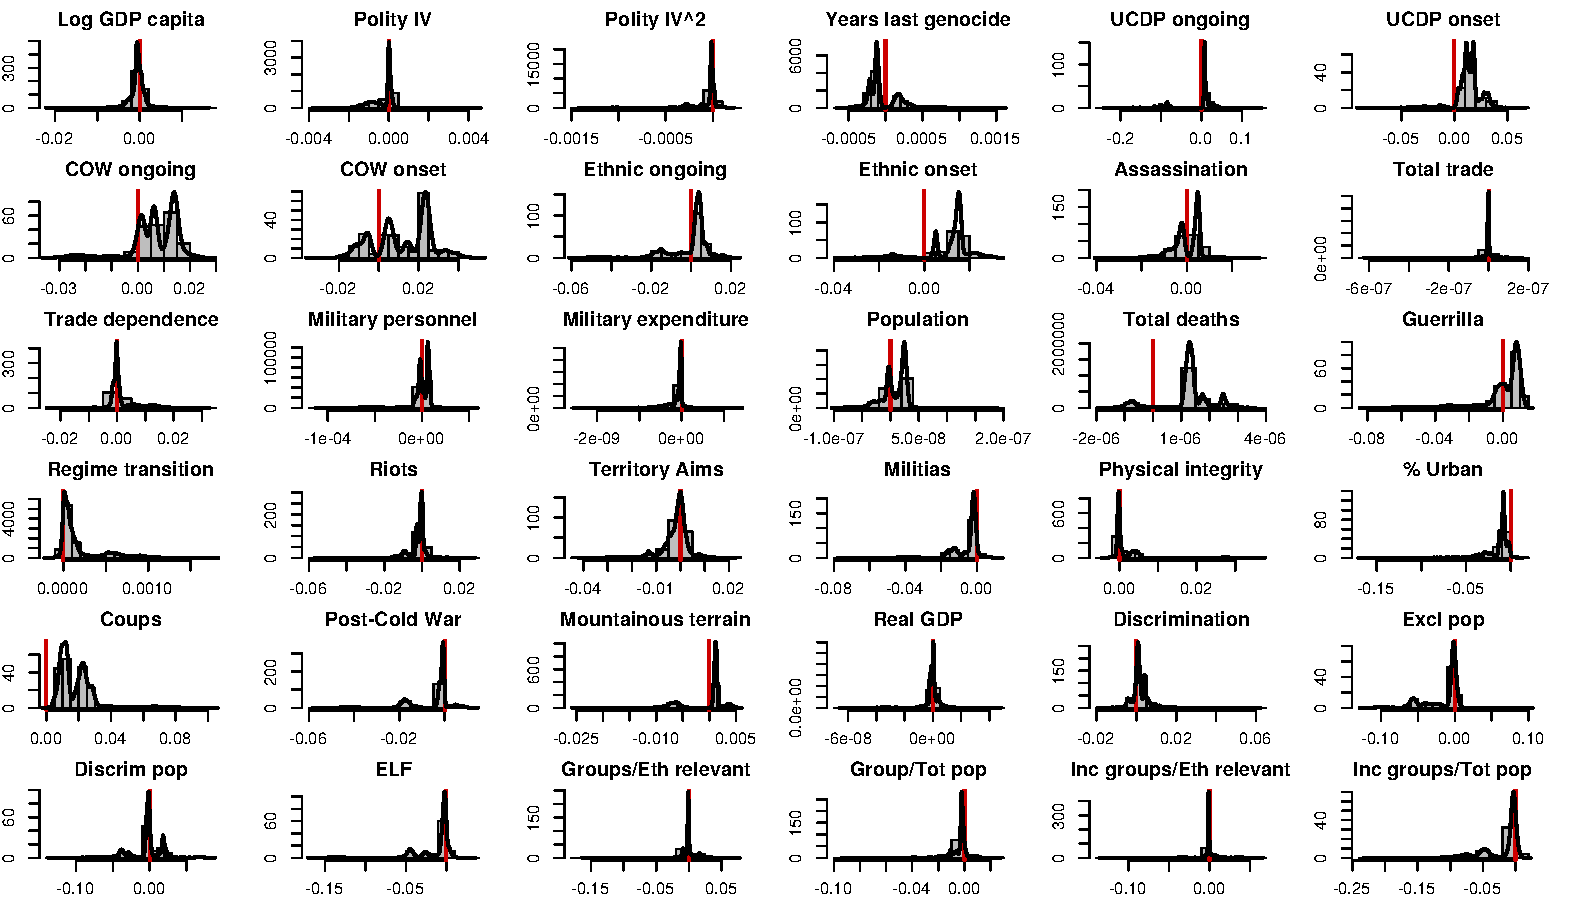
\includegraphics[width=\textwidth]{images/uamk.pdf}
    \caption{EBA -- Genocides and Politicides}
    \label{fig:uamk}
\end{sidewaysfigure}
\clearpage

\subsubsection{Genocides and Politicides during Civil Wars}

Next, we evaluate what covariates are robust when considering only genocides and politicide that occur during civil conflicts. Post-Cold War years again appear as a significant variable and with a negative sign; excluded population also has a negative impact on the outcome variable in two analyses.

\vspace{1cm}

\begin{table}[H]
\centering
\begin{tabular}{lrrrrr}
\hline
\textbf{Variable} & \textbf{Avg. $\beta$} & \textbf{Avg. SE} & \textbf{$\%$ Sig.} & \textbf{CDF(0)} & \textbf{Models} \\ \hline
\textit{UCDP data} &  &  &  &  &  \\
Excluded population & -0.037 & 0.022 & 64.524 & 0.9176 & 8758 \\
 &  &  &  &  &  \\
\textit{COW data} &  &  &  &  &  \\
Excluded population & -0.057 & 0.031 & 65.703 & 0.9570 & 8820 \\
Discriminated population & -0.050 & 0.029 & 53.850 & 0.9367 & 8767 \\
Post-Cold War years & -0.019 & 0.013 & 42.531 & 0.9203 & 8904 \\
 &  &  &  &  &  \\
\textit{Cederman et al. data} &  &  &  &  &  \\
Assassination dummy & -0.009 & 0.006 & 47.723 & 0.9232 & 8828 \\ \hline
\end{tabular}
\caption{EBA -- Genocides/Politicides}
\label{tab:uamk1}
\end{table}

\clearpage
\begin{sidewaysfigure}
    \centering
    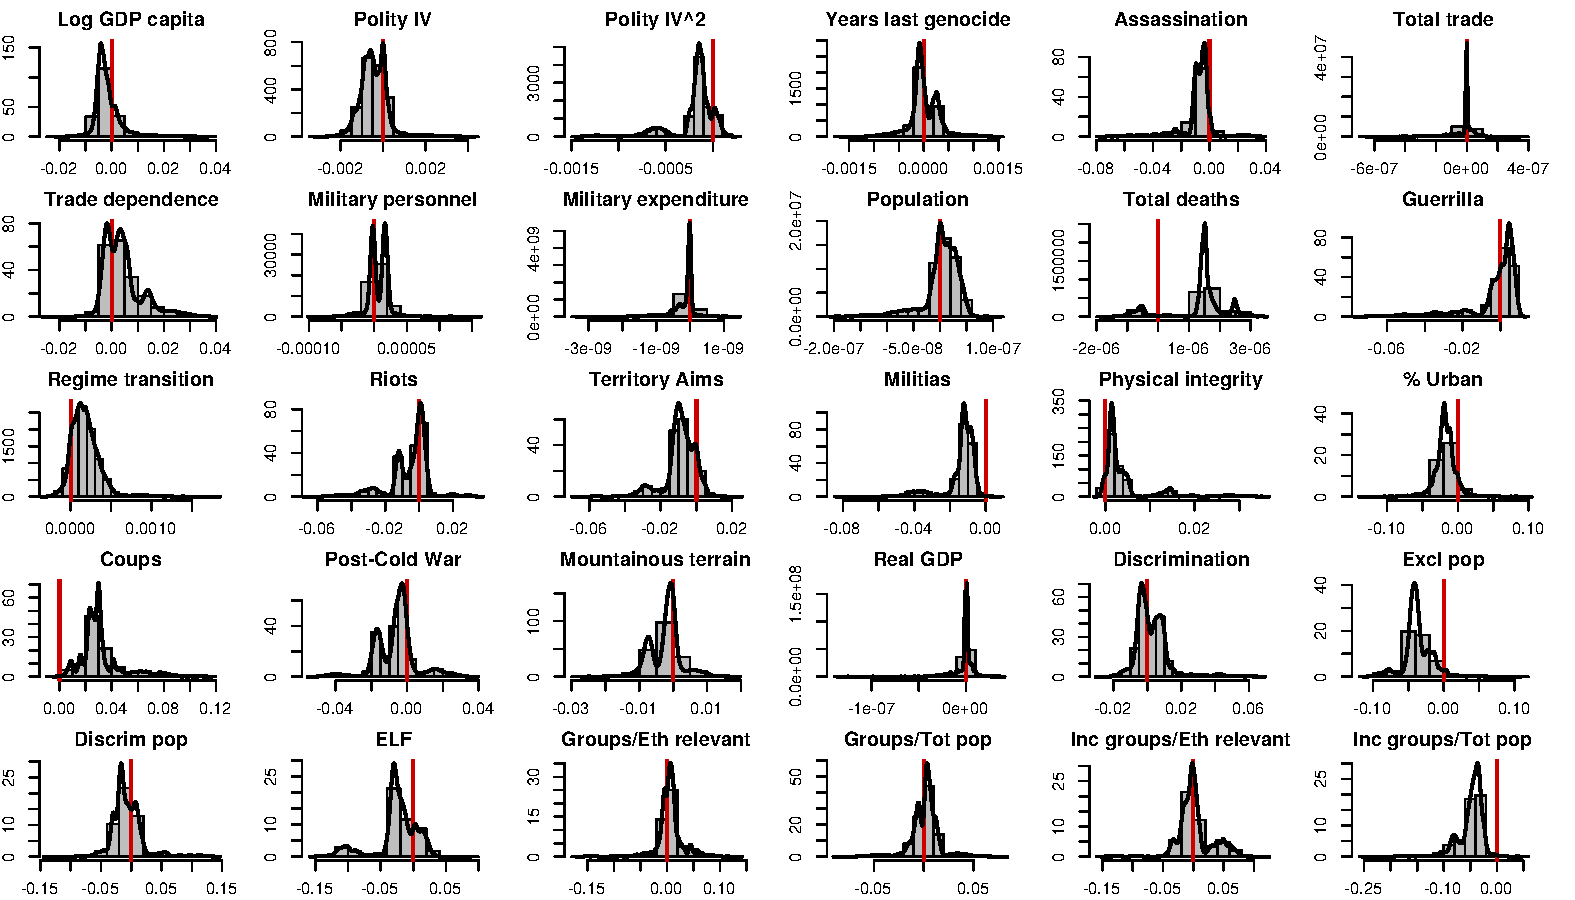
\includegraphics[width=\textwidth]{images/uamk-ucdp.pdf}
    \caption{EBA -- Genocides and Politicides during Civil Wars (UCDP Data)}
    \label{fig:uamk-ucdp}
\end{sidewaysfigure}
\clearpage

\clearpage
\begin{sidewaysfigure}
    \centering
    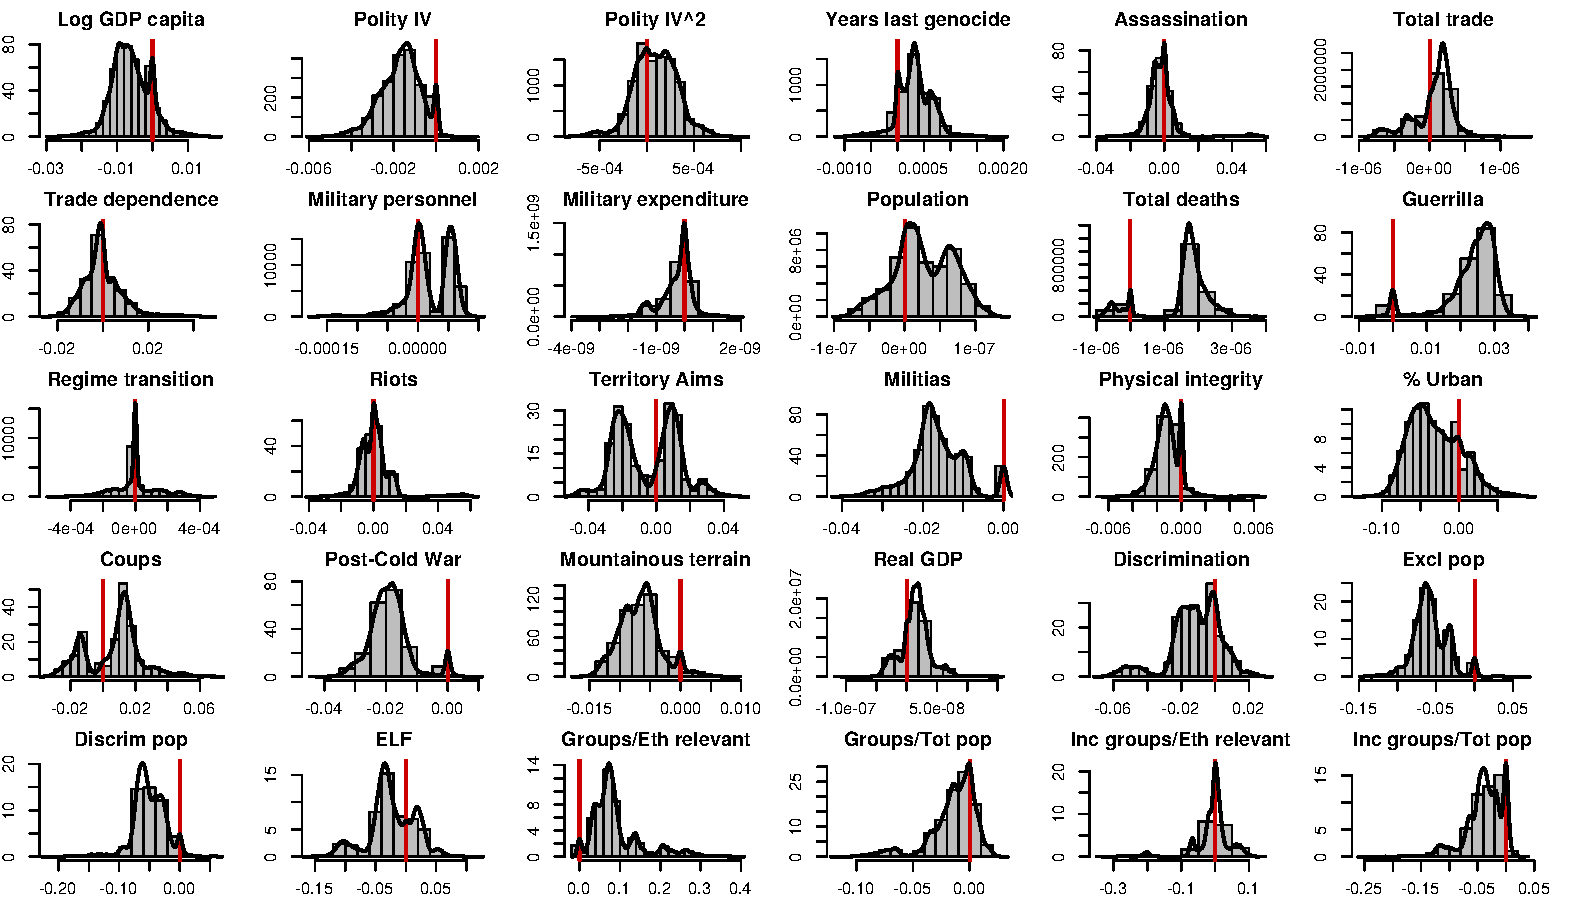
\includegraphics[width=\textwidth]{images/uamk-cow.pdf}
    \caption{EBA -- Genocides and Politicides during Civil Wars (COW Data)}
    \label{fig:uamk-cow}
\end{sidewaysfigure}
\clearpage

\clearpage
\begin{sidewaysfigure}
    \centering
    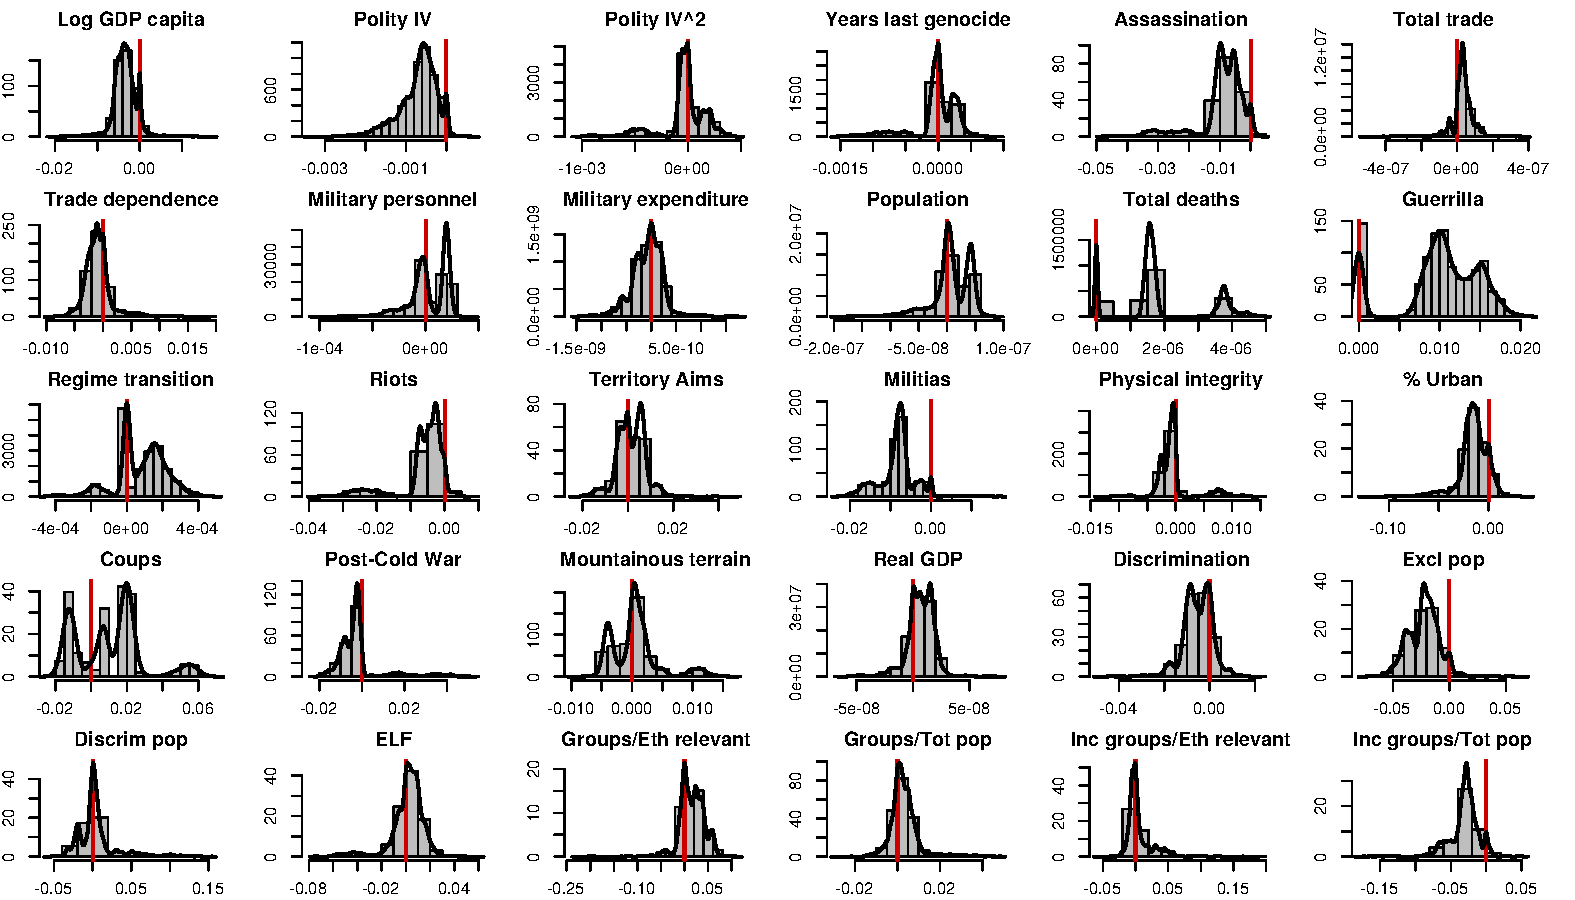
\includegraphics[width=\textwidth]{images/uamk-eth.pdf}
    \caption{EBA -- Genocides and Politicides during Ethnic Civil Wars (Cederman et al. Data)}
    \label{fig:uamk-eth}
\end{sidewaysfigure}
\clearpage


\subsection{Random Forest}
\label{sec:mk-rfe}

\subsubsection{Main Model}

We employed the \texttt{H2O} machine learning platform \citep{h2o2017} to estimate the models. \texttt{H20} is open-source, optimised for big data and estimates a large number of models with only a few lines of code. We run the algorithms on 75\% of our dataset, and use the remaining 25\% as a validation set. That is, we use a percentage of the data to assess the main model's accuracy.\footnote{For more information about training and validation samples, please refer to \href{http://docs.h2o.ai/h2o/latest-stable/h2o-docs/data-science/algo-params/validation_frame.html}{\texttt{http://docs.h2o.ai/h2o/latest-stable/h2o-docs/data-science/algo-params/validation\_frame.html}}.} Our measure of accuracy is the area under the curve (AUC). All models score well in that regard, and measures of about 0.8 accuracy in our validation sample are common.

The next two plots show the results of the main random forest models. 

\begin{figure}[H]
    \centering
    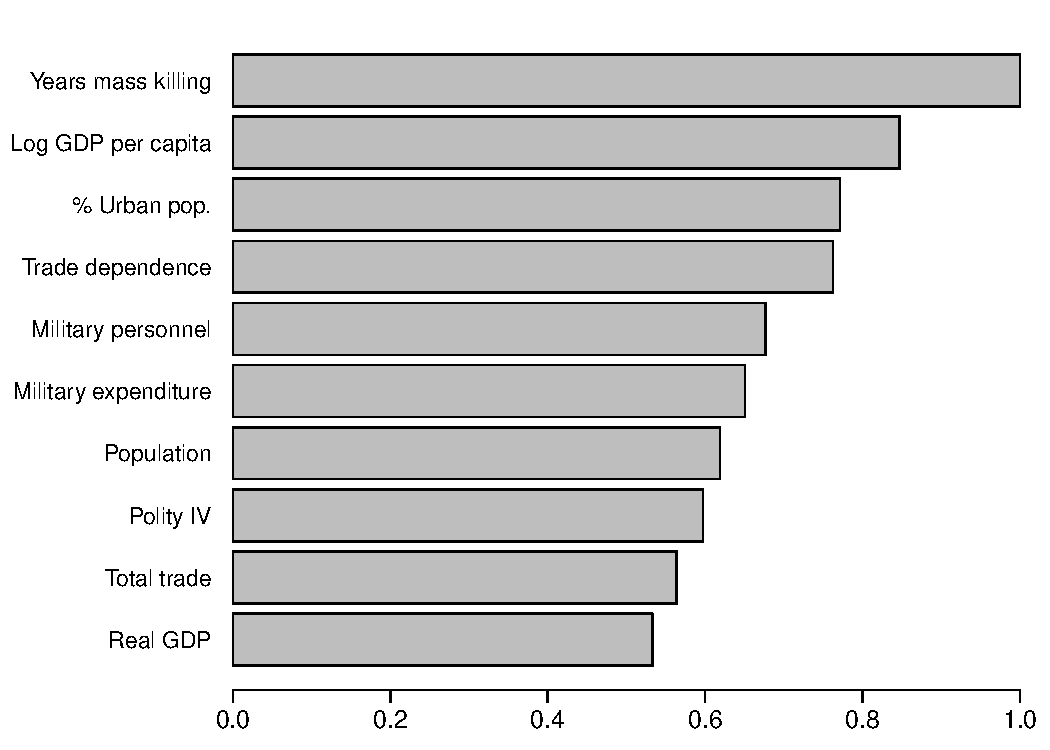
\includegraphics[width=.85\textwidth]{images/rf-mk.pdf}
    \caption{Variable Importance -- Main Model}
    \label{fig:rf-mk}
\end{figure}

\newpage 

\clearpage
\begin{sidewaysfigure}
    \centering
    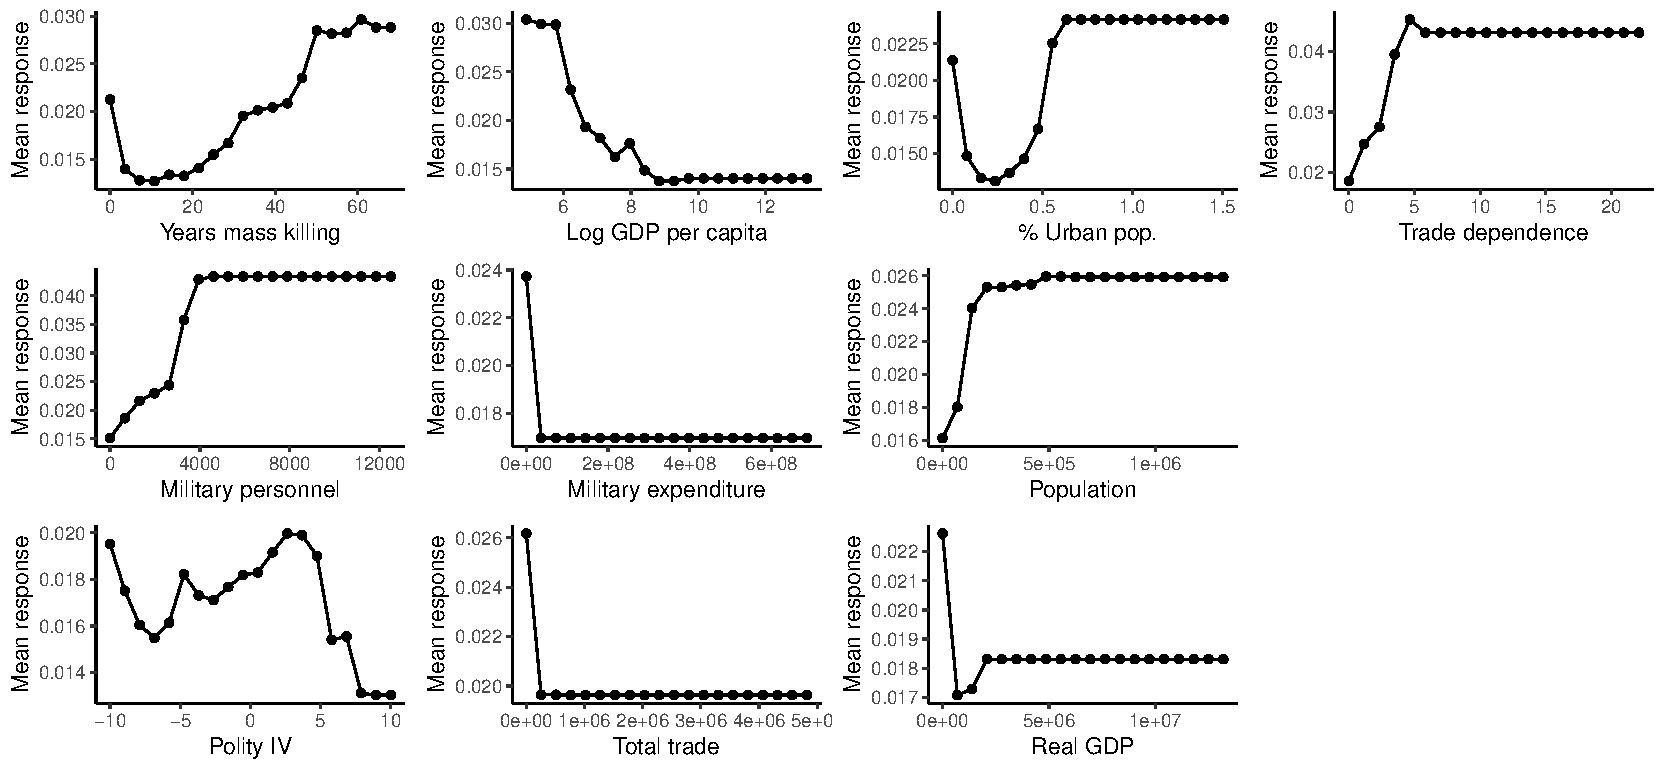
\includegraphics[width=.85\textwidth]{images/rf-mk-pd.pdf}
    \caption{Partial Dependence Plot -- Main Model}
    \label{fig:rf-mk-pd}
\end{sidewaysfigure}
\clearpage

\subsubsection{Mass Killings During Civil Wars}

The following graphs display the most important predictors of mass killings when we restrict our sample to cases that occur during civil wars. As we note in section \ref{sec:civil-wars}, we employ three different measures of civil conflicts. The first one is provided by the Uppsala Conflict Data Program \citep{allansson2017organized,gleditsch2002armed}, the second is offered by the Correlates of War \citep{sarkees2010resort}, and a third indicating the onset of ethnic conflict as coded by \citet{cederman2010ethnic}.  

\begin{figure}[H]
    \centering
    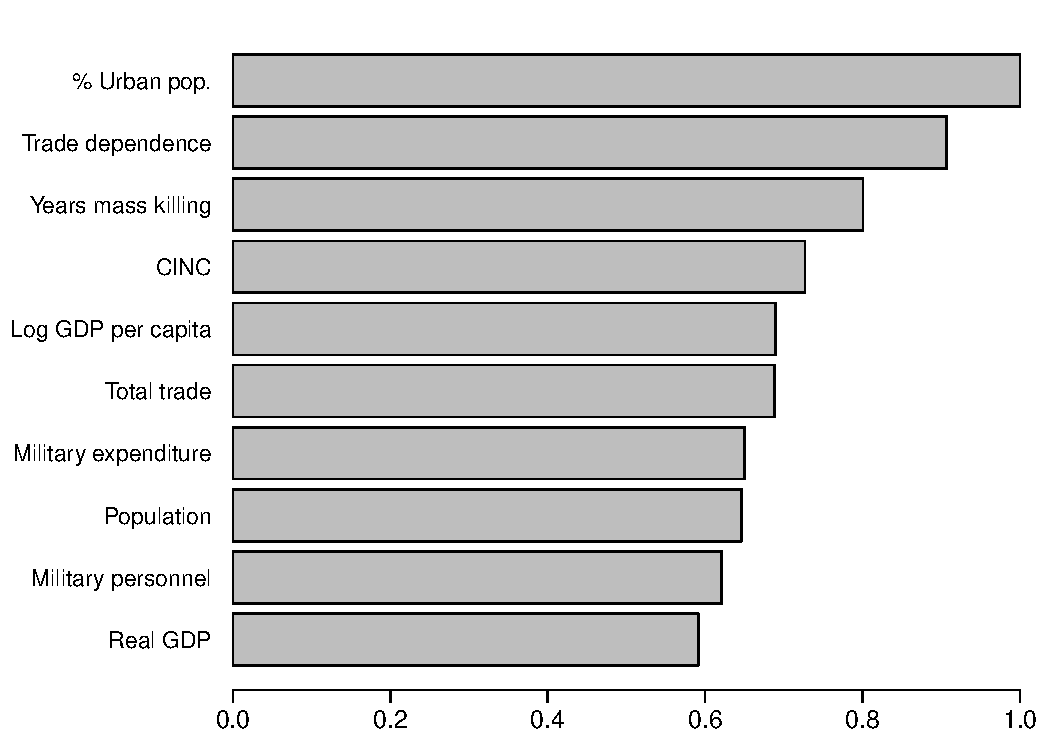
\includegraphics[width=.85\textwidth]{images/rf-ucdp.pdf}
    \caption{Variable Importance -- Mass Killings during Civil Wars (UCDP Data)}
    \label{fig:rf-mk-ucdp}
\end{figure}

\newpage 

\clearpage
\begin{sidewaysfigure}
    \centering
    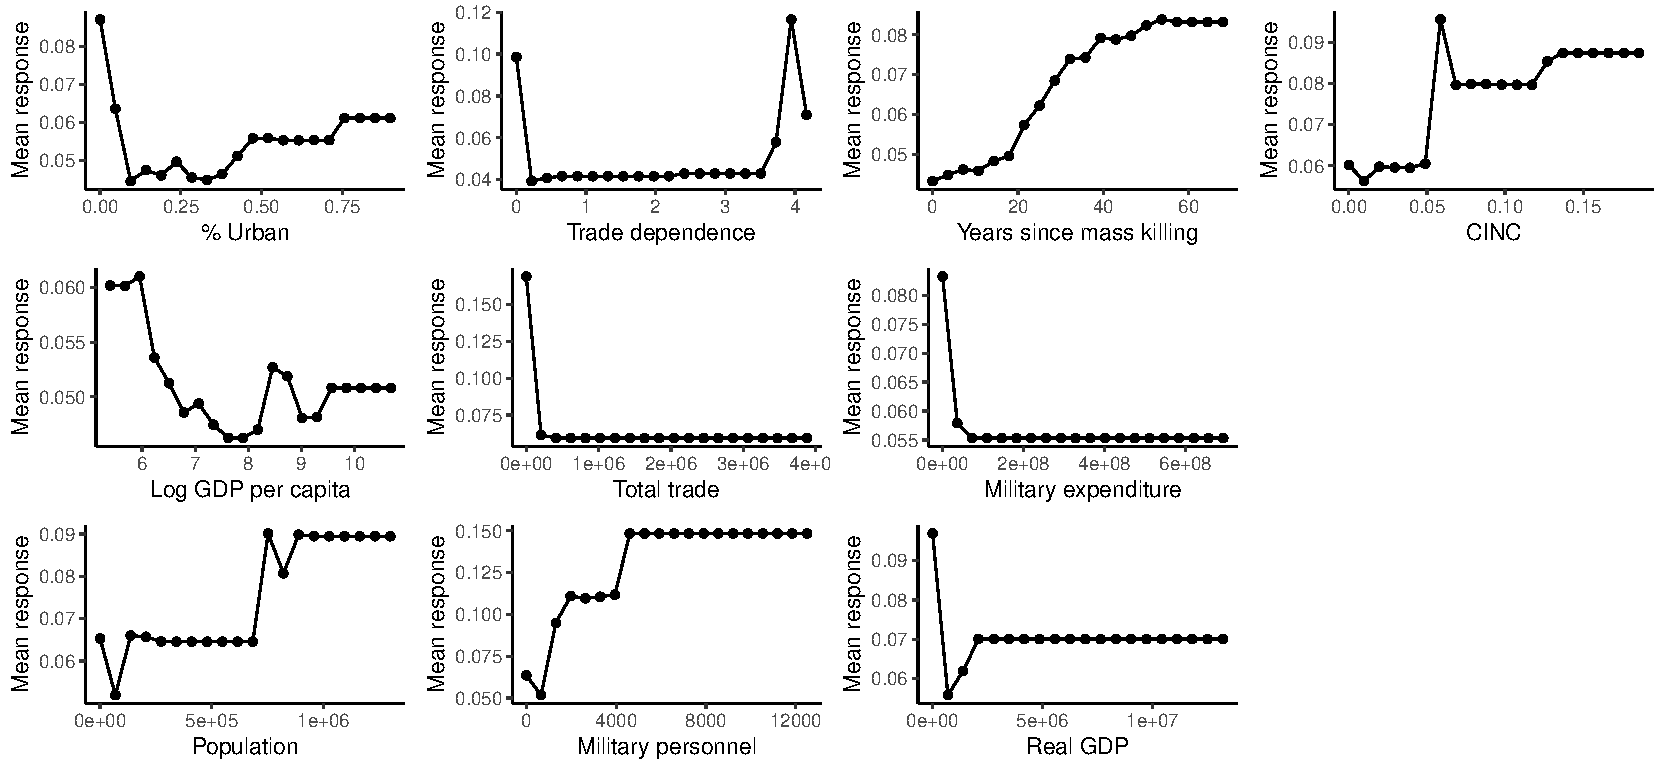
\includegraphics[width=\textwidth]{images/rf-ucdp-pd.pdf}
    \caption{Partial Dependence Plot -- Mass Killings during Civil Wars (UCDP Data)}
    \label{fig:rf-mk-ucdp-pd}
\end{sidewaysfigure}
\clearpage

\begin{figure}
    \centering
    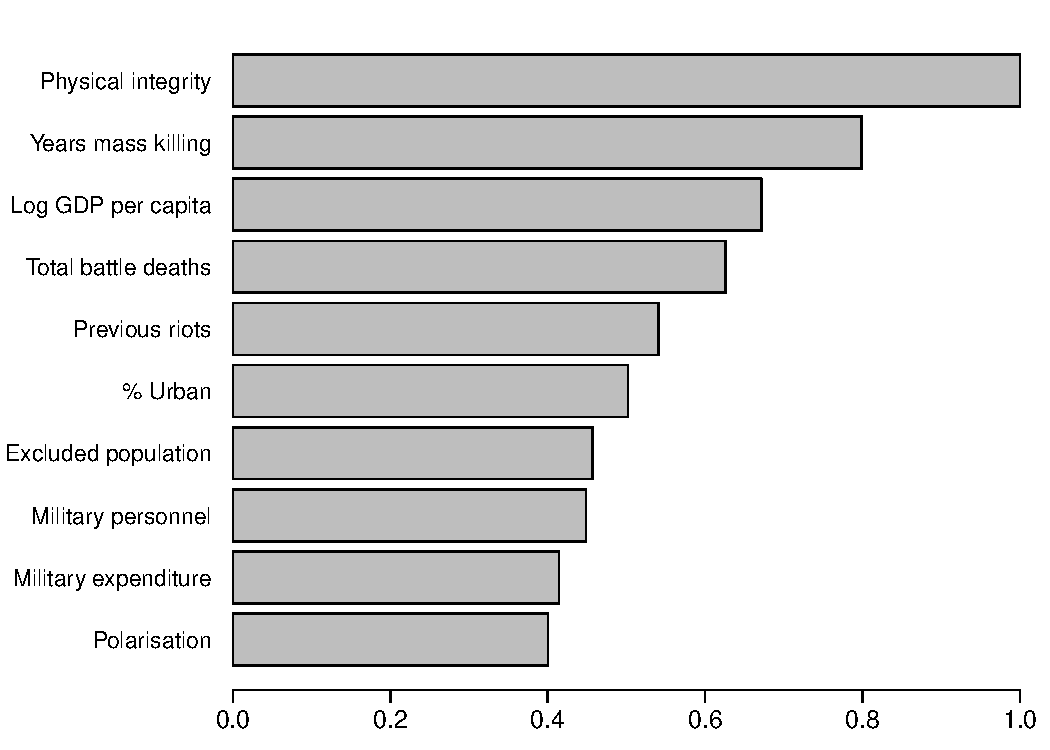
\includegraphics[width=.85\textwidth]{images/rf-cow.pdf}
    \caption{Variable Importance -- Mass Killings during Civil Wars (COW Data)}
    \label{fig:rf-mk-ucdp}
\end{figure}

\newpage 

\clearpage
\begin{sidewaysfigure}
    \centering
    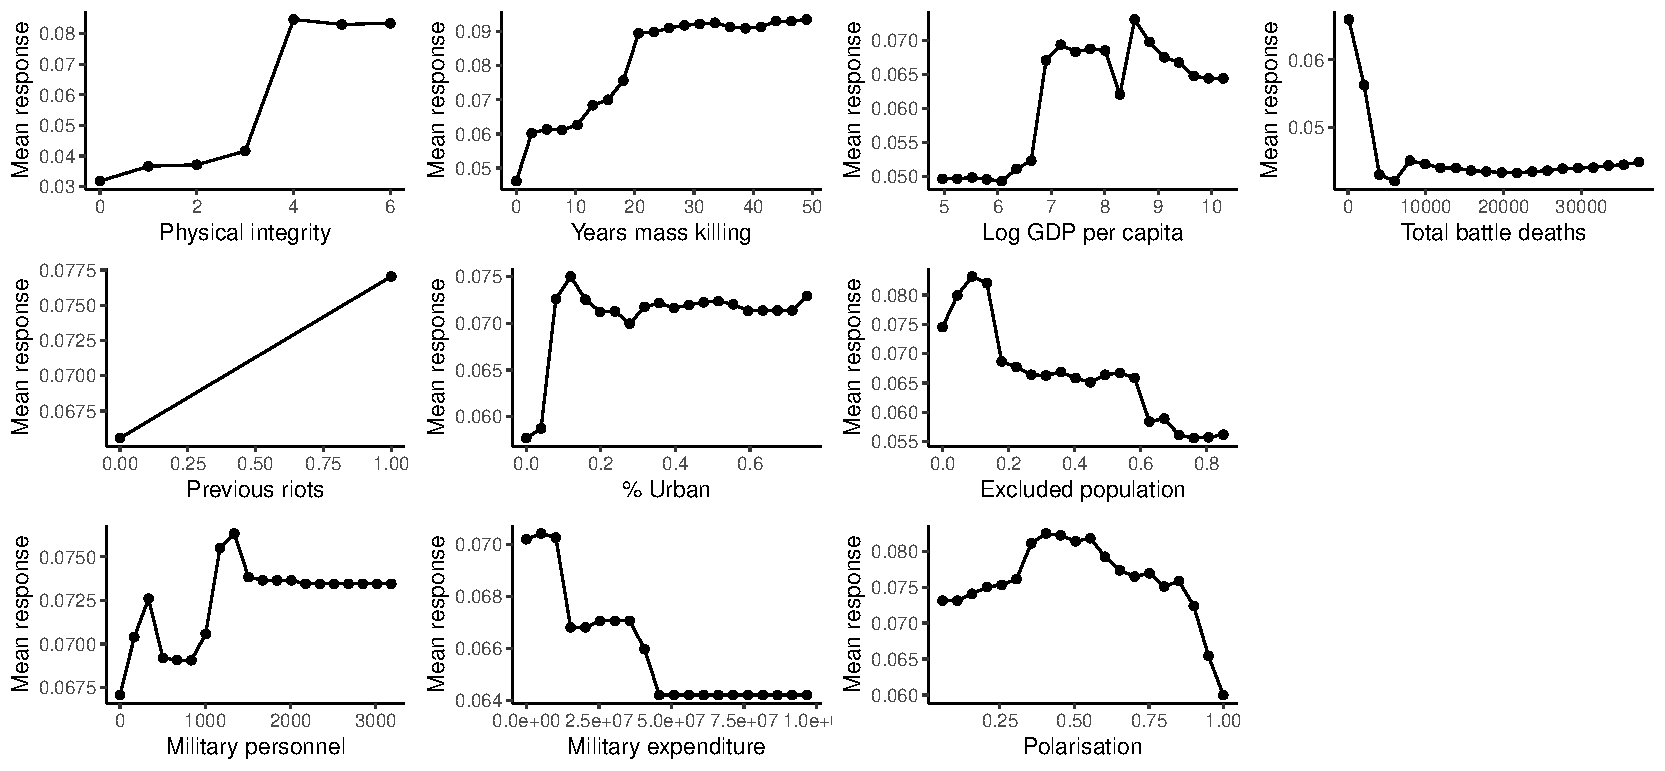
\includegraphics[width=\textwidth]{images/rf-cow-pd.pdf}
    \caption{Partial Dependence Plot -- Mass Killings during Civil Wars (COW Data)}
    \label{fig:rf-mk-ucdp-pd}
\end{sidewaysfigure}
\clearpage

\begin{figure}[H]
    \centering
    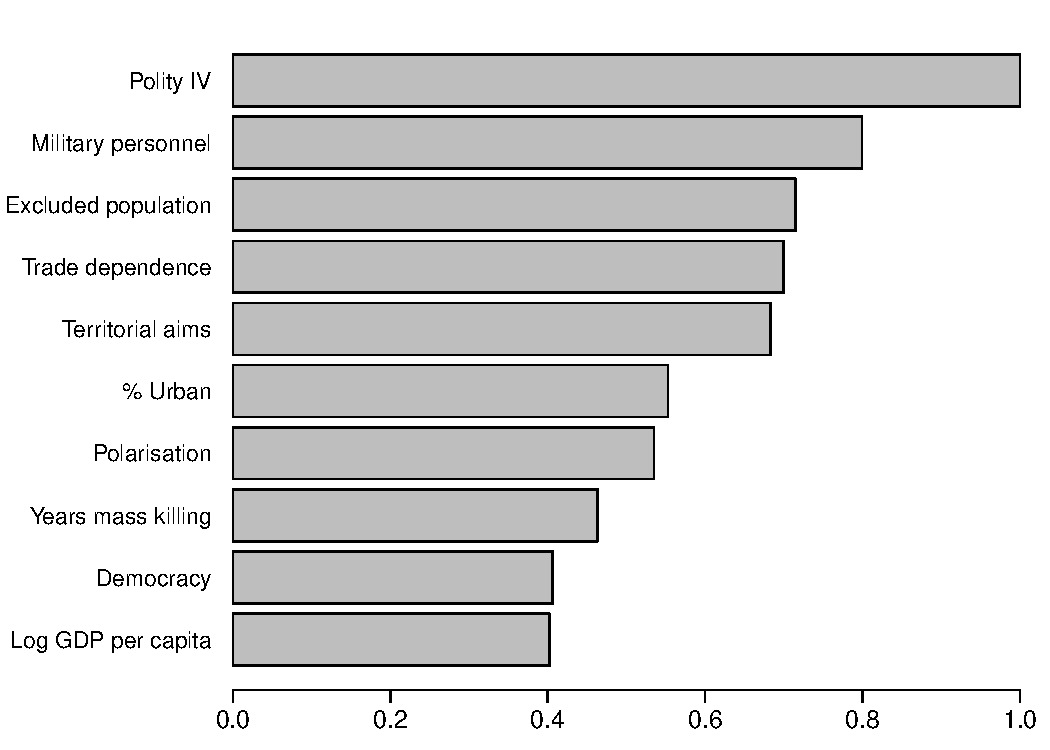
\includegraphics[width=.85\textwidth]{images/rf-eth.pdf}
    \caption{Variable Importance -- Mass Killings during Civil Wars (Cederman et al. Data)}
    \label{fig:rf-mk-ucdp}
\end{figure}

\newpage 

\clearpage
\begin{sidewaysfigure}
    \centering
    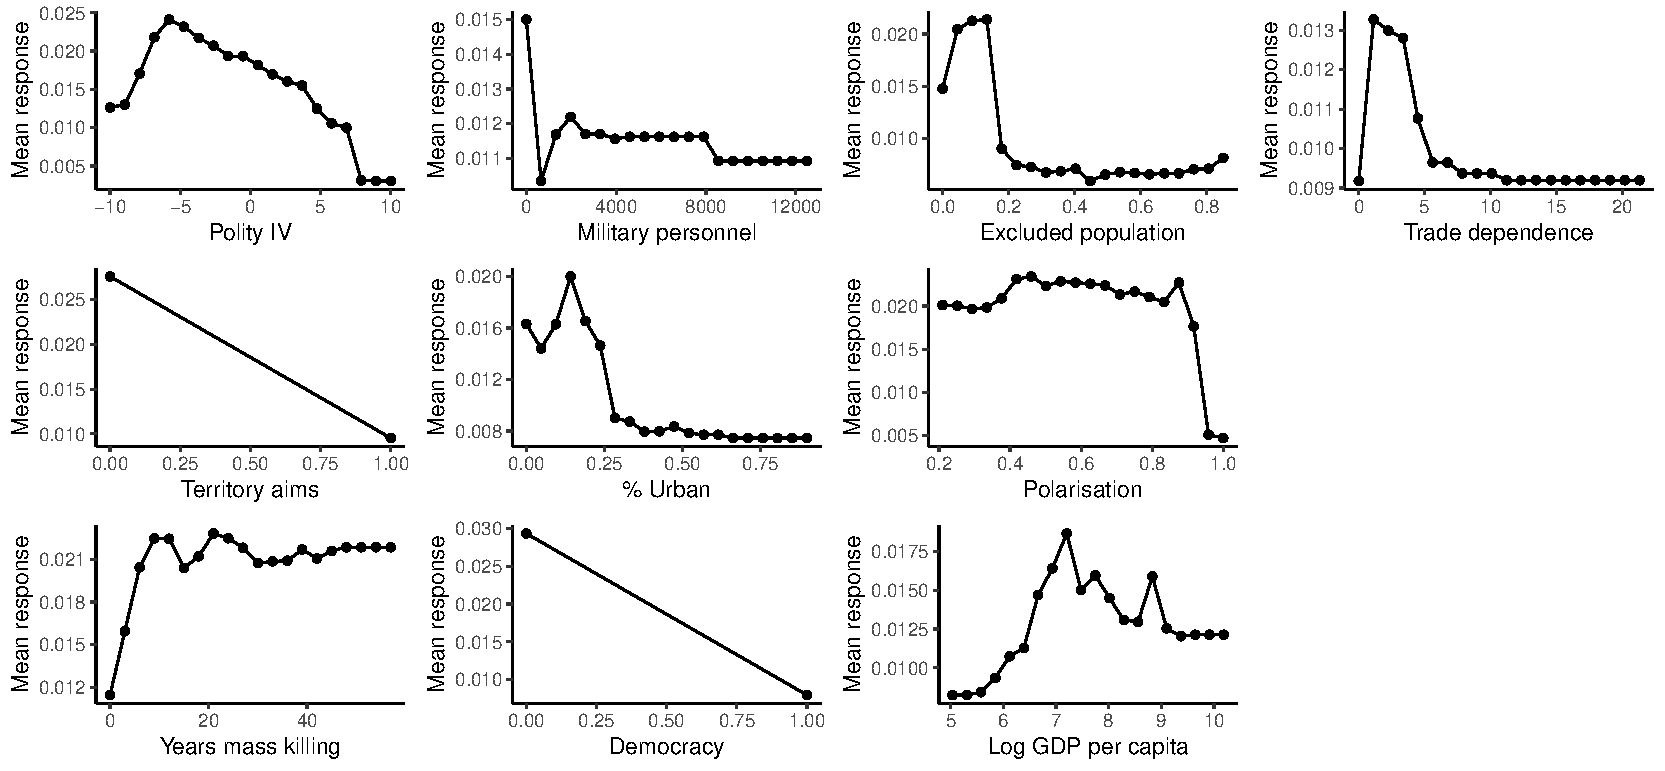
\includegraphics[width=.85\textwidth]{images/rf-eth-pd.pdf}
    \caption{Partial Dependence Plot -- Mass Killings during Civil Wars (Cederman et al. Data)}
    \label{fig:rf-mk-ucdp-pd}
\end{sidewaysfigure}
\clearpage

\newpage

\subsubsection{Alternative Random Seeds}

As random forests themselves are an approximation to a number of possible parameter combinations, changes in seed numbers may influence the model output. Thus, we start the main model with two different random seed numbers to check if the results are robust.\footnote{The numbers were generated at \href{https://www.random.org/}{\texttt{https://www.random.org/}}.} The main findings hold well; although variable importance changes from one model to another, the most significant variables appear repeatedly in the estimations. The marginal plots also show that the effect of the independent variables remain roughly similar despite the nonlinearities. The graphs below display the ten most significant predictors of mass killings and their respective partial dependence plots.

\begin{figure}[H]
    \centering
    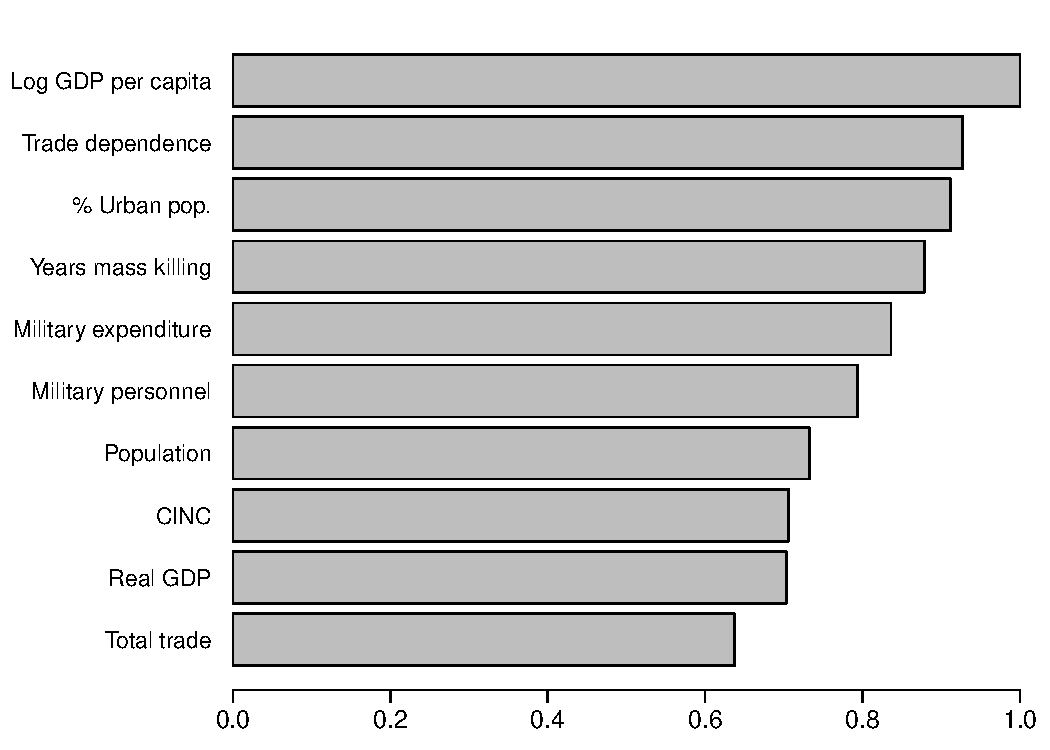
\includegraphics[width=.85\textwidth]{images/rf-mk-4363.pdf}
    \caption{Variable Importance -- Seed 4363}
    \label{fig:rf-mk-4363}
\end{figure}

\newpage

\clearpage
\begin{sidewaysfigure}
    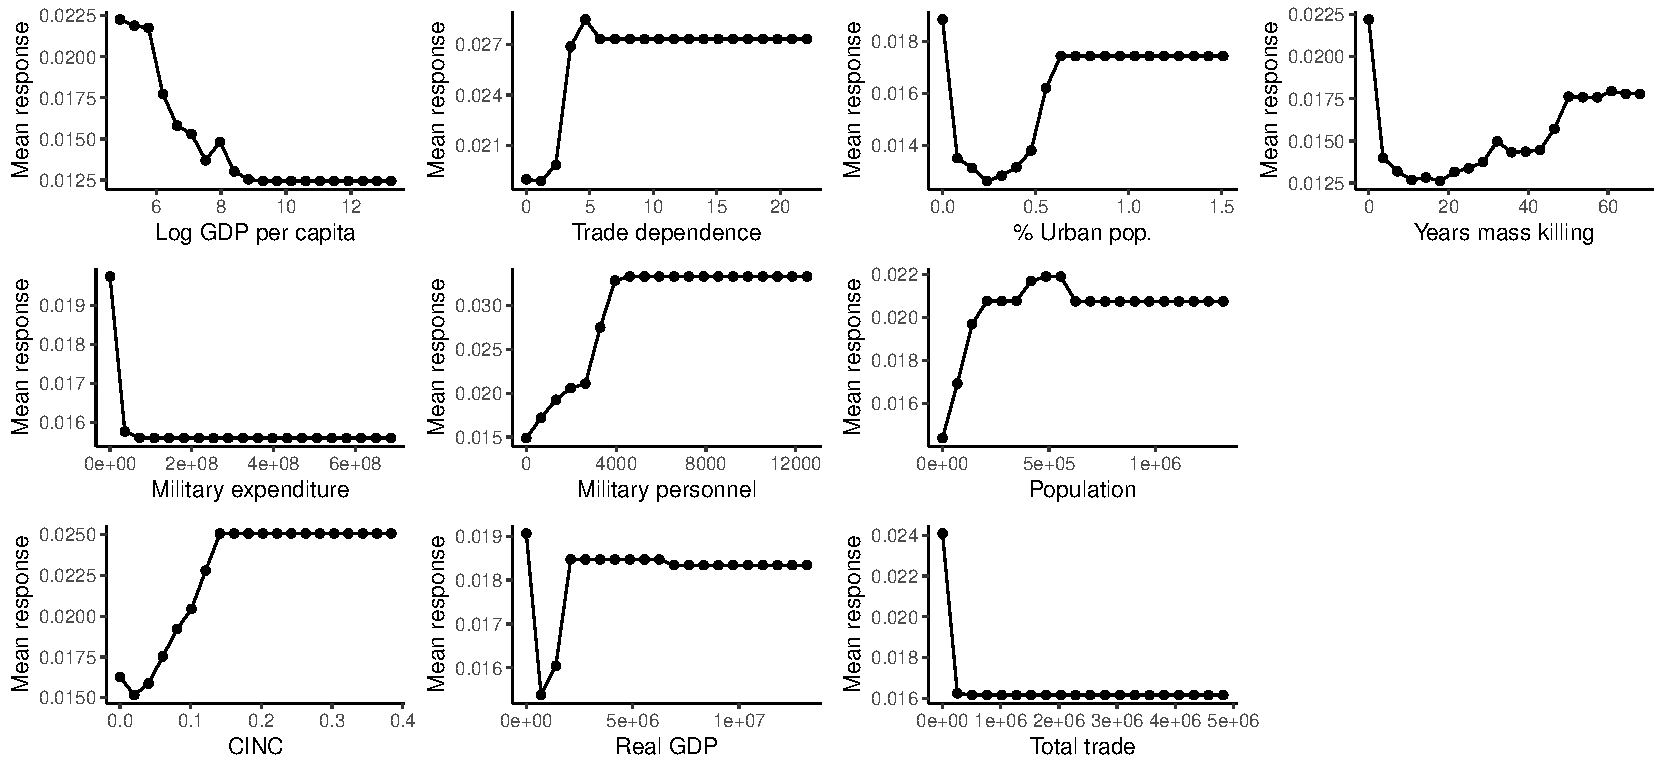
\includegraphics[width=\textheight]{images/rf-mk-4363-pd.pdf}
    \caption{Partial Dependence Plot -- Seed 4363}
    \label{fig:rf-mk-4363}
\end{sidewaysfigure}
\clearpage

\newpage


\begin{figure}
    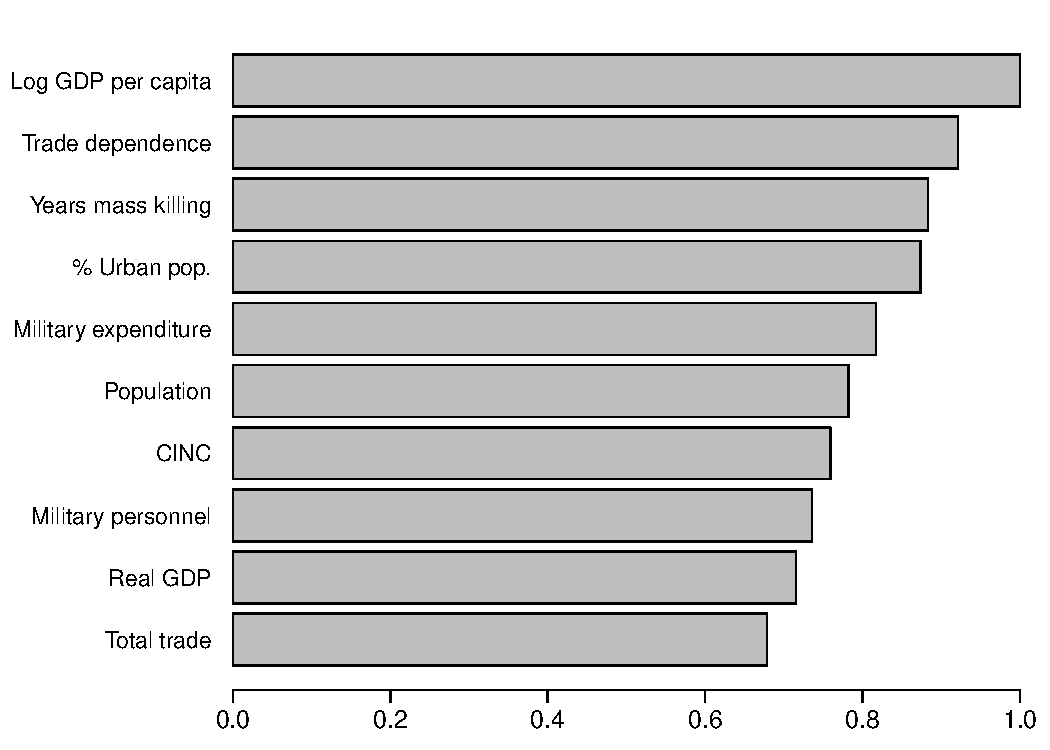
\includegraphics[width=.85\textwidth]{images/rf-mk-7015.pdf}
    \caption{Variable Importance -- Seed 7015}
    \label{fig:rf-mk-4363}
\end{figure}

\newpage

\clearpage
\begin{sidewaysfigure}
    \centering
    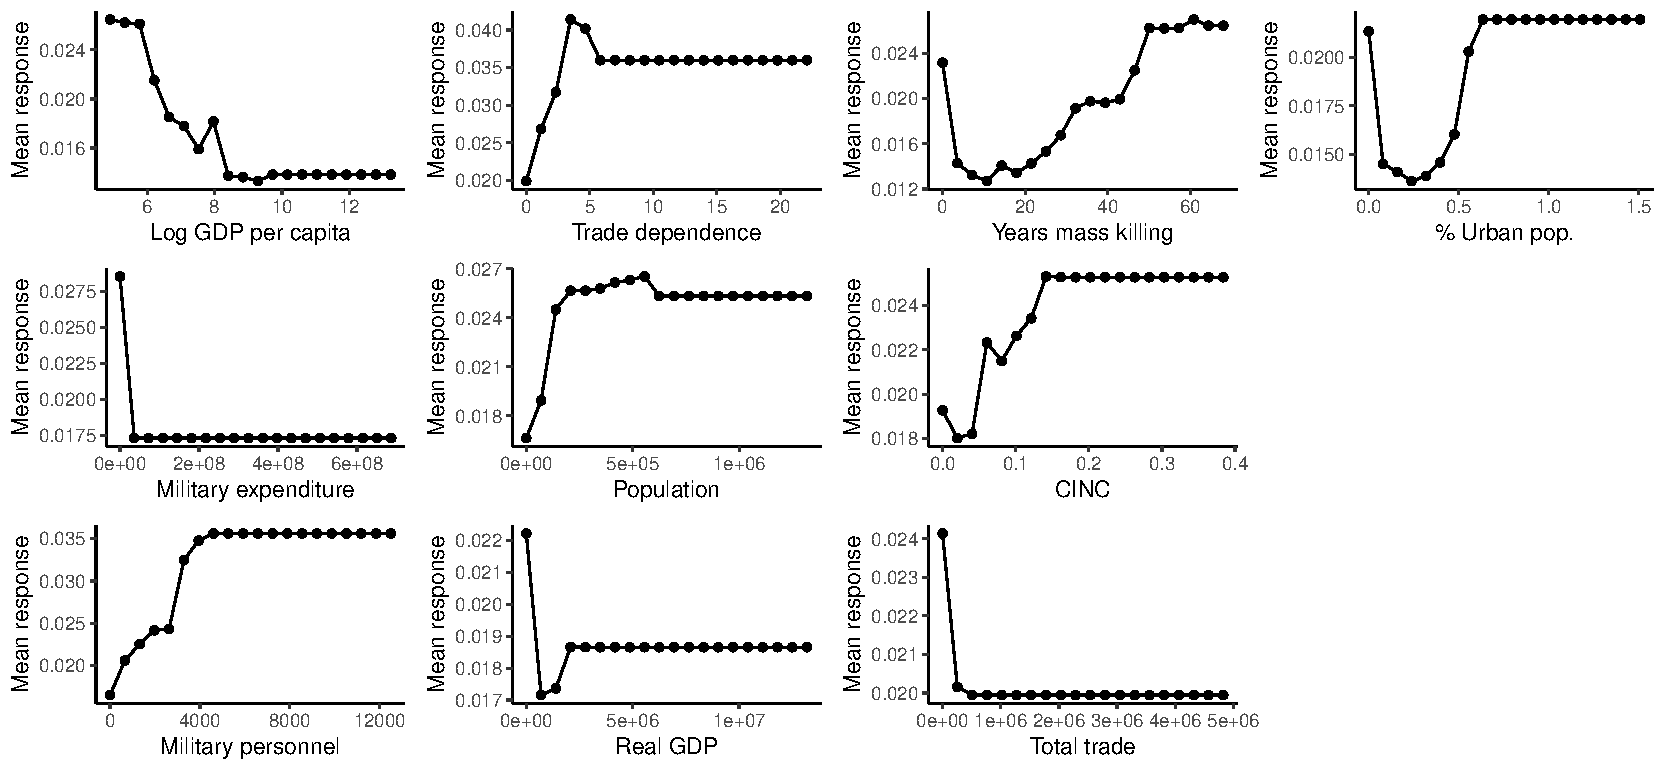
\includegraphics[width=\textwidth]{images/rf-mk-7015-pd.pdf}
    \caption{Partial Dependence Plot -- Seed 7015}
    \label{fig:rf-mk-4363}
\end{sidewaysfigure}

\newpage

\subsubsection{Mass Killings in and after the Cold War}

This last set of models splits the sample into two periods, the Cold War years and the post-Cold War years. A similar set of variables are significant in both periods, and most of them also appear in the main model shown above. 

\begin{figure}[H]
    \centering
    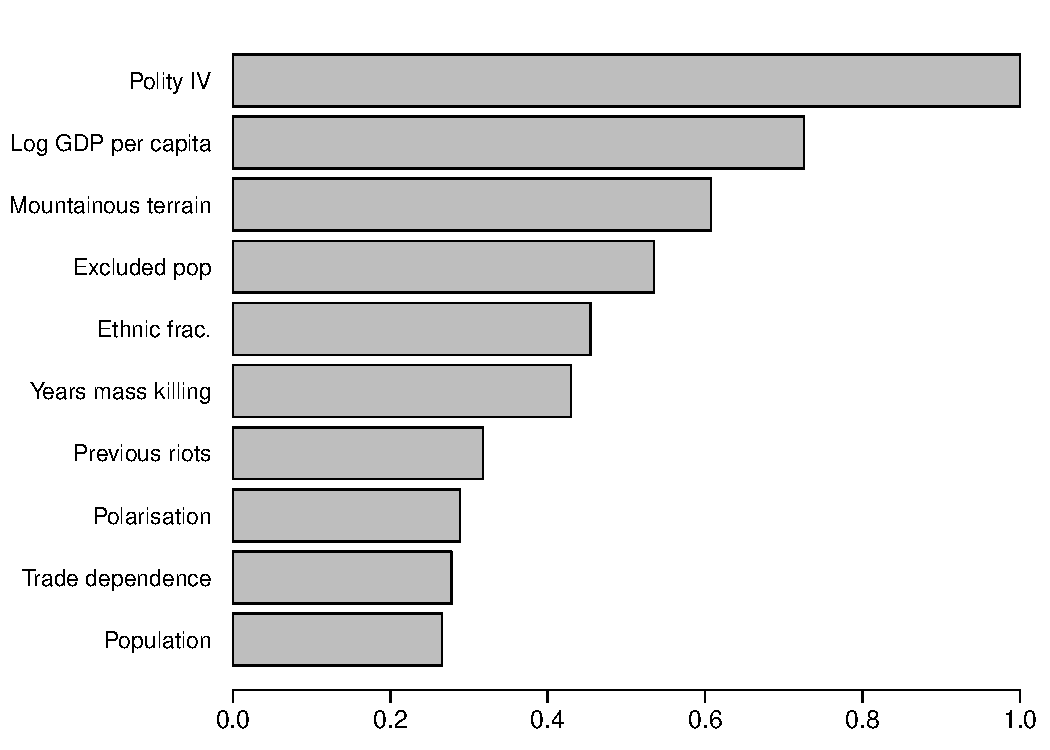
\includegraphics[width=.85\textwidth]{images/rf-coldwar.pdf}
    \caption{Variable Importance -- Cold War Period}
    \label{fig:rf-coldwar}
\end{figure}

\newpage

\clearpage
\begin{sidewaysfigure}
    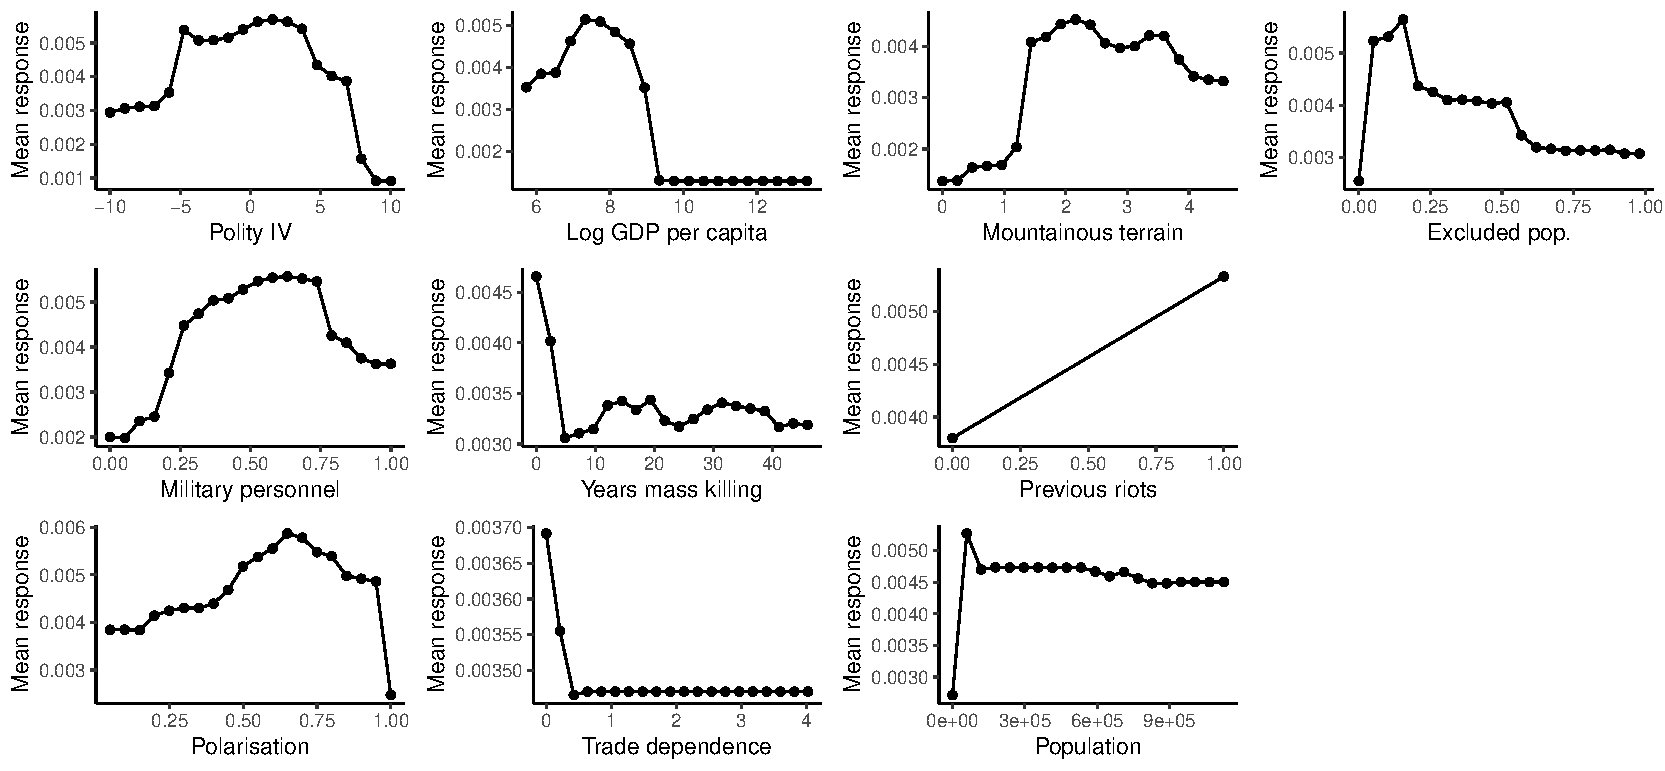
\includegraphics[width=\textwidth]{images/rf-coldwar-pd.pdf}
    \caption{Partial Dependence Plot -- Cold War Period}
    \label{fig:rf-coldwar2}
\end{sidewaysfigure}
\clearpage

\newpage

\begin{figure}[H]
    \centering
    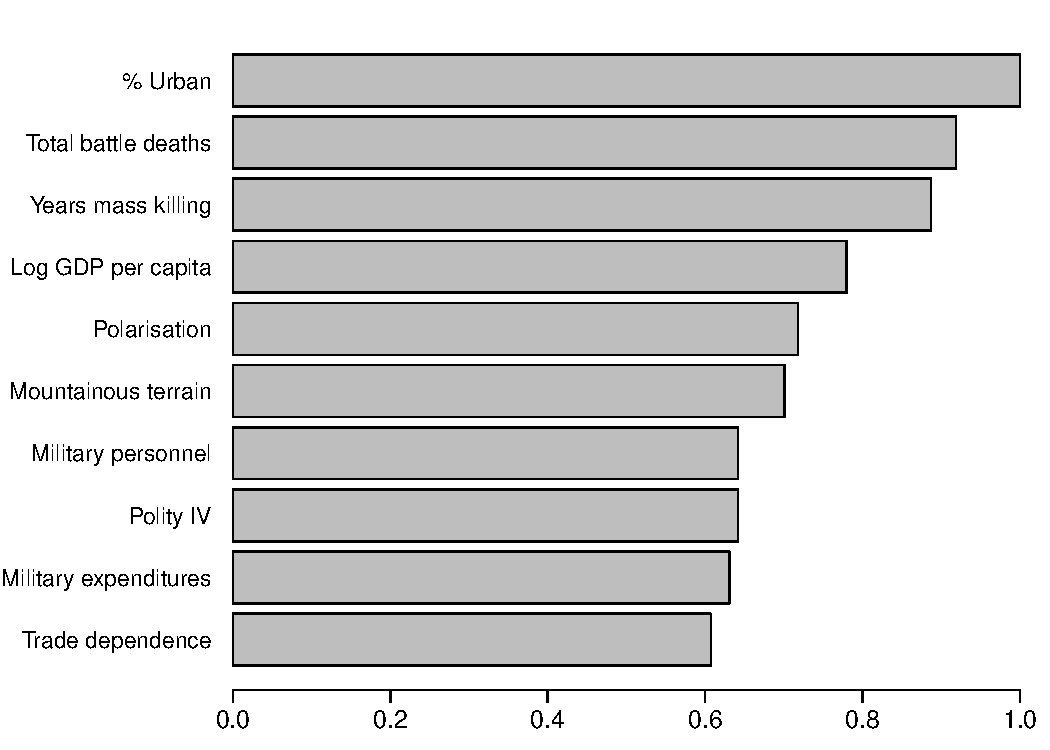
\includegraphics[width=.85\textwidth]{images/rf-postcoldwar.pdf}
    \caption{Variable Importance -- Post-Cold War Period}
    \label{fig:rf-mk-4363}
\end{figure}

\newpage

\clearpage
\begin{sidewaysfigure}
    \centering
    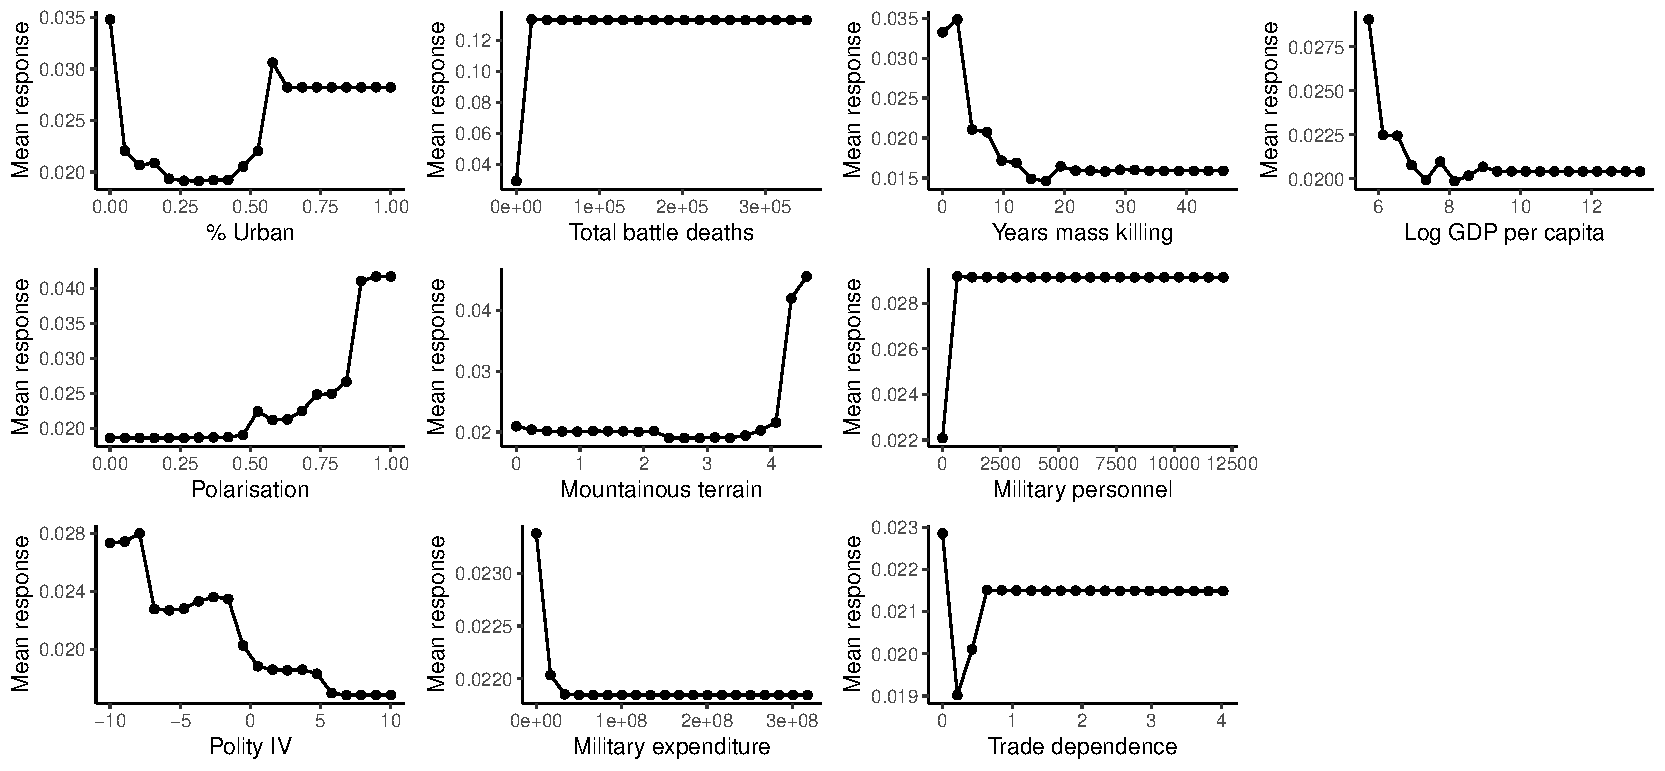
\includegraphics[width=\textwidth]{images/rf-postcoldwar-pd.pdf}
    \caption{Partial Dependence Plot -- Post-Cold War Period}
    \label{fig:rf-mk-4363}
\end{sidewaysfigure}
\clearpage

\subsubsection{Mass Killings in Peacetime}

The figures below describe the results of the random forest estimations when I restrict the sample to only peace years. All cases coded as conflicts by the UCDP, COW or Cederman and his colleagues were removed from the data, and I estimate the model only with observations where the three sourced coded as peace years. The results are almost identical to the main model, with only small variations in the importance of the explanator variables.

\begin{figure}[H]
    \centering
    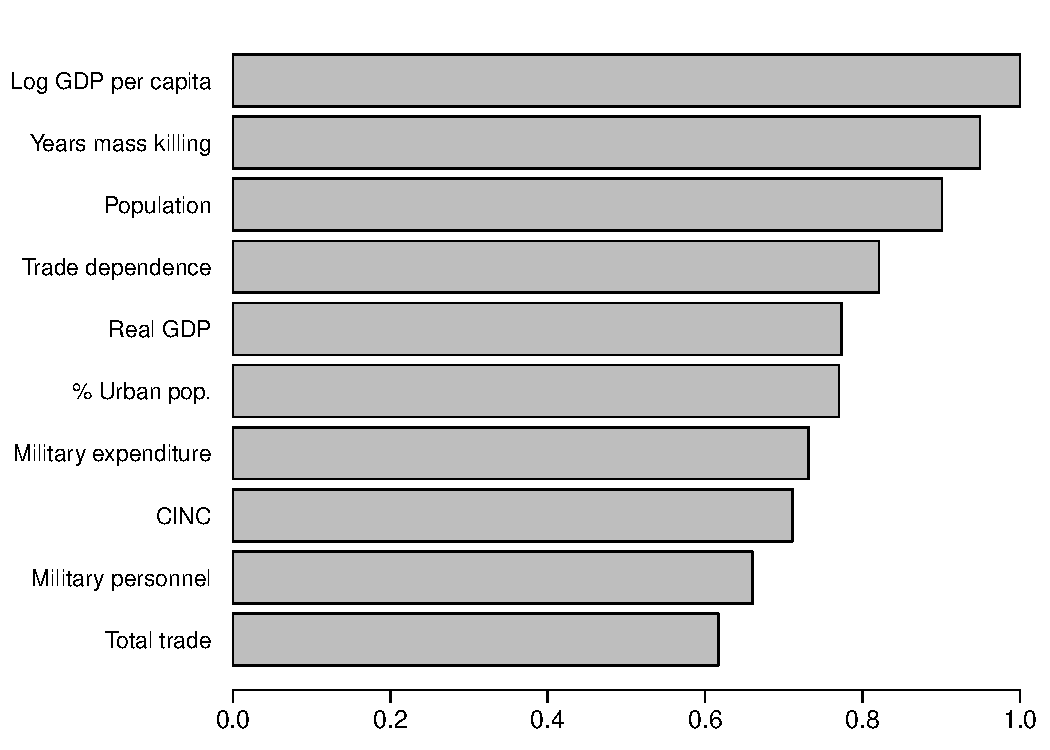
\includegraphics[width=.85\textwidth]{images/rf-nowar.pdf}
    \caption{Variable Importance -- Mass Killings during Peacetime}
    \label{fig:rf-mk-4363}
\end{figure}

\newpage

\clearpage
\begin{sidewaysfigure}
    \centering
    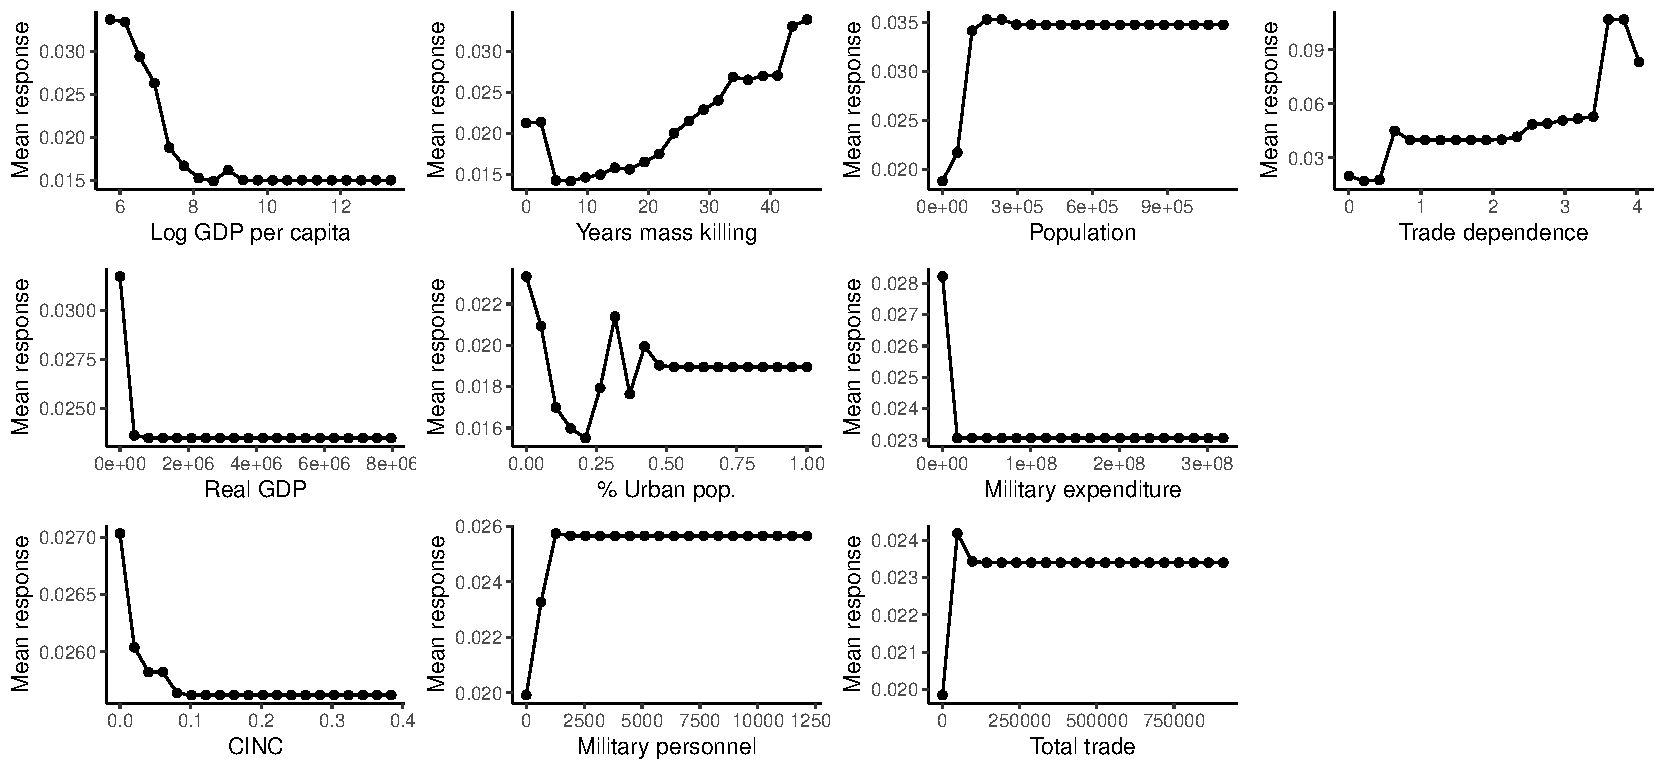
\includegraphics[width=\textwidth]{images/rf-nowar-pd.pdf}
    \caption{Partial Dependence Plot -- Mass Killings during Peacetime}
    \label{fig:rf-mk-4363}
\end{sidewaysfigure}
\clearpage


\newpage

\subsection{Harff's Genocides and Politicides Data}

\subsubsection{Main Model}

We replicate the same analysis using Harff's \citeyear{harff2003no} data. The results are comparable to the ones presented above. A similar set of variables appear in this model.

\begin{figure}[H]
    \centering
    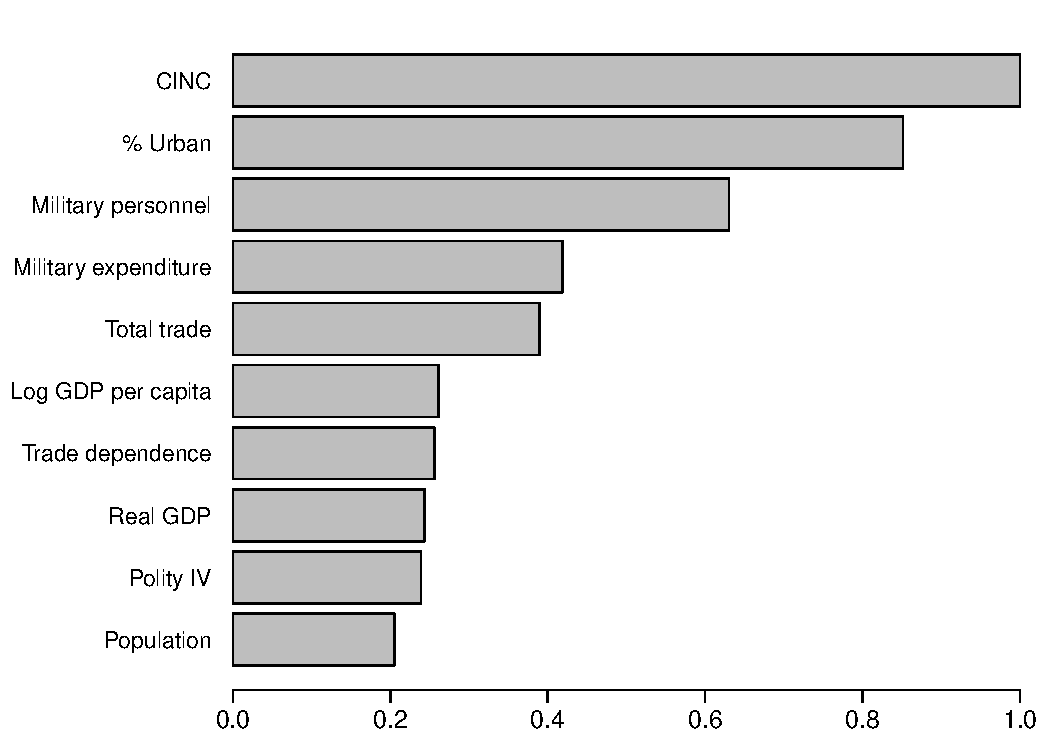
\includegraphics[width=.85\textwidth]{images/rf-uamk.pdf}
    \caption{Variable Importance -- Genocides and Politicides}
    \label{fig:rf-mk-4363}
\end{figure}

\newpage

\clearpage
\begin{sidewaysfigure}
    \centering
    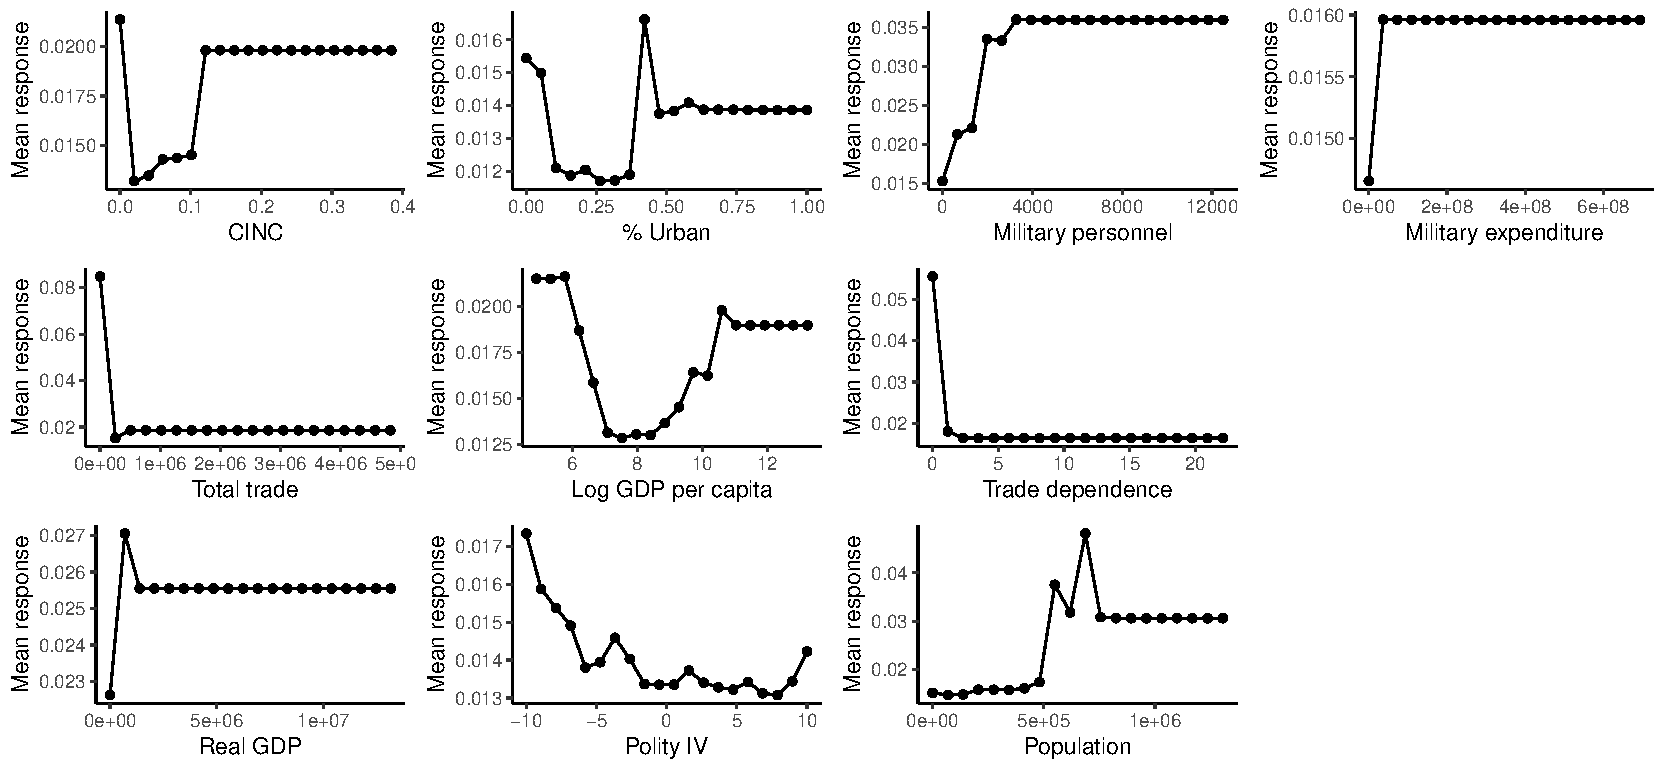
\includegraphics[width=\textwidth]{images/rf-uamk-pd.pdf}
    \caption{Partial Dependence Plot -- Genocides and Politicides}
    \label{fig:rf-mk-4363}
\end{sidewaysfigure}
\clearpage

\newpage

\subsubsection{Genocides and Politicides during Civil Wars}

Lastly, the graphs below show the results of the grid search when we only include civil war years. 

\begin{figure}[H]
    \centering
    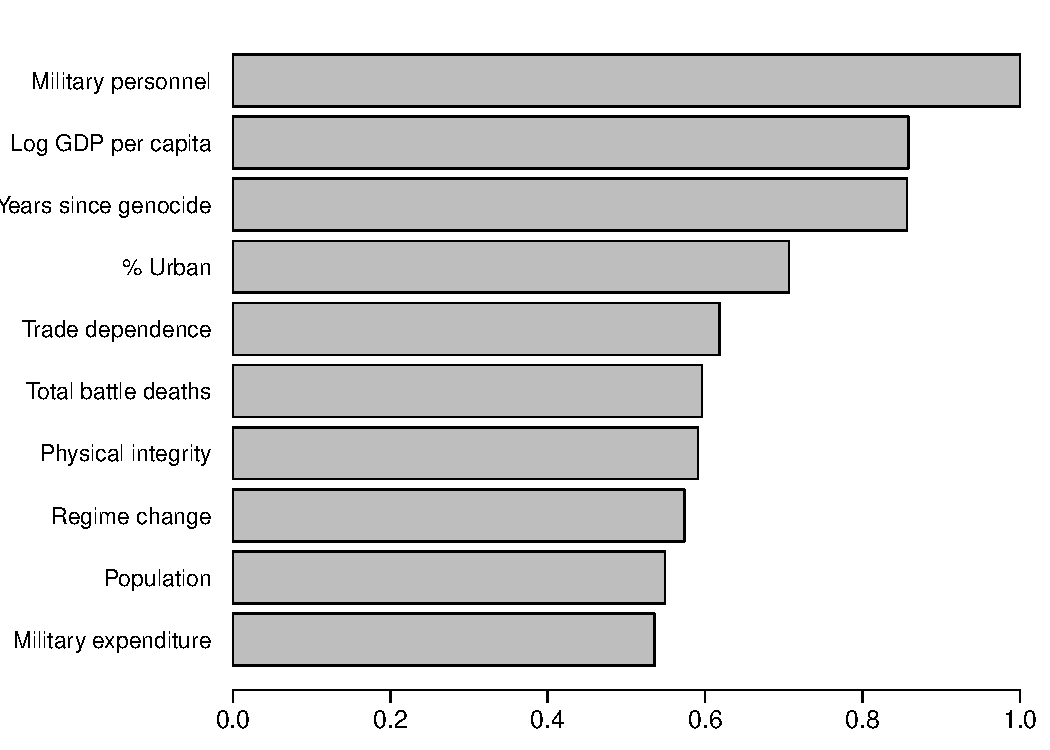
\includegraphics[width=.85\textwidth]{images/rf-uamk-ucdp.pdf}
    \caption{Variable Importance -- Genocides and Politicides during Civil Wars (UCDP Data)}
    \label{fig:rf-mk-ucdp}
\end{figure}

\newpage 

\clearpage
\begin{sidewaysfigure}
    \centering
    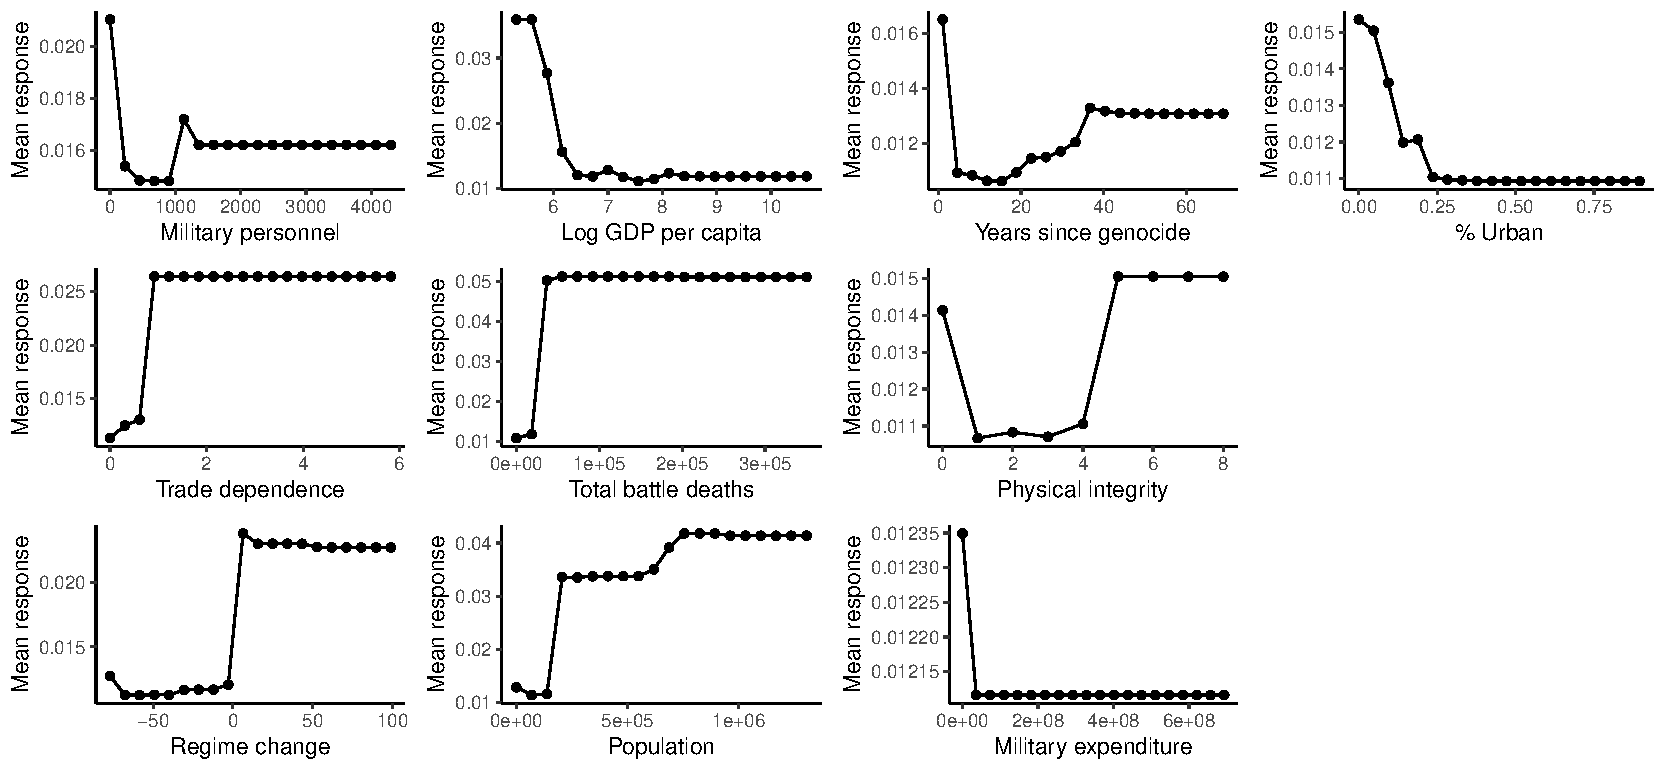
\includegraphics[width=\textwidth]{images/rf-uamk-ucdp-pd.pdf}
    \caption{Partial Dependence Plot -- Genocides and Politicides during Civil Wars (UCDP Data)}
    \label{fig:rf-mk-ucdp-pd}
\end{sidewaysfigure}
\clearpage


\begin{figure}
    \centering
    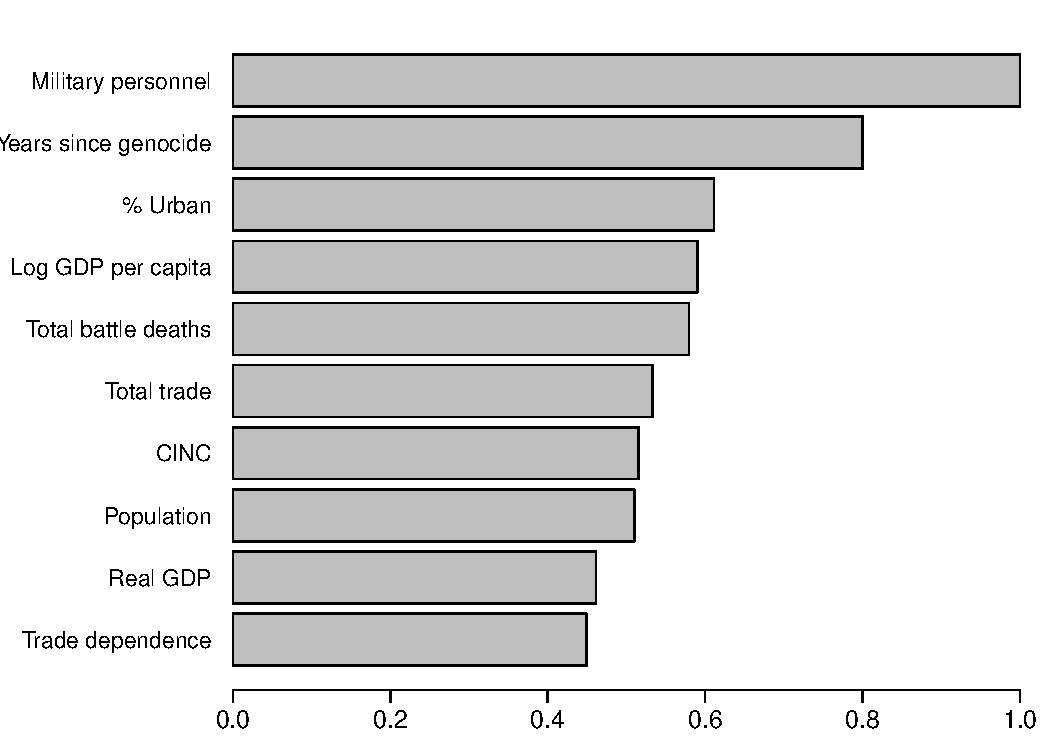
\includegraphics[width=\textwidth]{images/rf-uamk-cow.pdf}
    \caption{Variable Importance -- Genocides and Politicides during Civil Wars (COW Data)}
    \label{fig:rf-mk-ucdp}
\end{figure}

\newpage 

\clearpage
\begin{sidewaysfigure}
    \centering
    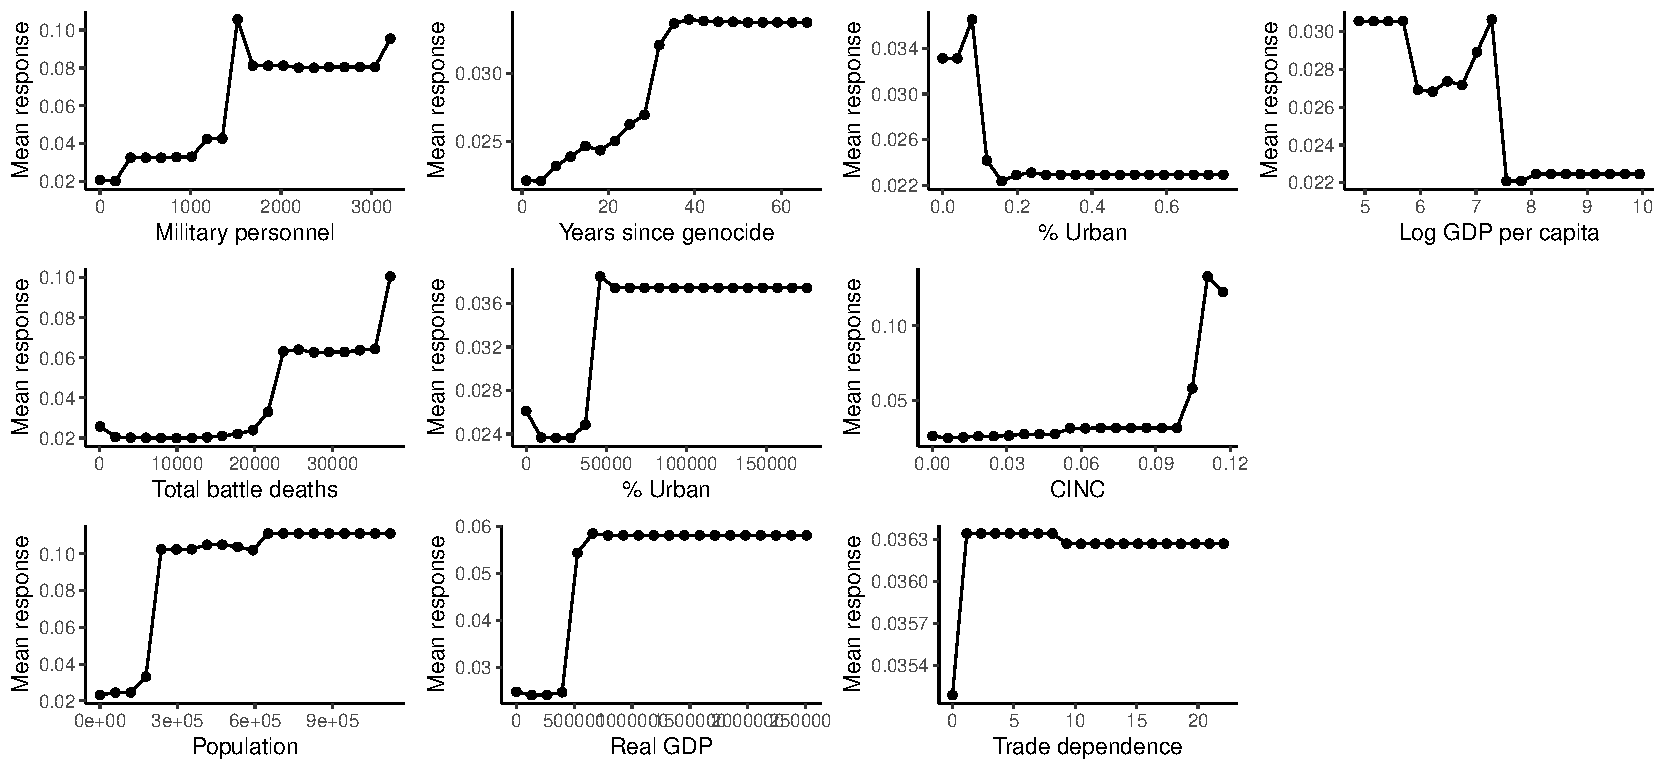
\includegraphics[width=\textwidth]{images/rf-uamk-cow-pd.pdf}
    \caption{Partial Dependence Plot -- Genocides and Politicides during Civil Wars (COW Data)}
    \label{fig:rf-mk-ucdp-pd}
\end{sidewaysfigure}
\clearpage

\begin{figure}[H]
    \centering
    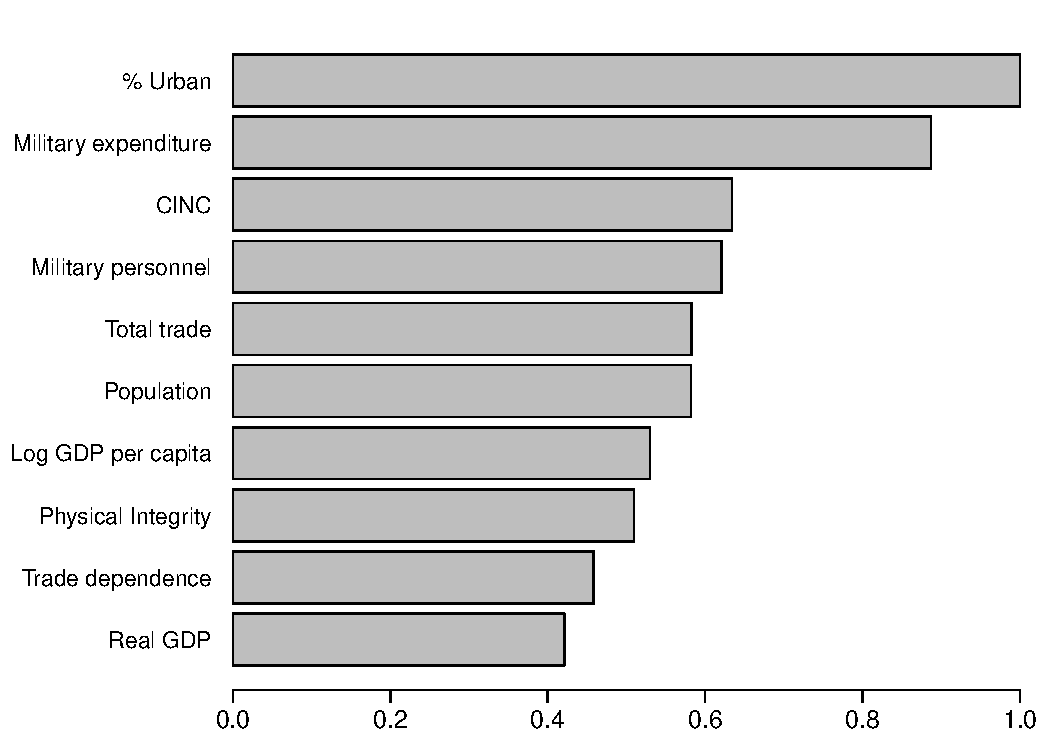
\includegraphics[width=.85\textwidth]{images/rf-uamk-eth.pdf}
    \caption{Variable Importance -- Genocides and Politicides during Civil Wars (Cederman et al. Data)}
    \label{fig:rf-mk-ucdp}
\end{figure}

\newpage 

\clearpage
\begin{sidewaysfigure}
    \centering
    \includegraphics[width=\textwidth]{images/rf-uamk-eth-pd.pdf}
    \caption{Partial Dependence Plot -- Genocides and Politicides during Civil Wars (Cederman et al. Data)}
    \label{fig:rf-mk-ucdp-pd}
\end{sidewaysfigure}
\clearpage

\subsection{\texttt{R} Code}

The \texttt{R} code below replicates all statistical analyses and graphs included in this chapter. 

\singlespacing
\small
\begin{verbatim}

#######################
### Data Wrangling ###
######################

### Load required packages
if (!require("tidyverse")) {
        install.packages("tidyverse")
}
if (!require("data.table")) {
        install.packages("data.table")
}
if (!require("ExtremeBounds")) {
        install.packages("ExtremeBounds")
}
if (!require("sandwich")) {
        install.packages("sandwich")
}
if (!require("h2o")) {
  install.packages("h2o")
}
if (!require("arm")) {
        install.packages("arm")
}

### Load data
setwd("~/Documents/GitHub/mass-killings-8k/") # set the working directory
df <- haven::read_dta("data/base variables.dta") %>% setDT()

### Select and lag variables
sd.cols <- c("UCDPcivilwarstart", "UCDPcivilwarongoing", "COWcivilwarstart",
             "COWcivilwarongoing", "ethnowarstart", "ethnowarongoing",
             "assdummy", "demdummy", "elf", "lmtnest", "pop", "realgdp",
             "rgdppc", "polity2", "exclpop", "discpop", "polrqnew",
             "poltrqnew", "egiptpolrqnew", "egippolrqnew", "discrim",
             "elf2", "interstatewar", "milex", "milper", "percentpopurban",
             "postcoldwar", "coupdummy", "riotdummy", "territoryaims",
             "totaltrade", "tradedependence", "militias", "physint", "cinc",
             "totalbeaths", "guerrilladummy", "change", "sf", "regtrans")

df1 <- cbind(df, df[, shift(.SD, 1, give.names = TRUE),
                    by = ccode, .SDcols = sd.cols]) 

# Remove the second `ccode` variable
df1 <- as.data.frame(df1[, -c(70)])

# Add new variables
df1$logrgdppc_lag_1 <- log(df1$rgdppc_lag_1)
df1$polity2sq_lag_1 <- df1$polity2_lag_1^2

# UCDP civil war == 1
df.ucdp <- df1 %>% filter(UCDPcivilwarongoing == 1)
df.ucdp <- as.data.frame(df.ucdp[, c(1:7, 76:111)])
names(df.ucdp) <- sub("_.*","", names(df.ucdp)) 

# COW civil war == 1
df.cow <- df1 %>% filter(COWcivilwarongoing == 1)
df.cow <- as.data.frame(df.cow[, c(1:7, 76:111)])
names(df.cow) <- sub("_.*","", names(df.cow)) 

# Ethnic civil war == 1
df.eth <- df1 %>% filter(ethnowarongoing == 1)
df.eth <- as.data.frame(df.eth[, c(1:7, 75:110)])
names(df.eth) <- sub("_.*","", names(df.eth)) 

# Regular model
df2 <- as.data.frame(df1[, c(1:7, 70:111)])
names(df2) <- sub("_.*","", names(df2)) 

# Cold War period
df2.coldwar <- df2 %>% filter(year <= 1991)
df2.postcoldwar <- df2 %>% filter(year > 1991)

# Countries without civil wars
df.nowar <- df2 %>% filter(COWcivilwarongoing == 0 & UCDPcivilwarongoing == 0, ethnowarongoing == 0)

#### Same procedure with the uamkstart variable

# Preparing the dataset
df3 <- haven::read_dta("data/uamkstart.dta") %>% setDT()
sd.cols <- c("UCDPcivilwarstart", "UCDPcivilwarongoing", "COWcivilwarstart",
             "COWcivilwarongoing", "ethnowarstart", "ethnowarongoing",
             "assdummy", "demdummy", "elf", "lmtnest", "pop", "realgdp",
             "rgdppc", "polity2", "exclpop", "discpop", "polrqnew",
             "poltrqnew", "egiptpolrqnew", "egippolrqnew", "discrim",
             "elf2", "interstatewar", "milex", "milper", "percentpopurban",
             "postcoldwar", "coupdummy", "riotdummy", "territoryaims",
             "totaltrade", "tradedependence", "militias", "physint", "cinc",
             "totalbeaths", "change", "guerrilladummy", "sf", "regtrans")

df4 <- cbind(df3, df3[, shift(.SD, 1, give.names = TRUE),
                    by = ccode, .SDcols = sd.cols]) 

# Remove the second `ccode` variable
df4 <- as.data.frame(df4[, -c(75)])

# Add new variables
df4$logrgdppc_lag_1 <- log(df4$rgdppc_lag_1)
df4$polity2sq_lag_1 <- df4$polity2_lag_1^2

# Renaming variables
df5 <- as.data.frame(df4[, c(1:4, 72:116)])
names(df5) <- sub("_.*","", names(df5)) 

# UCDP civil war == 1
df.ucdp2 <- df5 %>% filter(UCDPcivilwarongoing == 1)
df.ucdp2 <- as.data.frame(df.ucdp2[, c(1:7, 14:49)])
names(df.ucdp2) <- sub("_.*","", names(df.ucdp2)) 

# COW civil war == 1
df.cow2 <- df5 %>% filter(COWcivilwarongoing == 1)
df.cow2 <- as.data.frame(df.cow2[, c(1:7, 14:49)])
names(df.cow2) <- sub("_.*","", names(df.cow2)) 

# Ethnic civil war == 1
df.eth2 <- df5 %>% filter(ethnowarongoing == 1)
df.eth2 <- as.data.frame(df.eth2[, c(1:7, 14:49)])
names(df.eth2) <- sub("_.*","", names(df.eth2)) 

# Cold War period
df5.coldwar <- df5 %>% filter(year <= 1991)
df5.postcoldwar <- df5 %>% filter(year > 1991)

################################
### Extreme bounds analysis  ###
################################

# Classifying a few variables as mutually exclusive variables.
# "Change" was removed because it was correlated at 0.99 with "regtrans". 
# don't forget to add CINC
free.variables <- c("logrgdppc", "polity2", "mksyr")
civilwar.variables <- c("UCDPcivilwarongoing", "UCDPcivilwarstart",
                        "COWcivilwarongoing", "COWcivilwarstart",
                        "ethnowarongoing", "ethnowarstart")
doubtful.variables <- c("UCDPcivilwarongoing", "UCDPcivilwarstart",
                        "COWcivilwarongoing", "COWcivilwarstart",
                        "ethnowarongoing", "ethnowarstart", "assdummy",
                        "totaltrade", "tradedependence", "milper", "milex",
                        "pop", "totalbeaths", "guerrilladummy", "regtrans",
                        "riotdummy", "territoryaims", "militias",
                        "physint", "percentpopurban", "coupdummy",
                        "postcoldwar",  "lmtnest", "realgdp", "discrim",
                        "exclpop", "discpop", "elf",  "polrqnew",
                        "egippolrqnew", "poltrqnew", "egiptpolrqnew",
                        "polity2sq")

# Cluster-robust standard errors
se.clustered.robust <- function(model.object){
        model.fit <- vcovHC(model.object, type = "HC", cluster = "country")
        out <- sqrt(diag(model.fit))
        return(out)
}

### Models

# Main
m1 <- eba(y = "MKstart", free = free.variables,
          exclusive = list(civilwar.variables),
          doubtful = doubtful.variables, k = 0:4,
          data = df2, vif = 7, level = 0.9,
          se.fun = se.clustered.robust)
save(m1, file = "~/Documents/mk/mk.rda")

# 3 vars at a time
m1 <- eba(y = "MKstart", free = free.variables,
          exclusive = list(civilwar.variables),
          doubtful = doubtful.variables, k = 0:3,
          data = df2, vif = 7, level = 0.9, draws = 10000,
          se.fun = se.clustered.robust)
save(m1, file = "~/Documents/mk/mk-3vars.rda")

# 5 vars at a time
m1 <- eba(y = "MKstart", free = free.variables,
          exclusive = list(civilwar.variables),
          doubtful = doubtful.variables, k = 0:5,
          data = df2, vif = 7, draws = 50000,
          level = 0.9, se.fun = se.clustered.robust)
save(m1, file = "~/Documents/mk/mk-5vars.rda")

# Low VIF
m1 <- eba(y = "MKstart", free = free.variables,
          exclusive = list(civilwar.variables),
          doubtful = doubtful.variables, k = 0:4,
          data = df2, vif = 2.5, level = 0.9,
          draws = 50000,
          se.fun = se.clustered.robust)
save(m1, file = "~/Documents/mk/mk-low-vif.rda")

# High VIF
m1 <- eba(y = "MKstart", free = free.variables,
          exclusive = list(civilwar.variables),
          doubtful = doubtful.variables, k = 0:4,
          data = df2, vif = 10, draws = 50000,
          level = 0.9, se.fun = se.clustered.robust)
save(m1, file = "~/Documents/mk/mk-high-vif.rda")

# No VIF
m1 <- eba(y = "MKstart", free = free.variables,
          exclusive = list(civilwar.variables),
          doubtful = doubtful.variables, k = 0:4,
          data = df2, level = 0.9, draws = 50000,
          se.fun = se.clustered.robust)
save(m1, file = "~/Documents/mk/mk-no-vif.rda")

# Logit
m1 <- eba(y = "MKstart", free = free.variables,
          exclusive = list(civilwar.variables),
          doubtful = doubtful.variables, k = 0:4,
          data = df2, level = 0.9, vif = 7, draws = 50000,
          reg.fun = bayesglm, family = binomial(link = "logit"))
save(m1, file = "~/Documents/mk/mk-logit.rda")

# Probit
m1 <- eba(y = "MKstart", free = free.variables,
          exclusive = list(civilwar.variables),
          doubtful = doubtful.variables, k = 0:4,
          data = df2, level = 0.9, vif = 7, draws = 50000,
          reg.fun = bayesglm, family = binomial(link="probit"))
save(m1, file = "~/Documents/mk/mk-probit.rda")

# CINC
doubtful.variables <- c("UCDPcivilwarongoing", "UCDPcivilwarstart",
                        "COWcivilwarongoing", "COWcivilwarstart",
                        "ethnowarongoing", "ethnowarstart", "assdummy",
                        "totaltrade", "tradedependence", "cinc",
                        "totalbeaths", "guerrilladummy", "regtrans",
                        "riotdummy", "territoryaims", "militias",
                        "physint", "percentpopurban", "coupdummy",
                        "postcoldwar",  "lmtnest", "realgdp", "discrim",
                        "exclpop", "discpop", "elf",  "polrqnew",
                        "egippolrqnew", "poltrqnew", "egiptpolrqnew",
                        "polity2sq")

m1 <- eba(y = "MKstart", free = free.variables,
          exclusive = list(civilwar.variables),
          doubtful = doubtful.variables, k = 0:4,
          data = df2, vif = 7, level = 0.9, 
          se.fun = se.clustered.robust, draws = 50000)
save(m1, file = "~/Documents/mk/mk-cinc.rda")

# Cold War Period
civilwar.variables <- c("UCDPcivilwarstart","COWcivilwarstart","ethnowarstart")
m1 <- doubtful.variables <- c("UCDPcivilwarongoing", "UCDPcivilwarstart",
                              "COWcivilwarongoing", "COWcivilwarstart",
                              "ethnowarongoing", "ethnowarstart", "assdummy",
                              "totaltrade", "tradedependence", "cinc",
                              "totalbeaths", "guerrilladummy", "regtrans",
                              "riotdummy", "territoryaims", "militias",
                              "physint", "percentpopurban", "coupdummy",
                              "lmtnest", "realgdp", "discrim",
                              "exclpop", "discpop", "elf",  "polrqnew",
                              "egippolrqnew", "poltrqnew", "egiptpolrqnew",
                              "polity2sq")

m1 <- eba(y = "MKstart", free = free.variables,
          exclusive = list(civilwar.variables),
          doubtful = doubtful.variables, k = 0:4,
          data = df2.coldwar, vif = 7, level = 0.9, 
          se.fun = se.clustered.robust, draws = 50000)
save(m1, file = "data/mk-coldwar.rda")

# Post-Cold War
m1 <- doubtful.variables <- c("UCDPcivilwarongoing", "UCDPcivilwarstart",
                              "COWcivilwarongoing", "COWcivilwarstart",
                              "ethnowarongoing", "ethnowarstart", "assdummy",
                              "totaltrade", "tradedependence", "cinc",
                              "totalbeaths", "guerrilladummy", "regtrans",
                              "riotdummy", "territoryaims", "militias",
                              "physint", "percentpopurban", "coupdummy",
                              "lmtnest", "realgdp", "discrim",
                              "exclpop", "discpop", "elf",  "polrqnew",
                              "egippolrqnew", "poltrqnew", "egiptpolrqnew",
                              "polity2sq")

m1 <- eba(y = "MKstart", free = free.variables,
          exclusive = list(civilwar.variables),
          doubtful = doubtful.variables, k = 0:4,
          data = df2.postcoldwar, vif = 7, level = 0.9, 
          se.fun = se.clustered.robust, draws = 50000)
save(m1, file = "data/mk-postcoldwar.rda")

## Countries with no civil wars
free.variables <- c("logrgdppc", "polity2", "mksyr")
civilwar.variables <- c("UCDPcivilwarstart", "COWcivilwarstart",
                        "ethnowarstart")
m1 <- doubtful.variables <- c("UCDPcivilwarstart","COWcivilwarstart",
                              "ethnowarstart", "assdummy",
                              "totaltrade", "tradedependence", "cinc",
                              "totalbeaths","guerrilladummy",
                              "riotdummy", "territoryaims", "militias",
                              "physint", "percentpopurban", "coupdummy",
                              "postcoldwar", "lmtnest", "realgdp", "discrim",
                              "exclpop", "discpop", "elf",  "polrqnew",
                              "egippolrqnew", "poltrqnew", "egiptpolrqnew",
                              "polity2sq")

m1 <- eba(y = "MKstart", free = free.variables,
          exclusive = list(civilwar.variables),
          doubtful = doubtful.variables, k = 0:4,
          data = df.nowar, vif = 7, level = 0.9, 
          se.fun = se.clustered.robust, draws = 50000)
save(m1, file = "data/mk-nowar.rda")

### Ongoing Civil Wars

# UCDPcivilwarongoing == 1
doubtful.variables <- c("assdummy", "totaltrade", "tradedependence",
                        "milper", "milex", "pop", "totalbeaths",
                        "guerrilladummy", "regtrans", "riotdummy",
                        "territoryaims", "militias", "physint",
                        "percentpopurban", "coupdummy", "postcoldwar",
                        "lmtnest", "realgdp", "discrim", "exclpop",
                        "discpop", "elf",  "polrqnew", "egippolrqnew",
                        "poltrqnew", "egiptpolrqnew", "polity2sq")

m1 <- eba(y = "MKstart", free = free.variables,
          doubtful = doubtful.variables, k = 0:4,
          data = df.ucdp, vif = 7, draws = 50000,
          level = 0.9, se.fun = se.clustered.robust)
save(m1, file = "~/Documents/mk/mk-ucdp.rda")

# COWcivilwarongoing == 1
doubtful.variables <- c("assdummy", "totaltrade", "tradedependence",
                        "milper", "milex", "pop", "totalbeaths",
                        "guerrilladummy", "regtrans", "riotdummy",
                        "territoryaims", "militias", "physint",
                        "percentpopurban", "coupdummy", "postcoldwar",
                        "lmtnest", "realgdp", "discrim", "exclpop",
                        "discpop", "elf",  "polrqnew", "egippolrqnew",
                        "poltrqnew", "egiptpolrqnew", "polity2sq")

m1 <- eba(y = "MKstart", free = free.variables,
          doubtful = doubtful.variables, k = 0:4,
          data = df.cow, vif = 7, draws = 50000,
          level = 0.9, se.fun = se.clustered.robust)
save(m1, file = "~/Documents/mk/mk-cow.rda")

# Ethnic conflict == 1
doubtful.variables <- c("assdummy", "totaltrade", "tradedependence",
                        "milper", "milex", "pop", "totalbeaths",
                        "guerrilladummy", "regtrans", "riotdummy",
                        "territoryaims", "militias", "physint",
                        "percentpopurban", "coupdummy", "postcoldwar",
                        "lmtnest", "realgdp", "discrim", "exclpop", 
                        "discpop", "elf",  "polrqnew", "egippolrqnew",
                        "poltrqnew", "egiptpolrqnew", "polity2sq")

m1 <- eba(y = "MKstart", free = free.variables,
          doubtful = doubtful.variables, k = 0:4,
          data = df.eth, vif = 7, draws = 50000,
          level = 0.9, se.fun = se.clustered.robust)
save(m1, file = "~/Documents/mk/mk-eth.rda")

# Main
free.variables <- c("logrgdppc", "polity2", "uamkyr")
civilwar.variables <- c("UCDPcivilwarongoing", "UCDPcivilwarstart",
                        "COWcivilwarongoing", "COWcivilwarstart",
                        "ethnowarongoing", "ethnowarstart")
doubtful.variables <- c("UCDPcivilwarongoing", "UCDPcivilwarstart",
                        "COWcivilwarongoing", "COWcivilwarstart",
                        "ethnowarongoing", "ethnowarstart", "assdummy",
                        "totaltrade", "tradedependence", "milper", "milex",
                        "pop", "totalbeaths", "guerrilladummy", "regtrans",
                        "riotdummy", "territoryaims", "militias",
                        "physint", "percentpopurban", "coupdummy",
                        "postcoldwar",  "lmtnest", "realgdp", "discrim",
                        "exclpop", "discpop", "elf",  "polrqnew",
                        "egippolrqnew", "poltrqnew", "egiptpolrqnew",
                        "polity2sq")
m1 <- eba(y = "uamkstart", free = free.variables,
          exclusive = list(civilwar.variables),
          doubtful = doubtful.variables, k = 0:4,
          data = df5, vif = 7, level = 0.9, 
          se.fun = se.clustered.robust)
save(m1, file = "~/Documents/mk/uamk.rda")

# 3 vars at a time
m1 <- eba(y = "uamkstart", free = free.variables,
          exclusive = list(civilwar.variables),
          doubtful = doubtful.variables, k = 0:3,
          data = df5, vif = 7, level = 0.9,
          se.fun = se.clustered.robust)
save(m1, file = "~/Documents/mk/uamk-3vars.rda")

# 5 vars at a time
m1 <- eba(y = "uamkstart", free = free.variables,
          exclusive = list(civilwar.variables),
          doubtful = doubtful.variables, k = 0:5,
          data = df5, vif = 7, draws = 50000,
          level = 0.9, se.fun = se.clustered.robust)
save(m1, file = "~/Documents/mk/uamk-5vars.rda")

# Low VIF
m1 <- eba(y = "uamkstart", free = free.variables,
          exclusive = list(civilwar.variables),
          doubtful = doubtful.variables, k = 0:4,
          data = df5, vif = 2.5, level = 0.9, draws = 50000,
          se.fun = se.clustered.robust)
save(m1, file = "~/Documents/mk/uamk-low-vif.rda")

# High VIF
m1 <- eba(y = "uamkstart", free = free.variables,
          exclusive = list(civilwar.variables),
          doubtful = doubtful.variables, k = 0:4,
          data = df5, vif = 10, draws = 50000,
          level = 0.9, se.fun = se.clustered.robust)
save(m1, file = "~/Documents/mk/uamk-high-vif.rda")

# No VIF
m1 <- eba(y = "uamkstart", free = free.variables,
          exclusive = list(civilwar.variables),
          doubtful = doubtful.variables, k = 0:4,
          data = df5, level = 0.9, draws = 50000,
          se.fun = se.clustered.robust)
save(m1, file = "~/Documents/mk/uamk-no-vif.rda")

# Logit
m1 <- eba(y = "uamkstart", free = free.variables,
          exclusive = list(civilwar.variables),
          doubtful = doubtful.variables, k = 0:4,
          data = df5, level = 0.9, vif = 7, draws = 50000,
          reg.fun = bayesglm, family = binomial(link = "logit"))
save(m1, file = "~/Documents/mk/uamk-logit.rda")

# Probit
m1 <- eba(y = "uamkstart", free = free.variables,
          exclusive = list(civilwar.variables),
          doubtful = doubtful.variables, k = 0:4,
          data = df5, level = 0.9, vif = 7, draws = 50000,
          reg.fun = bayesglm, family = binomial(link="probit"))
save(m1, file = "~/Documents/mk/uamk-probit.rda")

# CINC
doubtful.variables <- c("UCDPcivilwarongoing", "UCDPcivilwarstart",
                        "COWcivilwarongoing", "COWcivilwarstart",
                        "ethnowarongoing", "ethnowarstart", "assdummy",
                        "totaltrade", "tradedependence", "cinc",
                        "totalbeaths", "guerrilladummy", "regtrans",
                        "riotdummy", "territoryaims", "militias",
                        "physint", "percentpopurban", "coupdummy",
                        "postcoldwar",  "lmtnest", "realgdp", "discrim",
                        "exclpop", "discpop", "elf",  "polrqnew",
                        "egippolrqnew", "poltrqnew", "egiptpolrqnew",
                        "polity2sq")

m1 <- eba(y = "uamkstart", free = free.variables,
          exclusive = list(civilwar.variables),
          doubtful = doubtful.variables, k = 0:4,
          data = df5, vif = 7, level = 0.9, draws = 50000,
          se.fun = se.clustered.robust)
save(m1, file = "~/Documents/mk/uamk-cinc.rda")

### Ongoing Civil Wars

# UCDPcivilwarongoing == 1
df.ucdp2 <- df5 %>% filter(UCDPcivilwarongoing == 1)
doubtful.variables <- c("assdummy", "totaltrade", "tradedependence",
                        "milper", "milex", "pop", "totalbeaths",
                        "guerrilladummy", "regtrans", "riotdummy",
                        "territoryaims", "militias", "physint",
                        "percentpopurban", "coupdummy", "postcoldwar",
                        "lmtnest", "realgdp", "discrim", "exclpop",
                        "discpop", "elf",  "polrqnew", "egippolrqnew",
                        "poltrqnew", "egiptpolrqnew", "polity2sq")

m1 <- eba(y = "uamkstart", free = free.variables,
          doubtful = doubtful.variables, k = 0:4,
          data = df.ucdp2, vif = 7, draws = 50000,
          level = 0.9, se.fun = se.clustered.robust)
save(m1, file = "~/Documents/mk/uamk-ucdp.rda")

# COWcivilwarongoing == 1
df.cow2 <- df5 %>% filter(COWcivilwarongoing == 1)
doubtful.variables <- c("assdummy", "totaltrade", "tradedependence",
                        "milper", "milex", "pop", "totalbeaths",
                        "guerrilladummy", "regtrans", "riotdummy",
                        "territoryaims", "militias", "physint",
                        "percentpopurban", "coupdummy", "postcoldwar",
                        "lmtnest", "realgdp", "discrim", "exclpop",
                        "discpop", "elf",  "polrqnew", "egippolrqnew",
                        "poltrqnew", "egiptpolrqnew", "polity2sq")

m1 <- eba(y = "uamkstart", free = free.variables,
          doubtful = doubtful.variables, k = 0:4,
          data = df.cow2, vif = 7, draws = 50000,
          level = 0.9, se.fun = se.clustered.robust)
save(m1, file = "~/Documents/mk/uamk-cow.rda")

# Ethnic conflict == 1
df.eth2 <- df5 %>% filter(ethnowarongoing == 1)
doubtful.variables <- c("assdummy", "totaltrade", "tradedependence",
                        "milper", "milex", "pop", "totalbeaths",
                        "guerrilladummy", "regtrans", "riotdummy",
                        "territoryaims", "militias", "physint",
                        "percentpopurban", "coupdummy", "postcoldwar",
                        "lmtnest", "realgdp", "discrim", "exclpop", 
                        "discpop", "elf",  "polrqnew", "egippolrqnew",
                        "poltrqnew", "egiptpolrqnew", "polity2sq")

m1 <- eba(y = "uamkstart", free = free.variables,
          doubtful = doubtful.variables, k = 0:4,
          data = df.eth2, vif = 7, draws = 50000,
          level = 0.9, se.fun = se.clustered.robust)
save(m1, file = "~/Documents/mk/uamk-eth.rda")

######################
### Random forests ###
######################

# Load required package
library(h2o)
h2o.init(nthreads = -1, max_mem_size = "6G") # change min RAM size if necessary

df2a <- as.h2o(df2)

df2a$MKstart <- as.factor(df2a$MKstart)  #encode the binary response as a factor
h2o.levels(df2a$MKstart)

# Partition the data into training, validation and test sets
splits <- h2o.splitFrame(data = df2a, 
                         ratios = 0.75, # train, validation
                         seed = 1234)  # reproducibility


train <- h2o.assign(splits[[1]], "train.hex")   
valid <- h2o.assign(splits[[2]], "valid.hex") 

y <- "MKstart"
x <- setdiff(names(df2), c(y, "ccode", "year", "rgdppc",
                           "mksyr2", "mksyr3", "sf", "country",
                           "elf2", "polity2sq")) 

##########################
### Running the models ###
##########################

rf <- h2o.grid("randomForest", x = x, y = y, training_frame = train, 
               validation_frame = valid, grid_id = "grid01",
               hyper_params = list(ntrees = c(256, 512, 1024),
                                   max_depth = c(10, 20, 40),
                                   mtries = c(5, 6, 7),
                                   balance_classes = c(TRUE, FALSE),
                                   sample_rate = c(0.5, 0.632, 0.95),
                                   col_sample_rate_per_tree = c(0.5, 0.9, 1.0),
                                   histogram_type = "RoundRobin",
                                   seed = 1234)) 

# Saving the most accurate model
rf.grid <- h2o.getGrid(grid_id = "grid01",
                       sort_by = "auc",
                       decreasing = TRUE)

rf2 <- h2o.getModel(rf.grid@model_ids[[1]])
h2o.saveModel(rf2, path = "/Users/politicaltheory/Documents/GitHub/mass-killings-8k/data/")
summary(rf2)
h2o.varimp(rf2)
varimp <- as.data.frame(h2o.varimp(rf2))
h2o.varimp_plot(rf2)

# Second model
rf <- h2o.grid("randomForest", x = x, y = y, training_frame = train, 
               validation_frame = valid, grid_id = "gridrf01b",
               hyper_params = list(ntrees = c(256, 512, 1024),
                                   max_depth = c(10, 20, 40),
                                   mtries = c(5, 6, 7),
                                   balance_classes = c(TRUE, FALSE),
                                   sample_rate = c(0.5, 0.632, 0.95),
                                   col_sample_rate_per_tree = c(0.5, 0.9, 1.0),
                                   histogram_type = "RoundRobin",
                                   seed = 4363))

# Saving the most accurate model
rf.grid <- h2o.getGrid(grid_id = "gridrf01b",
                       sort_by = "auc",
                       decreasing = TRUE)

rf2 <- h2o.getModel(rf.grid@model_ids[[1]])
h2o.saveModel(rf2, path = "/Users/politicaltheory/Documents/GitHub/mass-killings-8k/data/")
summary(rf2)
varimp <- as.data.frame(h2o.varimp(rf2))

# Third model
rf <- h2o.grid("randomForest", x = x, y = y, training_frame = train, 
               validation_frame = valid, grid_id = "gridrf01c",
               hyper_params = list(ntrees = c(256, 512, 1024),
                                   max_depth = c(10, 20, 40),
                                   mtries = c(5, 6, 7),
                                   balance_classes = c(TRUE, FALSE),
                                   sample_rate = c(0.5, 0.632, 0.95),
                                   col_sample_rate_per_tree = c(0.5, 0.9, 1.0),
                                   histogram_type = "RoundRobin",
                                   seed = 7015)) 

# Saving the most accurate model
rf.grid <- h2o.getGrid(grid_id = "gridrf01c",
                       sort_by = "auc",
                       decreasing = TRUE)

rf2 <- h2o.getModel(rf.grid@model_ids[[1]])
h2o.saveModel(rf2, path = "/Users/politicaltheory/Documents/GitHub/mass-killings-8k/data/")
summary(rf2)
varimp <- as.data.frame(h2o.varimp(rf2))
h2o.varimp_plot(rf2)

##########################
### Ongoing civil wars ###
##########################

# UCDP == 1
df.ucdpa <- as.h2o(df.ucdp)

df.ucdpa$MKstart <- as.factor(df.ucdpa$MKstart)  #encode the binary repsonse as a factor
h2o.levels(df.ucdpa$MKstart)

# Partition the data into training, validation and test sets
splits <- h2o.splitFrame(data = df.ucdpa, 
                         ratios = 0.75, 
                         seed = 1234)  


train <- h2o.assign(splits[[1]], "train.hex")   
valid <- h2o.assign(splits[[2]], "valid.hex") 

y <- "MKstart"
x <- setdiff(names(df.ucdp), c(y, "ccode", "year", "rgdppc",
                           "mksyr2", "mksyr3", "sf", "country",
                           "elf2", "polity2sq")) 

# Running the model
rf <- h2o.grid("randomForest", x = x, y = y, training_frame = train, 
               validation_frame = valid,  grid_id = "grid02",
               hyper_params = list(ntrees = c(256, 512, 1024),
                                   max_depth = c(10, 20, 40),
                                   mtries = c(5, 6, 7),
                                   balance_classes = c(TRUE, FALSE),
                                   sample_rate = c(0.5, 0.632, 0.95),
                                   col_sample_rate_per_tree = c(0.5, 0.9, 1.0),
                                   histogram_type = "RoundRobin",
                                   seed = 1234)) 

rf.grid <- h2o.getGrid(grid_id = "grid02",
                       sort_by = "auc",
                       decreasing = TRUE)
rf2 <- h2o.getModel(rf.grid@model_ids[[1]])
h2o.saveModel(rf2, path = "/Users/politicaltheory/Documents/GitHub/mass-killings-8k/data/")
summary(rf2)
h2o.varimp_plot(rf2)

# COW == 1
df.cowa <- as.h2o(df.cow)

df.cowa$MKstart <- as.factor(df.cowa$MKstart)  #encode the binary repsonse as a factor
h2o.levels(df.cowa$MKstart)

# Partition the data into training, validation and test sets
splits <- h2o.splitFrame(data = df.cowa, 
                         ratios = 0.75,  
                         seed = 1234)  


train <- h2o.assign(splits[[1]], "train.hex")   
valid <- h2o.assign(splits[[2]], "valid.hex") 

y <- "MKstart"
x <- setdiff(names(df.ucdp), c(y, "ccode", "year", "rgdppc",
                               "mksyr2", "mksyr3", "sf", "country",
                               "elf2", "polity2sq")) 

# Running the model
rf <- h2o.grid("randomForest", x = x, y = y, training_frame = train, 
               validation_frame = valid, grid_id = "gridrf03",
               hyper_params = list(ntrees = c(256, 512, 1024),
                                   max_depth = c(10, 20, 40),
                                   mtries = c(5, 6, 7),
                                   balance_classes = c(TRUE, FALSE),
                                   sample_rate = c(0.5, 0.632, 0.95),
                                   col_sample_rate_per_tree = c(0.5, 0.9, 1.0),
                                   histogram_type = "RoundRobin",
                                   seed = 1234)) 

rf.grid <- h2o.getGrid(grid_id = "gridrf03",
                       sort_by = "auc",
                       decreasing = TRUE)
rf2 <- h2o.getModel(rf.grid@model_ids[[1]])
h2o.saveModel(rf2, path = "/Users/politicaltheory/Documents/GitHub/mass-killings-8k/data/")
summary(rf2)
varimp <- as.data.frame(h2o.varimp(rf2))
h2o.varimp_plot(rf2)

# Ethnic conflict == 1
df.etha <- as.h2o(df.eth)

df.etha$MKstart <- as.factor(df.etha$MKstart)  #encode the binary repsonse as a factor
h2o.levels(df.etha$MKstart)

# Partition the data into training, validation and test sets
splits <- h2o.splitFrame(data = df.etha, 
                         ratios = 0.75,  
                         seed = 1234)  


train <- h2o.assign(splits[[1]], "train.hex")   
valid <- h2o.assign(splits[[2]], "valid.hex") 

y <- "MKstart"
x <- setdiff(names(df.eth), c(y, "ccode", "year", "rgdppc",
                               "mksyr2", "mksyr3", "sf", "country",
                               "elf2", "polity2sq")) 

# Running the model
rf <- h2o.grid("randomForest", x = x, y = y, training_frame = train, 
               validation_frame = valid, grid_id = "gridrf04",
               hyper_params = list(ntrees = c(256, 512, 1024),
                                   max_depth = c(10, 20, 40),
                                   mtries = c(5, 6, 7),
                                   balance_classes = c(TRUE, FALSE),
                                   sample_rate = c(0.5, 0.632, 0.95),
                                   col_sample_rate_per_tree = c(0.5, 0.9, 1.0),
                                   histogram_type = "RoundRobin",
                                   seed = 1234)) 

rf.grid <- h2o.getGrid(grid_id = "gridrf04",
                       sort_by = "auc",
                       decreasing = TRUE)
rf2 <- h2o.getModel(rf.grid@model_ids[[1]])
h2o.saveModel(rf2, path = "/Users/politicaltheory/Documents/GitHub/mass-killings-8k/data/")
summary(rf2)
varimp <- as.data.frame(h2o.varimp(rf2))
h2o.varimp_plot(rf2)

#######################
### Cold War Period ###
#######################
df2.coldwar2 <- as.h2o(df2.coldwar)

df2.coldwar2$MKstart <- as.factor(df2.coldwar2$MKstart)  #encode the binary repsonse as a factor
h2o.levels(df2.coldwar2$MKstart)

# Partition the data into training, validation and test sets
splits <- h2o.splitFrame(data = df2.coldwar2, 
                         ratios = 0.75,  
                         seed = 1234)  


train <- h2o.assign(splits[[1]], "train.hex")   
valid <- h2o.assign(splits[[2]], "valid.hex") 

y <- "MKstart"
x <- setdiff(names(df.eth), c(y, "ccode", "year", "rgdppc",
                              "mksyr2", "mksyr3", "sf", "country",
                              "elf2", "polity2sq")) 

rf <- h2o.grid("randomForest", x = x, y = y, training_frame = train, 
               validation_frame = valid, grid_id = "gridrf04cw",
               hyper_params = list(ntrees = c(256, 512, 1024),
                                   max_depth = c(10, 20, 40),
                                   mtries = c(5, 6, 7),
                                   balance_classes = c(TRUE, FALSE),
                                   sample_rate = c(0.5, 0.632, 0.95),
                                   col_sample_rate_per_tree = c(0.5, 0.9, 1.0),
                                   histogram_type = "RoundRobin",
                                   seed = 1234)) 

rf.grid <- h2o.getGrid(grid_id = "gridrf04cw",
                       sort_by = "auc",
                       decreasing = TRUE)
rf2 <- h2o.getModel(rf.grid@model_ids[[1]])
h2o.saveModel(rf2, path = "/Users/politicaltheory/Documents/GitHub/mass-killings-8k/data/")
summary(rf2)

############################
### Post Cold War Period ###
############################
df2.postcoldwar2 <- as.h2o(df2.postcoldwar)

df2.postcoldwar2$MKstart <- as.factor(df2.postcoldwar2$MKstart)  #encode the binary repsonse as a factor
h2o.levels(df2.postcoldwar2$MKstart)

# Partition the data into training, validation and test sets
splits <- h2o.splitFrame(data = df2.postcoldwar2, 
                         ratios = 0.75,  
                         seed = 1234)  


train <- h2o.assign(splits[[1]], "train.hex")   
valid <- h2o.assign(splits[[2]], "valid.hex") 

y <- "MKstart"
x <- setdiff(names(df.eth), c(y, "ccode", "year", "rgdppc",
                              "mksyr2", "mksyr3", "sf", "country",
                              "elf2", "polity2sq")) 

rf <- h2o.grid("randomForest", x = x, y = y, training_frame = train, 
               validation_frame = valid, grid_id = "gridrf04pcw",
               hyper_params = list(ntrees = c(256, 512, 1024),
                                   max_depth = c(10, 20, 40),
                                   mtries = c(5, 6, 7),
                                   balance_classes = c(TRUE, FALSE),
                                   sample_rate = c(0.5, 0.632, 0.95),
                                   col_sample_rate_per_tree = c(0.5, 0.9, 1.0),
                                   histogram_type = "RoundRobin",
                                   seed = 1234)) 

rf.grid <- h2o.getGrid(grid_id = "gridrf04pcw",
                       sort_by = "auc",
                       decreasing = TRUE)
rf2 <- h2o.getModel(rf.grid@model_ids[[1]])
h2o.saveModel(rf2, path = "/Users/politicaltheory/Documents/GitHub/mass-killings-8k/data/")
summary(rf2)

########################
### Only Peace Years ###
########################
df2.nowar <- as.h2o(df.nowar)

df2.nowar$MKstart <- as.factor(df2.nowar$MKstart)  #encode the binary repsonse as a factor
h2o.levels(df2.nowar$MKstart)

# Partition the data into training, validation and test sets
splits <- h2o.splitFrame(data = df2.nowar, 
                         ratios = 0.75,  
                         seed = 1234)  


train <- h2o.assign(splits[[1]], "train.hex")   
valid <- h2o.assign(splits[[2]], "valid.hex") 

y <- "MKstart"
x <- setdiff(names(df.eth), c(y, "ccode", "year", "rgdppc",
                              "mksyr2", "mksyr3", "sf", "country",
                              "elf2", "polity2sq")) 

rf <- h2o.grid("randomForest", x = x, y = y, training_frame = train, 
               validation_frame = valid, grid_id = "gridrf04nowar",
               hyper_params = list(ntrees = c(256, 512, 1024),
                                   max_depth = c(10, 20, 40),
                                   mtries = c(5, 6, 7),
                                   balance_classes = c(TRUE, FALSE),
                                   sample_rate = c(0.5, 0.632, 0.95),
                                   col_sample_rate_per_tree = c(0.5, 0.9, 1.0),
                                   histogram_type = "RoundRobin",
                                   seed = 1234)) 

rf.grid <- h2o.getGrid(grid_id = "gridrf04nowar",
                       sort_by = "auc",
                       decreasing = TRUE)
rf2 <- h2o.getModel(rf.grid@model_ids[[1]])
h2o.saveModel(rf2, path = "/Users/politicaltheory/Documents/GitHub/mass-killings-8k/data/")
summary(rf2)

###########################################################
## Same models with Genocide/Politicide variable (Harf) ###
###########################################################
df5a <- as.h2o(df5)

df5a$uamkstart <- as.factor(df5a$uamkstart)  #encode the binary repsonse as a factor
h2o.levels(df5a$uamkstart)

# Partition the data into training, validation and test sets
splits <- h2o.splitFrame(data = df5a, 
                         ratios = 0.75, 
                         seed = 1234) 


train <- h2o.assign(splits[[1]], "train.hex")   
valid <- h2o.assign(splits[[2]], "valid.hex") 

y <- "uamkstart"
x <- setdiff(names(df5), c(y, "ccode", "year", "rgdppc",
                           "uamkyr2", "uamkyr3", "sf", "country",
                           "elf2", "polity2sq")) 

# Main model
rf <- h2o.grid("randomForest", x = x, y = y, training_frame = train, 
               validation_frame = valid, grid_id = "gridrf05",
               hyper_params = list(ntrees = c(256, 512, 1024),
                                   max_depth = c(10, 20, 40),
                                   mtries = c(5, 6, 7),
                                   balance_classes = c(TRUE, FALSE),
                                   sample_rate = c(0.5, 0.632, 0.95),
                                   col_sample_rate_per_tree = c(0.5, 0.9, 1.0),
                                   histogram_type = "RoundRobin",
                                   seed = 1234)) 

# Saving the most accurate model
rf.grid <- h2o.getGrid(grid_id = "gridrf05",
                       sort_by = "auc",
                       decreasing = TRUE)

rf2 <- h2o.getModel(rf.grid@model_ids[[1]])
h2o.saveModel(rf2, path = "/Users/politicaltheory/Documents/GitHub/mass-killings-8k/data/")
summary(rf2)
varimp <- as.data.frame(h2o.varimp(rf2))
h2o.varimp_plot(rf2)

# UCDP == 1
df.ucdp2a <- as.h2o(df.ucdp2)

df.ucdp2a$uamkstart <- as.factor(df.ucdp2a$uamkstart)  #encode the binary repsonse as a factor
h2o.levels(df.ucdp2a$uamkstart)

# Partition the data into training, validation and test sets
splits <- h2o.splitFrame(data = df.ucdp2a, 
                         ratios = 0.75, 
                         seed = 1234) 


train <- h2o.assign(splits[[1]], "train.hex")   
valid <- h2o.assign(splits[[2]], "valid.hex") 

y <- "uamkstart"
x <- setdiff(names(df.ucdp2), c(y, "ccode", "year", "rgdppc",
                           "uamkyr2", "uamkyr3", "sf", "country",
                           "elf2", "polity2sq")) 

# Running the model
rf <- h2o.grid("randomForest", x = x, y = y, training_frame = train, 
               validation_frame = valid, grid_id = "gridrf06",
               hyper_params = list(ntrees = c(256, 512, 1024),
                                   max_depth = c(10, 20, 40),
                                   mtries = c(5, 6, 7),
                                   balance_classes = c(TRUE, FALSE),
                                   sample_rate = c(0.5, 0.632, 0.95),
                                   col_sample_rate_per_tree = c(0.5, 0.9, 1.0),
                                   histogram_type = "RoundRobin",
                                   seed = 1234)) 

rf.grid <- h2o.getGrid(grid_id = "gridrf06",
                       sort_by = "auc",
                       decreasing = TRUE)
rf2 <- h2o.getModel(rf.grid@model_ids[[1]])
h2o.saveModel(rf2, path = "/Users/politicaltheory/Documents/GitHub/mass-killings-8k/data/")
summary(rf2)
varimp <- as.data.frame(h2o.varimp(rf2))
h2o.varimp_plot(rf2)

# COW == 1
df.cow2a <- as.h2o(df.cow2)

df.cow2a$uamkstart <- as.factor(df.cow2a$uamkstart)  #encode the binary repsonse as a factor
h2o.levels(df.cow2a$uamkstart)

# Partition the data into training, validation and test sets
splits <- h2o.splitFrame(data = df.cow2a, 
                         ratios = 0.75,  
                         seed = 1234)  


train <- h2o.assign(splits[[1]], "train.hex")   
valid <- h2o.assign(splits[[2]], "valid.hex") 

y <- "uamkstart"
x <- setdiff(names(df.cow2), c(y, "ccode", "year", "rgdppc",
                           "uamkyr2", "uamkyr3", "sf", "country",
                           "elf2", "polity2sq")) 

# Running the model
rf <- h2o.grid("randomForest", x = x, y = y, training_frame = train, 
               validation_frame = valid, grid_id = "gridrf07",
               hyper_params = list(ntrees = c(256, 512, 1024),
                                   max_depth = c(10, 20, 40),
                                   mtries = c(5, 6, 7),
                                   balance_classes = c(TRUE, FALSE),
                                   sample_rate = c(0.5, 0.632, 0.95),
                                   col_sample_rate_per_tree = c(0.5, 0.9, 1.0),
                                   histogram_type = "RoundRobin",
                                   seed = 1234)) 

rf.grid <- h2o.getGrid(grid_id = "gridrf07",
                       sort_by = "auc",
                       decreasing = TRUE)
rf2 <- h2o.getModel(rf.grid@model_ids[[1]])
h2o.saveModel(rf2, path = "/Users/politicaltheory/Documents/GitHub/mass-killings-8k/data/")
summary(rf2)
varimp <- as.data.frame(h2o.varimp(rf2))
h2o.varimp_plot(rf2)

# Ethnic conflict == 1
df.eth2a <- as.h2o(df.eth2)

df.eth2a$uamkstart <- as.factor(df.eth2a$uamkstart)  #encode the binary repsonse as a factor
h2o.levels(df.eth2a$uamkstart)

# Partition the data into training, validation and test sets
splits <- h2o.splitFrame(data = df.eth2a, 
                         ratios = 0.75, 
                         seed = 1234) 


train <- h2o.assign(splits[[1]], "train.hex")   
valid <- h2o.assign(splits[[2]], "valid.hex") 

y <- "uamkstart"
x <- setdiff(names(df.eth2), c(y, "ccode", "year", "rgdppc",
                           "uamkyr2", "uamkyr3", "sf", "country",
                           "elf2", "polity2sq")) 

# Running the model
rf <- h2o.grid("randomForest", x = x, y = y, training_frame = train, 
               validation_frame = valid, grid_id = "gridrf08",
               hyper_params = list(ntrees = c(256, 512, 1024),
                                   max_depth = c(10, 20, 40),
                                   mtries = c(5, 6, 7),
                                   balance_classes = c(TRUE, FALSE),
                                   sample_rate = c(0.5, 0.632, 0.95),
                                   col_sample_rate_per_tree = c(0.5, 0.9, 1.0),
                                   histogram_type = "RoundRobin",
                                   seed = 1234)) 

rf.grid <- h2o.getGrid(grid_id = "gridrf08",
                       sort_by = "auc",
                       decreasing = TRUE)
rf2 <- h2o.getModel(rf.grid@model_ids[[1]])
h2o.saveModel(rf2, path = "/Users/politicaltheory/Documents/GitHub/mass-killings-8k/data/")
summary(rf2)
varimp <- as.data.frame(h2o.varimp(rf2))
h2o.varimp_plot(rf2)

##############
### Graphs ###
##############

################
# EBA Graphs ###
################

# Main models
hist(m1, variables = c("logrgdppc", "polity2", "polity2sq", "uamkyr",
                       "UCDPcivilwarongoing",
                       "UCDPcivilwarstart", "COWcivilwarongoing",
                       "COWcivilwarstart", "ethnowarongoing", "ethnowarstart",
                       "assdummy", "totaltrade", "tradedependence", "milper",
                       "milex","pop", "totalbeaths", "guerrilladummy", "regtrans",
                       "riotdummy", "territoryaims", "militias", "physint",
                       "percentpopurban", "coupdummy", "postcoldwar",
                       "lmtnest", "realgdp", "discrim", "exclpop", "discpop",
                       "elf", "polrqnew", "egippolrqnew", "poltrqnew",
                       "egiptpolrqnew"),
     main = c("Log GDP capita", "Polity IV", "Polity IV^2", "Years last genocide",
              "UCDP ongoing", "UCDP onset", "COW ongoing", "COW onset", 
              "Ethnic ongoing", "Ethnic onset", "Assassination", "Total trade", 
              "Trade dependence", "Military personnel", "Military expenditure", "Population", 
              "Total deaths", "Guerrilla", "Regime transition", "Riots",
              "Territory Aims", "Militias", "Physical integrity", "% Urban",
              "Coups", "Post-Cold War", "Mountainous terrain", "Real GDP",
              "Discrimination", "Excl pop", "Discrim pop", "ELF", "Groups/Eth relevant", 
              "Group/Tot pop", "Inc groups/Eth relevant", "Inc groups/Tot pop"),
     density.col = "black", mu.col = "red3")

# Round
m1$coefficients$mean$beta2 <- round(as.numeric(m1$coefficients$mean$beta),4)
m1$coefficients$mean$se2 <- round(as.numeric(m1$coefficients$mean$se),4)
m1$coefficients$mean

## Models including only mass killings during civil wars
hist(m1, variables = c("logrgdppc", "polity2", "polity2sq", "uamkyr",
                       "assdummy", "totaltrade", "tradedependence", "milper",
                       "milex","pop", "totalbeaths", "guerrilladummy", "regtrans",
                       "riotdummy", "territoryaims", "militias", "physint",
                       "percentpopurban", "coupdummy", "postcoldwar",
                       "lmtnest", "realgdp", "discrim", "exclpop", "discpop",
                       "elf", "polrqnew", "egippolrqnew", "poltrqnew",
                       "egiptpolrqnew"),
     main = c("Log GDP capita", "Polity IV", "Polity IV^2", "Years last genocide",
              "Assassination", "Total trade", 
              "Trade dependence", "Military personnel", "Military expenditure", "Population", 
              "Total deaths", "Guerrilla", "Regime transition", "Riots",
              "Territory Aims", "Militias", "Physical integrity", "% Urban",
              "Coups", "Post-Cold War", "Mountainous terrain", "Real GDP",
              "Discrimination", "Excl pop", "Discrim pop", "ELF", "Groups/Eth relevant", 
              "Groups/Tot pop", "Inc groups/Eth relevant", "Inc groups/Tot pop"),
     density.col = "black", mu.col = "red3")


# Cold War and Post-Cold War Periods
hist(m1, variables = c("logrgdppc", "polity2", "polity2sq", "UCDPcivilwarongoing",
                       "UCDPcivilwarstart",
                       "COWcivilwarongoing", "COWcivilwarstart",
                       "ethnowarongoing", "ethnowarstart", "assdummy",
                       "totaltrade", "tradedependence", "cinc",
                       "totalbeaths", "guerrilladummy", "regtrans",
                       "riotdummy", "territoryaims", "militias",
                       "physint", "percentpopurban", "coupdummy",
                       "lmtnest", "realgdp", "discrim",
                       "exclpop", "discpop", "elf",  "polrqnew",
                       "egippolrqnew", "poltrqnew", "egiptpolrqnew"),
     main = c("Log GDP capita", "Polity IV", "Polity IV^2", "Years mass killings",
              "UCDP ongoing", "UCDP onset", "COW ongoing", "COW onset", 
              "Ethnic ongoing", "Ethnic onset", "Assassination", "Total trade", 
              "Trade dependence", "CINC", 
              "Total deaths", "Guerrilla", "Regime transition", "Riots",
              "Territory Aims", "Militias", "Physical integrity", "% Urban",
              "Coups", "Mountainous terrain", "Real GDP",
              "Discrimination", "Excl pop", "Discrim pop", "ELF", "Groups/Eth relevant", 
              "Group/Tot pop", "Inc groups/Eth relevant", "Inc groups/Tot pop"),
     density.col = "black", mu.col = "red3")

#### Peacetime
hist(m1, variables = c("logrgdppc", "polity2", "polity2sq", "mksyr", "assdummy",
                       "totaltrade", "tradedependence", "milper", "milex", "pop",
                       "totalbeaths", "guerrilladummy",
                       "riotdummy", "territoryaims", "militias",
                       "physint", "percentpopurban", "coupdummy", "postcoldwar",
                       "lmtnest", "realgdp", "discrim",
                       "exclpop", "discpop", "elf",  "polrqnew",
                       "egippolrqnew", "poltrqnew", "egiptpolrqnew"),
     main = c("Log GDP capita", "Polity IV", "Polity IV^2", "Years mass killings","Assassination", "Total trade", 
              "Trade dependence", "Military Personnel", "Military Expenditure", "Population",
              "Total deaths", "Guerrilla", "Previous riots",
              "Territory Aims", "Militias", "Physical integrity", "% Urban",
              "Coups", "Post-Cold War", "Mountainous terrain", "Real GDP",
              "Discrimination", "Excl pop", "Discrim pop", "ELF", "Groups/Eth relevant", 
              "Group/Tot pop", "Inc groups/Eth relevant", "Inc groups/Tot pop"),
     density.col = "black", mu.col = "red3")

######################
### Random forests ###
######################

# Main model
library(h2o)
h2o.init(nthreads = -1, max_mem_size = "6G") 
a <- h2o.loadModel("grid01_model_197")
print(va <- a %>% h2o.varimp() %>% as.data.frame() %>% head(., 10))

df2a <- as.h2o(df2)

df2a$MKstart <- as.factor(df2a$MKstart)  #encode the binary repsonse as a factor
h2o.levels(df2a$MKstart)

# Partition the data into training, validation and test sets
splits <- h2o.splitFrame(data = df2a, 
                         ratios = 0.75,  # 70%, 15%, 15%
                         seed = 1234)  # reproducibility


train <- h2o.assign(splits[[1]], "train.hex")   
valid <- h2o.assign(splits[[2]], "valid.hex") 

y <- "MKstart"
x <- setdiff(names(df2), c(y, "ccode", "year", "rgdppc",
                           "mksyr2", "mksyr3", "sf", "country",
                           "elf2", "polity2sq"))  

# Variable Importance
par(mgp=c(2.2,0.45,0), tcl=-0.4, mar=c(2,7.5,1,1))
barplot(va$scaled_importance[10:1],
        horiz = TRUE, las = 1, cex.names=0.9,
        names.arg = c("Real GDP",
                      "Total trade",
                      "Polity IV",
                      "Population", 
                      "Military expenditure",
                      "Military personnel",
                      "Trade dependence", 
                      "% Urban pop.",
                      "Log GDP per capita",
                      "Years mass killing"),
        main = "")


# Partial dependence plots
mksyr <- h2o.partialPlot(object = a, data = train, cols = c("mksyr"), plot_stddev = F)
p1 <- qplot(mksyr$mksyr, mksyr$mean_response) + geom_line() + theme_classic() +
        xlab("Years mass killing") +  ylab("Mean response")

logrgdppc <- h2o.partialPlot(object = a, data = train, cols = c("logrgdppc"), plot_stddev = F)
p2 <- qplot(logrgdppc$logrgdppc, logrgdppc$mean_response) + geom_line() + theme_classic() +
  xlab("Log GDP per capita") +  ylab("Mean response")

percentpopurban <- h2o.partialPlot(object = a, data = train, cols = c("percentpopurban"), plot_stddev = F)
p3 <- qplot(percentpopurban$percentpopurban, percentpopurban$mean_response) + geom_line() +
        theme_classic() + xlab("% Urban pop.") + ylab("Mean response")

tradedependence <- h2o.partialPlot(object = a, data = train, cols = c("tradedependence"), plot_stddev = F)
p4 <- qplot(tradedependence$tradedependence, tradedependence$mean_response) + geom_line() +
        theme_classic() + xlab("Trade dependence") + ylab("Mean response")

milper <- h2o.partialPlot(object = a, data = train, cols = c("milper"), plot_stddev = F)
p5 <- qplot(milper$milper, milper$mean_response) + geom_line() + theme_classic() +
        xlab("Military personnel") + ylab("Mean response")

milex <- h2o.partialPlot(object = a, data = train, cols = c("milex"), plot_stddev = F)
p6 <- qplot(milex$milex, milex$mean_response) + geom_line() + theme_classic() +
  xlab("Military expenditure") + ylab("Mean response")

pop <- h2o.partialPlot(object = a, data = train, cols = c("pop"), plot_stddev = F)
p7 <- qplot(pop$pop, pop$mean_response) + geom_line() + theme_classic() +
        xlab("Population") + ylab("Mean response")

polity2 <- h2o.partialPlot(object = a, data = train, cols = c("polity2"), plot_stddev = F)
p8 <- qplot(polity2$polity2, polity2$mean_response) + geom_line() + theme_classic() +
  xlab("Polity IV") + ylab("Mean response")

totaltrade <- h2o.partialPlot(object = a, data = train, cols = c("totaltrade"), plot_stddev = F)
p9 <- qplot(totaltrade$totaltrade, totaltrade$mean_response) + geom_line() + theme_classic() +
  xlab("Total trade") + ylab("Mean response")

realgdp <- h2o.partialPlot(object = a, data = train, cols = c("realgdp"), plot_stddev = F)
p10 <- qplot(realgdp$realgdp, realgdp$mean_response) + geom_line() + theme_classic() +
  xlab("Real GDP") + ylab("Mean response")

# Multiplot function: http://www.cookbook-r.com/Graphs/Multiple_graphs_on_one_page_(ggplot2)/
multiplot <- function(..., plotlist=NULL, file, cols=1, layout=NULL) {
        library(grid)
        
        # Make a list from the ... arguments and plotlist
        plots <- c(list(...), plotlist)
        
        numPlots = length(plots)
        
        # If layout is NULL, then use 'cols' to determine layout
        if (is.null(layout)) {
                # Make the panel
                # ncol: Number of columns of plots
                # nrow: Number of rows needed, calculated from # of cols
                layout <- matrix(seq(1, cols * ceiling(numPlots/cols)),
                                 ncol = cols, nrow = ceiling(numPlots/cols))
        }
        
        if (numPlots==1) {
                print(plots[[1]])
                
        } else {
                # Set up the page
                grid.newpage()
                pushViewport(viewport(layout = grid.layout(nrow(layout), ncol(layout))))
                
                # Make each plot, in the correct location
                for (i in 1:numPlots) {
                        # Get the i,j matrix positions of the regions that contain this subplot
                        matchidx <- as.data.frame(which(layout == i, arr.ind = TRUE))
                        
                        print(plots[[i]], vp = viewport(layout.pos.row = matchidx$row,
                                                        layout.pos.col = matchidx$col))
                }
        }
}

multiplot(p1,p5,p8,p2,p6,p9,p3,p7,p10,p4, cols = 4)  # 11.1x5.14 in

#######################################
### Mass killings during civil wars ###
#######################################

# UCDP == 1
a <- h2o.loadModel("grid02_model_349")
print(va <- a %>% h2o.varimp() %>% as.data.frame() %>% head(., 10)) 

par(mgp=c(2.2,0.45,0), tcl=-0.4, mar=c(2,7.5,1,1))
barplot(va$scaled_importance[10:1],
        horiz = TRUE, las = 1, cex.names=0.9,
        names.arg = c("Real GDP",
                      "Military personnel",
                      "Population",
                      "Military expenditure",
                      "Total trade",
                      "Log GDP per capita",
                      "CINC",
                      "Years mass killing",
                      "Trade dependence",
                      "% Urban pop."),
        main = "")

df.ucdpa <- as.h2o(df.ucdp)

df.ucdpa$MKstart <- as.factor(df.ucdpa$MKstart)  #encode the binary repsonse as a factor
h2o.levels(df.ucdpa$MKstart)

# Partition the data into training, validation and test sets
splits <- h2o.splitFrame(data = df.ucdpa, 
                         ratios = 0.75,  # 70%, 15%, 15%
                         seed = 1234)  # reproducibility


train <- h2o.assign(splits[[1]], "train.hex")   
valid <- h2o.assign(splits[[2]], "valid.hex") 

y <- "MKstart"
x <- setdiff(names(df.ucdp), c(y, "ccode", "year", "rgdppc",
                               "mksyr2", "mksyr3", "sf", "country",
                               "elf2", "polity2sq")) 

percentpopurban <- h2o.partialPlot(object = a, data = train, cols = c("percentpopurban"), plot_stddev = F)
p1 <- qplot(percentpopurban$percentpopurban, percentpopurban$mean_response) + geom_line() +
        theme_classic() + xlab("% Urban") + ylab("Mean response")

tradedependence <- h2o.partialPlot(object = a, data = train, cols = c("tradedependence"), plot_stddev = F)
p2 <- qplot(tradedependence$tradedependence, tradedependence$mean_response) + geom_line() +
  theme_classic() + xlab("Trade dependence") + ylab("Mean response")

mksyr <- h2o.partialPlot(object = a, data = train, cols = c("mksyr"), plot_stddev = F)
p3 <- qplot(mksyr$mksyr, mksyr$mean_response) + geom_line() + theme_classic() + 
  xlab("Years since mass killing") +  ylab("Mean response")

cinc <- h2o.partialPlot(object = a, data = train, cols = c("cinc"), plot_stddev = F)
p4 <- qplot(cinc$cinc, cinc$mean_response) + geom_line() + theme_classic() + 
  xlab("CINC") +  ylab("Mean response")

logrgdppc <- h2o.partialPlot(object = a, data = train, cols = c("logrgdppc"), plot_stddev = F)
p5 <- qplot(logrgdppc$logrgdppc, logrgdppc$mean_response) + geom_line() + theme_classic() +
        xlab("Log GDP per capita") + ylab("Mean response")

totaltrade <- h2o.partialPlot(object = a, data = train, cols = c("totaltrade"), plot_stddev = F)
p6 <- qplot(totaltrade$totaltrade, totaltrade$mean_response) + geom_line() + theme_classic() +
        xlab("Total trade") + ylab("Mean response")

milex <- h2o.partialPlot(object = a, data = train, cols = c("milex"), plot_stddev = F)
p7 <- qplot(milex$milex, milex$mean_response) + geom_line() + theme_classic() +
  xlab("Military expenditure") + ylab("Mean response")

pop <- h2o.partialPlot(object = a, data = train, cols = c("pop"), plot_stddev = F)
p8 <- qplot(pop$pop, pop$mean_response) + geom_line() + theme_classic() +
  xlab("Population") + ylab("Mean response")

milper <- h2o.partialPlot(object = a, data = train, cols = c("milper"), plot_stddev = F)
p9 <- qplot(milper$milper, milper$mean_response) + geom_line() + theme_classic() +
  xlab("Military personnel") + ylab("Mean response")

realgdp <- h2o.partialPlot(object = a, data = train, cols = c("realgdp"), plot_stddev = F)
p10 <- qplot(realgdp$realgdp, realgdp$mean_response) + geom_line() + theme_classic() +
  xlab("Real GDP") + ylab("Mean response")

multiplot(p1,p5,p8,p2,p6,p9,p3,p7,p10,p4, cols = 4)  # 11.09x5.14 in


# COW == 1
a <- h2o.loadModel("gridrf03_model_41")
print(va <- a %>% h2o.varimp() %>% as.data.frame() %>% head(., 10)) 

par(mgp=c(2.2,0.45,0), tcl=-0.4, mar=c(2,7.5,1,1))
barplot(va$scaled_importance[10:1],
        horiz = TRUE, las = 1, cex.names=0.9,
        names.arg = c("Polarisation",
                      "Military expenditure",
                      "Military personnel",
                      "Excluded population", 
                      "% Urban",
                      "Previous riots",
                      "Total battle deaths", 
                      "Log GDP per capita",
                      "Years mass killing",
                      "Physical integrity"),
        main = "")

df.cowa <- as.h2o(df.cow)

df.cowa$MKstart <- as.factor(df.cowa$MKstart)  #encode the binary repsonse as a factor
h2o.levels(df.cowa$MKstart)

# Partition the data into training, validation and test sets
splits <- h2o.splitFrame(data = df.cowa, 
                         ratios = 0.75,  
                         seed = 1234) 


train <- h2o.assign(splits[[1]], "train.hex")   
valid <- h2o.assign(splits[[2]], "valid.hex") 

y <- "MKstart"
x <- setdiff(names(df.ucdp), c(y, "ccode", "year", "rgdppc",
                               "mksyr2", "mksyr3", "sf", "country",
                               "elf2", "polity2sq")) 

physint <- h2o.partialPlot(object = a, data = train, cols = c("physint"), plot_stddev = F)
p1 <- qplot(physint$physint, physint$mean_response) + geom_line() + theme_classic() + 
        xlab("Physical integrity") +  ylab("Mean response")

mksyr <- h2o.partialPlot(object = a, data = train, cols = c("mksyr"), plot_stddev = F)
p2 <- qplot(mksyr$mksyr, mksyr$mean_response) + geom_line() + theme_classic() + 
  xlab("Years mass killing") +  ylab("Mean response")

logrgdppc <- h2o.partialPlot(object = a, data = train, cols = c("logrgdppc"), plot_stddev = F)
p3 <- qplot(logrgdppc$logrgdppc, logrgdppc$mean_response) + geom_line() + theme_classic() +
        xlab("Log GDP per capita") + ylab("Mean response")

totalbeaths <- h2o.partialPlot(object = a, data = train, cols = c("totalbeaths"), plot_stddev = F)
p4 <- qplot(totalbeaths$totalbeaths, totalbeaths$mean_response) + geom_line() + theme_classic() +
  xlab("Total battle deaths") + ylab("Mean response")

riotdummy <- h2o.partialPlot(object = a, data = train, cols = c("riotdummy"), plot_stddev = F)
p5 <- qplot(riotdummy$riotdummy, riotdummy$mean_response) + geom_line() + theme_classic() +
        xlab("Previous riots") + ylab("Mean response")

percentpopurban <- h2o.partialPlot(object = a, data = train, cols = c("percentpopurban"), plot_stddev = F)
p6 <- qplot(percentpopurban$percentpopurban, percentpopurban$mean_response) + geom_line() +
  theme_classic() + xlab("% Urban") + ylab("Mean response")

exclpop <- h2o.partialPlot(object = a, data = train, cols = c("exclpop"), plot_stddev = F)
p7 <- qplot(exclpop$exclpop, exclpop$mean_response) + geom_line() +
  theme_classic() + xlab("Excluded population") + ylab("Mean response")

milper <- h2o.partialPlot(object = a, data = train, cols = c("milper"), plot_stddev = F)
p8 <- qplot(milper$milper, milper$mean_response) + geom_line() + theme_classic() +
  xlab("Military personnel") + ylab("Mean response")

milex <- h2o.partialPlot(object = a, data = train, cols = c("milex"), plot_stddev = F)
p9 <- qplot(milex$milex, milex$mean_response) + geom_line() + theme_classic() +
  xlab("Military expenditure") + ylab("Mean response")

egiptpolrqnew <- h2o.partialPlot(object = a, data = train, cols = c("egiptpolrqnew"), plot_stddev = F)
p10 <- qplot(egiptpolrqnew$egiptpolrqnew, egiptpolrqnew$mean_response) + geom_line() + theme_classic() +
  xlab("Polarisation") + ylab("Mean response")

multiplot(p1,p5,p8,p2,p6,p9,p3,p7,p10,p4, cols = 4)  # 11.09x5.14 in

# Ethnic conflict == 1
a <- h2o.loadModel("gridrf04_model_52")
print(va <- a %>% h2o.varimp() %>% as.data.frame() %>% head(., 10)) 

par(mgp=c(2.2,0.45,0), tcl=-0.4, mar=c(2,7.5,1,1))
barplot(va$scaled_importance[10:1],
        horiz = TRUE, las = 1, cex.names=0.9,
        names.arg = c("Log GDP per capita",
                      "Democracy",
                      "Years mass killing",
                      "Polarisation",
                      "% Urban",
                      "Territorial aims", 
                      "Trade dependence",
                      "Excluded population",
                      "Military personnel",
                      "Polity IV"),
        main = "")

df.etha <- as.h2o(df.eth)

df.etha$MKstart <- as.factor(df.etha$MKstart)  #encode the binary repsonse as a factor
h2o.levels(df.etha$MKstart)

# Partition the data into training, validation and test sets
splits <- h2o.splitFrame(data = df.etha, 
                         ratios = 0.75, 
                         seed = 42)  


train <- h2o.assign(splits[[1]], "train.hex")   
valid <- h2o.assign(splits[[2]], "valid.hex") 

y <- "MKstart"
x <- setdiff(names(df.ucdp), c(y, "ccode", "year", "rgdppc",
                               "mksyr2", "mksyr3", "sf", "country",
                               "elf2", "polity2sq")) 

polity2 <- h2o.partialPlot(object = a, data = train, cols = c("polity2"), plot_stddev = F)
p1 <- qplot(polity2$polity2, polity2$mean_response) + geom_line() + theme_classic() + 
        xlab("Polity IV") +  ylab("Mean response")

milper <- h2o.partialPlot(object = a, data = train, cols = c("milper"), plot_stddev = F)
p2 <- qplot(milper$milper, milper$mean_response) + geom_line() + theme_classic() +
  xlab("Military personnel") + ylab("Mean response")

exclpop <- h2o.partialPlot(object = a, data = train, cols = c("exclpop"), plot_stddev = F)
p3 <- qplot(exclpop$exclpop, exclpop$mean_response) + geom_line() +
  theme_classic() + xlab("Excluded population") + ylab("Mean response")

tradedependence <- h2o.partialPlot(object = a, data = train, cols = c("tradedependence"), plot_stddev = F)
p4 <- qplot(tradedependence$tradedependence, tradedependence$mean_response) + geom_line() +
  theme_classic() + xlab("Trade dependence") + ylab("Mean response")

territoryaims <- h2o.partialPlot(object = a, data = train, cols = c("territoryaims"), plot_stddev = F)
p5 <- qplot(territoryaims$territoryaims, territoryaims$mean_response) + geom_line() +
  theme_classic() + xlab("Territory aims") + ylab("Mean response")

percentpopurban <- h2o.partialPlot(object = a, data = train, cols = c("percentpopurban"), plot_stddev = F)
p6 <- qplot(percentpopurban$percentpopurban, percentpopurban$mean_response) + geom_line() +
  theme_classic() + xlab("% Urban") + ylab("Mean response")

egiptpolrqnew <- h2o.partialPlot(object = a, data = train, cols = c("egiptpolrqnew"), plot_stddev = F)
p7 <- qplot(egiptpolrqnew$egiptpolrqnew, egiptpolrqnew$mean_response) + geom_line() + theme_classic() +
  xlab("Polarisation") + ylab("Mean response")

mksyr <- h2o.partialPlot(object = a, data = train, cols = c("mksyr"), plot_stddev = F)
p8 <- qplot(mksyr$mksyr, mksyr$mean_response) + geom_line() + theme_classic() + 
  xlab("Years mass killing") +  ylab("Mean response")

demdummy <- h2o.partialPlot(object = a, data = train, cols = c("demdummy"), plot_stddev = F)
p9 <- qplot(demdummy$demdummy, demdummy$mean_response) + geom_line() + theme_classic() + 
  xlab("Democracy") +  ylab("Mean response")

logrgdppc <- h2o.partialPlot(object = a, data = train, cols = c("logrgdppc"), plot_stddev = F)
p10 <- qplot(logrgdppc$logrgdppc, logrgdppc$mean_response) + geom_line() + theme_classic() +
  xlab("Log GDP per capita") + ylab("Mean response")

multiplot(p1,p5,p8,p2,p6,p9,p3,p7,p10,p4, cols = 4)  # 11.09x5.14 in

#######################
### Different seeds ###
#######################

## Seed 4363
a <- h2o.loadModel("gridrf01b_model_73")
print(va <- a %>% h2o.varimp() %>% as.data.frame() %>% head(., 10))

df2a <- as.h2o(df2)

df2a$MKstart <- as.factor(df2a$MKstart)  #encode the binary repsonse as a factor
h2o.levels(df2a$MKstart)

# Partition the data into training, validation and test sets
splits <- h2o.splitFrame(data = df2a, 
                         ratios = 0.75,  # 70%, 15%, 15%
                         seed = 1234)  # reproducibility


train <- h2o.assign(splits[[1]], "train.hex")   
valid <- h2o.assign(splits[[2]], "valid.hex") 

y <- "MKstart"
x <- setdiff(names(df2), c(y, "ccode", "year", "rgdppc",
                           "mksyr2", "mksyr3", "sf", "country",
                           "elf2", "polity2sq"))  

# Variable Importance
par(mgp=c(2.2,0.45,0), tcl=-0.4, mar=c(2,7.5,1,1))
barplot(va$scaled_importance[10:1],
        horiz = TRUE, las = 1, cex.names=0.9,
        names.arg = c("Total trade",
                      "Real GDP",
                      "CINC",
                      "Population", 
                      "Military personnel",
                      "Military expenditure",
                      "Years mass killing",
                      "% Urban pop.",
                      "Trade dependence", 
                      "Log GDP per capita"),
        main = "")


# Partial dependence plots
logrgdppc <- h2o.partialPlot(object = a, data = train, cols = c("logrgdppc"), plot_stddev = F)
p1 <- qplot(logrgdppc$logrgdppc, logrgdppc$mean_response) + geom_line() + theme_classic() +
  xlab("Log GDP per capita") +  ylab("Mean response")

tradedependence <- h2o.partialPlot(object = a, data = train, cols = c("tradedependence"), plot_stddev = F)
p2 <- qplot(tradedependence$tradedependence, tradedependence$mean_response) + geom_line() +
  theme_classic() + xlab("Trade dependence") + ylab("Mean response")

percentpopurban <- h2o.partialPlot(object = a, data = train, cols = c("percentpopurban"), plot_stddev = F)
p3 <- qplot(percentpopurban$percentpopurban, percentpopurban$mean_response) + geom_line() +
  theme_classic() + xlab("% Urban pop.") + ylab("Mean response")

mksyr <- h2o.partialPlot(object = a, data = train, cols = c("mksyr"), plot_stddev = F)
p4 <- qplot(mksyr$mksyr, mksyr$mean_response) + geom_line() + theme_classic() +
  xlab("Years mass killing") +  ylab("Mean response")

milex <- h2o.partialPlot(object = a, data = train, cols = c("milex"), plot_stddev = F)
p5 <- qplot(milex$milex, milex$mean_response) + geom_line() + theme_classic() +
  xlab("Military expenditure") + ylab("Mean response")

milper <- h2o.partialPlot(object = a, data = train, cols = c("milper"), plot_stddev = F)
p6 <- qplot(milper$milper, milper$mean_response) + geom_line() + theme_classic() +
  xlab("Military personnel") + ylab("Mean response")

pop <- h2o.partialPlot(object = a, data = train, cols = c("pop"), plot_stddev = F)
p7 <- qplot(pop$pop, pop$mean_response) + geom_line() + theme_classic() +
  xlab("Population") + ylab("Mean response")

cinc <- h2o.partialPlot(object = a, data = train, cols = c("cinc"), plot_stddev = F)
p8 <- qplot(cinc$cinc, cinc$mean_response) + geom_line() + theme_classic() +
  xlab("CINC") + ylab("Mean response")

realgdp <- h2o.partialPlot(object = a, data = train, cols = c("realgdp"), plot_stddev = F)
p9 <- qplot(realgdp$realgdp, realgdp$mean_response) + geom_line() + theme_classic() +
  xlab("Real GDP") + ylab("Mean response")

totaltrade <- h2o.partialPlot(object = a, data = train, cols = c("totaltrade"), plot_stddev = F)
p10 <- qplot(totaltrade$totaltrade, totaltrade$mean_response) + geom_line() + theme_classic() +
  xlab("Total trade") + ylab("Mean response")

multiplot(p1,p5,p8,p2,p6,p9,p3,p7,p10,p4, cols = 4)  # 11.09x5.14 in

## Seed 7015

a <- h2o.loadModel("gridrf01c_model_409")
print(va <- a %>% h2o.varimp() %>% as.data.frame() %>% head(., 10))

df2a <- as.h2o(df2)

df2a$MKstart <- as.factor(df2a$MKstart)  #encode the binary repsonse as a factor
h2o.levels(df2a$MKstart)

# Partition the data into training, validation and test sets
splits <- h2o.splitFrame(data = df2a, 
                         ratios = 0.75,  # 70%, 15%, 15%
                         seed = 1234)  # reproducibility


train <- h2o.assign(splits[[1]], "train.hex")   
valid <- h2o.assign(splits[[2]], "valid.hex") 

y <- "MKstart"
x <- setdiff(names(df2), c(y, "ccode", "year", "rgdppc",
                           "mksyr2", "mksyr3", "sf", "country",
                           "elf2", "polity2sq"))  

# Variable Importance
par(mgp=c(2.2,0.45,0), tcl=-0.4, mar=c(2,7.5,1,1))
barplot(va$scaled_importance[10:1],
        horiz = TRUE, las = 1, cex.names=0.9,
        names.arg = c("Total trade",
                      "Real GDP",
                      "Military personnel",
                      "CINC",
                      "Population", 
                      "Military expenditure",
                      "% Urban pop.",
                      "Years mass killing",
                      "Trade dependence", 
                      "Log GDP per capita"),
        main = "")


# Partial dependence plots
logrgdppc <- h2o.partialPlot(object = a, data = train, cols = c("logrgdppc"), plot_stddev = F)
p1 <- qplot(logrgdppc$logrgdppc, logrgdppc$mean_response) + geom_line() + theme_classic() +
  xlab("Log GDP per capita") +  ylab("Mean response")

tradedependence <- h2o.partialPlot(object = a, data = train, cols = c("tradedependence"), plot_stddev = F)
p2 <- qplot(tradedependence$tradedependence, tradedependence$mean_response) + geom_line() +
  theme_classic() + xlab("Trade dependence") + ylab("Mean response")

mksyr <- h2o.partialPlot(object = a, data = train, cols = c("mksyr"), plot_stddev = F)
p3 <- qplot(mksyr$mksyr, mksyr$mean_response) + geom_line() + theme_classic() +
  xlab("Years mass killing") +  ylab("Mean response")

percentpopurban <- h2o.partialPlot(object = a, data = train, cols = c("percentpopurban"), plot_stddev = F)
p4 <- qplot(percentpopurban$percentpopurban, percentpopurban$mean_response) + geom_line() +
  theme_classic() + xlab("% Urban pop.") + ylab("Mean response")

milex <- h2o.partialPlot(object = a, data = train, cols = c("milex"), plot_stddev = F)
p5 <- qplot(milex$milex, milex$mean_response) + geom_line() + theme_classic() +
  xlab("Military expenditure") + ylab("Mean response")

pop <- h2o.partialPlot(object = a, data = train, cols = c("pop"), plot_stddev = F)
p6 <- qplot(pop$pop, pop$mean_response) + geom_line() + theme_classic() +
  xlab("Population") + ylab("Mean response")

cinc <- h2o.partialPlot(object = a, data = train, cols = c("cinc"), plot_stddev = F)
p7 <- qplot(cinc$cinc, cinc$mean_response) + geom_line() + theme_classic() +
  xlab("CINC") + ylab("Mean response")

milper <- h2o.partialPlot(object = a, data = train, cols = c("milper"), plot_stddev = F)
p8 <- qplot(milper$milper, milper$mean_response) + geom_line() + theme_classic() +
  xlab("Military personnel") + ylab("Mean response")

realgdp <- h2o.partialPlot(object = a, data = train, cols = c("realgdp"), plot_stddev = F)
p9 <- qplot(realgdp$realgdp, realgdp$mean_response) + geom_line() + theme_classic() +
  xlab("Real GDP") + ylab("Mean response")

totaltrade <- h2o.partialPlot(object = a, data = train, cols = c("totaltrade"), plot_stddev = F)
p10 <- qplot(totaltrade$totaltrade, totaltrade$mean_response) + geom_line() + theme_classic() +
  xlab("Total trade") + ylab("Mean response")

multiplot(p1,p5,p8,p2,p6,p9,p3,p7,p10,p4, cols = 4)  # 11.09x5.14 in

#### Cold War Period
# Variable Importance
a <- h2o.loadModel("data/gridrf04cw_model_100")
va <- h2o.varimp(a)

par(mgp=c(2.2,0.45,0), tcl=-0.4, mar=c(2,7.5,1,1))
barplot(va$scaled_importance[10:1],
        horiz = TRUE, las = 1, cex.names=0.9,
        names.arg = c("Population", 
                      "Trade dependence",
                      "Polarisation",
                      "Previous riots",
                      "Years mass killing",
                      "Ethnic frac.", 
                      "Excluded pop.",
                      "Mountainous terrain",
                      "Log GDP per capita",
                      "Polity IV"),
        main = "")


# Partial dependence plots

polity2 <- h2o.partialPlot(object = a, data = train, cols = c("polity2"), plot_stddev = F)
p1 <- qplot(polity2$polity2, polity2$mean_response) + geom_line() + theme_classic() +
  xlab("Polity IV") + ylab("Mean response")

mksyr <- h2o.partialPlot(object = a, data = train, cols = c("mksyr"), plot_stddev = F)
p6 <- qplot(mksyr$mksyr, mksyr$mean_response) + geom_line() + theme_classic() +
  xlab("Years mass killing") +  ylab("Mean response")

logrgdppc <- h2o.partialPlot(object = a, data = train, cols = c("logrgdppc"), plot_stddev = F)
p2 <- qplot(logrgdppc$logrgdppc, logrgdppc$mean_response) + geom_line() + theme_classic() +
  xlab("Log GDP per capita") +  ylab("Mean response")

lmtnest <- h2o.partialPlot(object = a, data = train, cols = c("lmtnest"), plot_stddev = F)
p3 <- qplot(lmtnest$lmtnest, lmtnest$mean_response) + geom_line() +
  theme_classic() + xlab("Mountainous terrain") + ylab("Mean response")

exclpop <- h2o.partialPlot(object = a, data = train, cols = c("exclpop"), plot_stddev = F)
p4 <- qplot(exclpop$exclpop, exclpop$mean_response) + geom_line() +
  theme_classic() + xlab("Excluded pop.") + ylab("Mean response")

elf <- h2o.partialPlot(object = a, data = train, cols = c("elf"), plot_stddev = F)
p5 <- qplot(elf$elf, elf$mean_response) + geom_line() + theme_classic() +
  xlab("Military personnel") + ylab("Mean response")

riotdummy <- h2o.partialPlot(object = a, data = train, cols = c("riotdummy"), plot_stddev = F)
p7 <- qplot(riotdummy$riotdummy, riotdummy$mean_response) + geom_line() + theme_classic() +
  xlab("Previous riots") + ylab("Mean response")

polrqnew <- h2o.partialPlot(object = a, data = train, cols = c("polrqnew"), plot_stddev = F)
p8 <- qplot(polrqnew$polrqnew, polrqnew$mean_response) + geom_line() + theme_classic() +
  xlab("Polarisation") + ylab("Mean response")

pop <- h2o.partialPlot(object = a, data = train, cols = c("pop"), plot_stddev = F)
p10 <- qplot(pop$pop, pop$mean_response) + geom_line() + theme_classic() +
  xlab("Population") + ylab("Mean response")

tradedependence <- h2o.partialPlot(object = a, data = train, cols = c("tradedependence"), plot_stddev = F)
p9 <- qplot(tradedependence$tradedependence, tradedependence$mean_response) + geom_line() + theme_classic() +
  xlab("Trade dependence") + ylab("Mean response")


multiplot(p1,p5,p8,p2,p6,p9,p3,p7,p10,p4, cols = 4)  # 11.09x5.14 in

#### Post-Cold War Period
# Variable Importance
a <- h2o.loadModel("data/gridrf04pcw_model_459")
va <- h2o.varimp(a)

par(mgp=c(2.2,0.45,0), tcl=-0.4, mar=c(2,7.5,1,1))
barplot(va$scaled_importance[10:1],
        horiz = TRUE, las = 1, cex.names=0.9,
        names.arg = c("Trade dependence",
                      "Military expenditures",
                      "Polity IV",
                      "Military personnel", 
                      "Mountainous terrain",
                      "Polarisation",
                      "Log GDP per capita",
                      "Years mass killing",
                      "Total battle deaths",
                      "% Urban"),
        main = "")


# Partial dependence plots

polity2 <- h2o.partialPlot(object = a, data = train, cols = c("polity2"), plot_stddev = F)
p8 <- qplot(polity2$polity2, polity2$mean_response) + geom_line() + theme_classic() +
  xlab("Polity IV") + ylab("Mean response")

mksyr <- h2o.partialPlot(object = a, data = train, cols = c("mksyr"), plot_stddev = F)
p3 <- qplot(mksyr$mksyr, mksyr$mean_response) + geom_line() + theme_classic() +
  xlab("Years mass killing") +  ylab("Mean response")

logrgdppc <- h2o.partialPlot(object = a, data = train, cols = c("logrgdppc"), plot_stddev = F)
p4 <- qplot(logrgdppc$logrgdppc, logrgdppc$mean_response) + geom_line() + theme_classic() +
  xlab("Log GDP per capita") +  ylab("Mean response")

percentpopurban <- h2o.partialPlot(object = a, data = train, cols = c("percentpopurban"), plot_stddev = F)
p1 <- qplot(percentpopurban$percentpopurban, percentpopurban$mean_response) + geom_line() +
  theme_classic() + xlab("% Urban") + ylab("Mean response")

totalbeaths <- h2o.partialPlot(object = a, data = train, cols = c("totalbeaths"), plot_stddev = F)
p2 <- qplot(totalbeaths$totalbeaths,totalbeaths$mean_response) + geom_line() +
  theme_classic() + xlab("Total battle deaths") + ylab("Mean response")

egippolrqnew <- h2o.partialPlot(object = a, data = train, cols = c("egippolrqnew"), plot_stddev = F)
p5 <- qplot(egippolrqnew$egippolrqnew, egippolrqnew$mean_response) + geom_line() + theme_classic() +
  xlab("Polarisation") + ylab("Mean response")

lmtnest <- h2o.partialPlot(object = a, data = train, cols = c("lmtnest"), plot_stddev = F)
p6 <- qplot(lmtnest$lmtnest, lmtnest$mean_response) + geom_line() +
  theme_classic() + xlab("Mountainous terrain") + ylab("Mean response")

milper <- h2o.partialPlot(object = a, data = train, cols = c("milper"), plot_stddev = F)
p7 <- qplot(milper$milper, milper$mean_response) + geom_line() +
  theme_classic() + xlab("Military personnel") + ylab("Mean response")

milex <- h2o.partialPlot(object = a, data = train, cols = c("milex"), plot_stddev = F)
p9 <- qplot(milex$milex, milex$mean_response) + geom_line() +
  theme_classic() + xlab("Military expenditure") + ylab("Mean response")

tradedependence <- h2o.partialPlot(object = a, data = train, cols = c("tradedependence"), plot_stddev = F)
p10 <- qplot(tradedependence$tradedependence, tradedependence$mean_response) + geom_line() + theme_classic() +
  xlab("Trade dependence") + ylab("Mean response")


multiplot(p1,p5,p8,p2,p6,p9,p3,p7,p10,p4, cols = 4)  # 11.09x5.14 in

### Mass Killings during Peacetime

# Variable Importance
a <- h2o.loadModel("data/gridrf04nowar_model_391")
va <- h2o.varimp(a)

par(mgp=c(2.2,0.45,0), tcl=-0.4, mar=c(2,7.5,1,1))
barplot(va$scaled_importance[10:1],
        horiz = TRUE, las = 1, cex.names=0.9,
        names.arg = c("Total trade",
                      "Military personnel",
                      "CINC",
                      "Military expenditure",
                      "% Urban pop.",
                      "Real GDP",
                      "Trade dependence", 
                      "Population", 
                      "Years mass killing",
                      "Log GDP per capita"),
        main = "")


# Partial dependence plots
logrgdppc <- h2o.partialPlot(object = a, data = train, cols = c("logrgdppc"), plot_stddev = F)
p1 <- qplot(logrgdppc$logrgdppc, logrgdppc$mean_response) + geom_line() + theme_classic() +
  xlab("Log GDP per capita") +  ylab("Mean response")

tradedependence <- h2o.partialPlot(object = a, data = train, cols = c("tradedependence"), plot_stddev = F)
p4 <- qplot(tradedependence$tradedependence, tradedependence$mean_response) + geom_line() +
  theme_classic() + xlab("Trade dependence") + ylab("Mean response")

percentpopurban <- h2o.partialPlot(object = a, data = train, cols = c("percentpopurban"), plot_stddev = F)
p6 <- qplot(percentpopurban$percentpopurban, percentpopurban$mean_response) + geom_line() +
  theme_classic() + xlab("% Urban pop.") + ylab("Mean response")

mksyr <- h2o.partialPlot(object = a, data = train, cols = c("mksyr"), plot_stddev = F)
p2 <- qplot(mksyr$mksyr, mksyr$mean_response) + geom_line() + theme_classic() +
  xlab("Years mass killing") +  ylab("Mean response")

milex <- h2o.partialPlot(object = a, data = train, cols = c("milex"), plot_stddev = F)
p7 <- qplot(milex$milex, milex$mean_response) + geom_line() + theme_classic() +
  xlab("Military expenditure") + ylab("Mean response")

milper <- h2o.partialPlot(object = a, data = train, cols = c("milper"), plot_stddev = F)
p9 <- qplot(milper$milper, milper$mean_response) + geom_line() + theme_classic() +
  xlab("Military personnel") + ylab("Mean response")

pop <- h2o.partialPlot(object = a, data = train, cols = c("pop"), plot_stddev = F)
p3 <- qplot(pop$pop, pop$mean_response) + geom_line() + theme_classic() +
  xlab("Population") + ylab("Mean response")

cinc <- h2o.partialPlot(object = a, data = train, cols = c("cinc"), plot_stddev = F)
p8 <- qplot(cinc$cinc, cinc$mean_response) + geom_line() + theme_classic() +
  xlab("CINC") + ylab("Mean response")

realgdp <- h2o.partialPlot(object = a, data = train, cols = c("realgdp"), plot_stddev = F)
p5 <- qplot(realgdp$realgdp, realgdp$mean_response) + geom_line() + theme_classic() +
  xlab("Real GDP") + ylab("Mean response")

totaltrade <- h2o.partialPlot(object = a, data = train, cols = c("totaltrade"), plot_stddev = F)
p10 <- qplot(totaltrade$totaltrade, totaltrade$mean_response) + geom_line() + theme_classic() +
  xlab("Total trade") + ylab("Mean response")

multiplot(p1,p5,p8,p2,p6,p9,p3,p7,p10,p4, cols = 4)  # 11.09x5.14 in


####################################################
### Same models with Genocide/Politicide (Harff) ###
####################################################

# Main model
a <- h2o.loadModel("gridrf05_model_79")
print(va <- a %>% h2o.varimp() %>% as.data.frame() %>% head(., 10)) 

par(mgp=c(2.2,0.45,0), tcl=-0.4, mar=c(2,7.5,1,1))
barplot(va$scaled_importance[10:1],
        horiz = TRUE, las = 1, cex.names=0.9,
        names.arg = c("Population",
                      "Polity IV",
                      "Real GDP", 
                      "Trade dependence", 
                      "Log GDP per capita",
                      "Total trade",
                      "Military expenditure", 
                      "Military personnel",
                      "% Urban",
                      "CINC"),
        main = "")


df5a <- as.h2o(df5)
df5a$uamkstart <- as.factor(df5a$uamkstart)  #encode the binary repsonse as a factor
h2o.levels(df5a$uamkstart)

# Partition the data into training, validation and test sets
splits <- h2o.splitFrame(data = df5a, 
                         ratios = 0.75, 
                         seed = 1234) 


train <- h2o.assign(splits[[1]], "train.hex")   
valid <- h2o.assign(splits[[2]], "valid.hex") 

y <- "uamkstart"
x <- setdiff(names(df5), c(y, "ccode", "year", "rgdppc",
                           "uamkyr2", "uamkyr3", "sf", "country",
                           "elf2", "polity2sq")) 


cinc <- h2o.partialPlot(object = a, data = train, cols = c("cinc"), plot_stddev = F)
p1 <- qplot(cinc$cinc, cinc$mean_response) + geom_line() + theme_classic() + 
        xlab("CINC") +  ylab("Mean response")

percentpopurban <- h2o.partialPlot(object = a, data = train, cols = c("percentpopurban"), plot_stddev = F)
p2 <- qplot(percentpopurban$percentpopurban, percentpopurban$mean_response) + geom_line() +
  theme_classic() + xlab("% Urban") + ylab("Mean response")

milper <- h2o.partialPlot(object = a, data = train, cols = c("milper"), plot_stddev = F)
p3 <- qplot(milper$milper, milper$mean_response) + geom_line() +
        theme_classic() + xlab("Military personnel") + ylab("Mean response")

milex <- h2o.partialPlot(object = a, data = train, cols = c("milex"), plot_stddev = F)
p4 <- qplot(milex$milex, milex$mean_response) + geom_line() +
  theme_classic() + xlab("Military expenditure") + ylab("Mean response")

totaltrade <- h2o.partialPlot(object = a, data = train, cols = c("totaltrade"), plot_stddev = F)
p5 <- qplot(totaltrade$totaltrade, totaltrade$mean_response) + geom_line() + theme_classic() +
        xlab("Total trade") + ylab("Mean response")

logrgdppc <- h2o.partialPlot(object = a, data = train, cols = c("logrgdppc"), plot_stddev = F)
p6 <- qplot(logrgdppc$logrgdppc, logrgdppc$mean_response) + geom_line() + theme_classic() +
  xlab("Log GDP per capita") +  ylab("Mean response")

tradedependence <- h2o.partialPlot(object = a, data = train, cols = c("tradedependence"), plot_stddev = F)
p7 <- qplot(tradedependence$tradedependence, tradedependence$mean_response) + geom_line() +
  theme_classic() + xlab("Trade dependence") + ylab("Mean response")

realgdp <- h2o.partialPlot(object = a, data = train, cols = c("realgdp"), plot_stddev = F)
p8 <- qplot(realgdp$realgdp, realgdp$mean_response) + geom_line() +
        theme_classic() + xlab("Real GDP") + ylab("Mean response")

polity2 <- h2o.partialPlot(object = a, data = train, cols = c("polity2"), plot_stddev = F)
p9 <- qplot(polity2$polity2, polity2$mean_response) + geom_line() +
  theme_classic() + xlab("Polity IV") + ylab("Mean response")

pop <- h2o.partialPlot(object = a, data = train, cols = c("pop"), plot_stddev = F)
p10 <- qplot(pop$pop, pop$mean_response) + geom_line() +
  theme_classic() + xlab("Population") + ylab("Mean response")

multiplot(p1,p5,p8,p2,p6,p9,p3,p7,p10,p4, cols = 4)  # 11.09x5.14 in

# UCDP == 1
df.ucdp2 <- df5 %>% filter(UCDPcivilwarongoing == 1)
df.ucdp2a <- as.h2o(df.ucdp2)

df.ucdp2a$uamkstart <- as.factor(df.ucdp2a$uamkstart)  #encode the binary repsonse as a factor
h2o.levels(df.ucdp2a$uamkstart)

# Partition the data into training, validation and test sets
splits <- h2o.splitFrame(data = df.ucdp2a, 
                         ratios = .75,  
                         seed = 1234)  


train <- h2o.assign(splits[[1]], "train.hex")   
valid <- h2o.assign(splits[[2]], "valid.hex") 

y <- "uamkstart"
x <- setdiff(names(df.ucdp2), c(y, "ccode", "year", "rgdppc",
                                "uamkyr2", "uamkyr3", "sf", "country",
                                "elf2", "polity2sq")) 

a <- h2o.loadModel("gridrf06_model_275")
print(va <- a %>% h2o.varimp() %>% as.data.frame() %>% head(., 10)) 

par(mgp=c(2.2,0.45,0), tcl=-0.4, mar=c(2,7.5,1,1))
barplot(va$scaled_importance[10:1],
        horiz = TRUE, las = 1, cex.names=0.9,
        names.arg = c("Military expenditure",
                      "Population",
                      "Regime change",
                      "Physical integrity",
                      "Total battle deaths",
                      "Trade dependence",
                      "% Urban", 
                      "Years since genocide", 
                      "Log GDP per capita",
                      "Military personnel"),
        main = "")

milper <- h2o.partialPlot(object = a, data = train, cols = c("milper"), plot_stddev = F)
p1 <- qplot(milper$milper, milper$mean_response) + geom_line() +
        theme_classic() + xlab("Military personnel") + ylab("Mean response")

logrgdppc <- h2o.partialPlot(object = a, data = train, cols = c("logrgdppc"), plot_stddev = F)
p2 <- qplot(logrgdppc$logrgdppc, logrgdppc$mean_response) + geom_line() + theme_classic() +
        xlab("Log GDP per capita") + ylab("Mean response")

uamkyr <- h2o.partialPlot(object = a, data = train, cols = c("uamkyr"), plot_stddev = F)
p3 <- qplot(uamkyr$uamkyr, uamkyr$mean_response) + geom_line() + theme_classic() + 
  xlab("Years since genocide") +  ylab("Mean response")

percentpopurban <- h2o.partialPlot(object = a, data = train, cols = c("percentpopurban"), plot_stddev = F)
p4 <- qplot(percentpopurban$percentpopurban, percentpopurban$mean_response) + geom_line() +
        theme_classic() + xlab("% Urban") + ylab("Mean response")

tradedependence <- h2o.partialPlot(object = a, data = train, cols = c("tradedependence"), plot_stddev = F)
p5 <- qplot(tradedependence$tradedependence, tradedependence$mean_response) + geom_line() +
        theme_classic() + xlab("Trade dependence") + ylab("Mean response")

totalbeaths <- h2o.partialPlot(object = a, data = train, cols = c("totalbeaths"), plot_stddev = F)
p6 <- qplot(totalbeaths$totalbeaths, totalbeaths$mean_response) + geom_line() +
        theme_classic() + xlab("Total battle deaths") + ylab("Mean response")

physint <- h2o.partialPlot(object = a, data = train, cols = c("physint"), plot_stddev = F)
p7 <- qplot(physint$physint, physint$mean_response) + geom_line() +
  theme_classic() + xlab("Physical integrity") + ylab("Mean response")

change <- h2o.partialPlot(object = a, data = train, cols = c("change"), plot_stddev = F)
p8 <- qplot(change$change, change$mean_response) + geom_line() +
  theme_classic() + xlab("Regime change") + ylab("Mean response")

pop <- h2o.partialPlot(object = a, data = train, cols = c("pop"), plot_stddev = F)
p9 <- qplot(pop$pop, pop$mean_response) + geom_line() +
  theme_classic() + xlab("Population") + ylab("Mean response")

milex <- h2o.partialPlot(object = a, data = train, cols = c("milex"), plot_stddev = F)
p10 <- qplot(milex$milex, milex$mean_response) + geom_line() +
  theme_classic() + xlab("Military expenditure") + ylab("Mean response")

multiplot(p1,p5,p8,p2,p6,p9,p3,p7,p10,p4, cols = 4)  # 11.09x5.14 in

# COW == 1
df.cow2 <- df5 %>% filter(COWcivilwarongoing == 1)
df.cow2a <- as.h2o(df.cow2)
df.cow2a$uamkstart <- as.factor(df.cow2a$uamkstart)  #encode the binary repsonse as a factor
h2o.levels(df.cow2a$uamkstart)

# Partition the data into training, validation and test sets
splits <- h2o.splitFrame(data = df.cow2a, 
                         ratios = .75,  # 70%, 15%, 15%
                         seed = 1234)  # reproducibility


train <- h2o.assign(splits[[1]], "train.hex")   
valid <- h2o.assign(splits[[2]], "valid.hex") 

y <- "uamkstart"
x <- setdiff(names(df.cow2), c(y, "ccode", "year", "rgdppc",
                               "uamkyr2", "uamkyr3", "sf", "country",
                               "elf2", "polity2sq")) 

a <- h2o.loadModel("gridrf07_model_413")
print(va <- a %>% h2o.varimp() %>% as.data.frame() %>% head(., 10)) 

par(mgp=c(2.2,0.45,0), tcl=-0.4, mar=c(2,7.5,1,1))
barplot(va$scaled_importance[10:1],
        horiz = TRUE, las = 1, cex.names=0.9,
        names.arg = c("Trade dependence",
                      "Real GDP",
                      "Population",
                      "CINC",
                      "Total trade",
                      "Total battle deaths",
                      "Log GDP per capita",
                      "% Urban", 
                      "Years since genocide", 
                      "Military personnel"),
        main = "")

milper <- h2o.partialPlot(object = a, data = train, cols = c("milper"), plot_stddev = F)
p1 <- qplot(milper$milper, milper$mean_response) + geom_line() +
  theme_classic() + xlab("Military personnel") + ylab("Mean response")

uamkyr <- h2o.partialPlot(object = a, data = train, cols = c("uamkyr"), plot_stddev = F)
p2 <- qplot(uamkyr$uamkyr, uamkyr$mean_response) + geom_line() + theme_classic() + 
  xlab("Years since genocide") +  ylab("Mean response")

percentpopurban <- h2o.partialPlot(object = a, data = train, cols = c("percentpopurban"), plot_stddev = F)
p3 <- qplot(percentpopurban$percentpopurban, percentpopurban$mean_response) + geom_line() +
  theme_classic() + xlab("% Urban") + ylab("Mean response")

logrgdppc <- h2o.partialPlot(object = a, data = train, cols = c("logrgdppc"), plot_stddev = F)
p4 <- qplot(logrgdppc$logrgdppc, logrgdppc$mean_response) + geom_line() + theme_classic() +
  xlab("Log GDP per capita") + ylab("Mean response")

totalbeaths <- h2o.partialPlot(object = a, data = train, cols = c("totalbeaths"), plot_stddev = F)
p5 <- qplot(totalbeaths$totalbeaths, totalbeaths$mean_response) + geom_line() +
  theme_classic() + xlab("Total battle deaths") + ylab("Mean response")

totaltrade <- h2o.partialPlot(object = a, data = train, cols = c("totaltrade"), plot_stddev = F)
p6 <- qplot(totaltrade$totaltrade, totaltrade$mean_response) + geom_line() +
  theme_classic() + xlab("% Urban") + ylab("Mean response")

cinc <- h2o.partialPlot(object = a, data = train, cols = c("cinc"), plot_stddev = F)
p7 <- qplot(cinc$cinc, cinc$mean_response) + geom_line() +
  theme_classic() + xlab("CINC") + ylab("Mean response")

pop <- h2o.partialPlot(object = a, data = train, cols = c("pop"), plot_stddev = F)
p8 <- qplot(pop$pop, pop$mean_response) + geom_line() +
  theme_classic() + xlab("Population") + ylab("Mean response")

realgdp <- h2o.partialPlot(object = a, data = train, cols = c("realgdp"), plot_stddev = F)
p9 <- qplot(realgdp$realgdp, realgdp$mean_response) + geom_line() +
  theme_classic() + xlab("Real GDP") + ylab("Mean response")

tradedependence <- h2o.partialPlot(object = a, data = train, cols = c("tradedependence"), plot_stddev = F)
p10 <- qplot(tradedependence$tradedependence, tradedependence$mean_response) + geom_line() +
  theme_classic() + xlab("Trade dependence") + ylab("Mean response")

multiplot(p1,p5,p8,p2,p6,p9,p3,p7,p10,p4, cols = 4)  # 11.09x5.14 in


# Ethnic conflict == 1
df.eth2 <- df5 %>% filter(ethnowarongoing == 1)

df.eth2a <- as.h2o(df.eth2)

df.eth2a$uamkstart <- as.factor(df.eth2a$uamkstart)  #encode the binary repsonse as a factor
h2o.levels(df.eth2a$uamkstart)

# Partition the data into training, validation and test sets
splits <- h2o.splitFrame(data = df.eth2a, 
                         ratios = .75,  # 70%, 15%, 15%
                         seed = 1234)  # reproducibility


train <- h2o.assign(splits[[1]], "train.hex")   
valid <- h2o.assign(splits[[2]], "valid.hex") 

y <- "uamkstart"
x <- setdiff(names(df.eth2), c(y, "ccode", "year", "rgdppc",
                               "uamkyr2", "uamkyr3", "sf", "country",
                               "elf2", "polity2sq")) 


a <- h2o.loadModel("gridrf08_model_173")
print(va <- a %>% h2o.varimp() %>% as.data.frame() %>% head(., 10)) 

par(mgp=c(2.2,0.45,0), tcl=-0.4, mar=c(2,7.5,1,1))
barplot(va$scaled_importance[10:1],
        horiz = TRUE, las = 1, cex.names=0.9,
        names.arg = c("Real GDP",
                      "Trade dependence",
                      "Physical Integrity",
                      "Log GDP per capita",
                      "Population",
                      "Total trade",
                      "Military personnel", 
                      "CINC",
                      "Military expenditure",
                      "% Urban"),
        main = "")

percentpopurban <- h2o.partialPlot(object = a, data = train, cols = c("percentpopurban"), plot_stddev = F)
p1 <- qplot(percentpopurban$percentpopurban, percentpopurban$mean_response) + geom_line() +
  theme_classic() + xlab("% Urban") + ylab("Mean response")

milex <- h2o.partialPlot(object = a, data = train, cols = c("milex"), plot_stddev = F)
p2 <- qplot(milex$milex, milex$mean_response) + geom_line() +
  theme_classic() + xlab("Military expenditure") + ylab("Mean response")

cinc <- h2o.partialPlot(object = a, data = train, cols = c("cinc"), plot_stddev = F)
p3 <- qplot(cinc$cinc, cinc$mean_response) + geom_line() +
  theme_classic() + xlab("CINC") + ylab("Mean response")

milper <- h2o.partialPlot(object = a, data = train, cols = c("milper"), plot_stddev = F)
p4 <- qplot(milper$milper, milper$mean_response) + geom_line() +
  theme_classic() + xlab("Military personnel") + ylab("Mean response")

totaltrade <- h2o.partialPlot(object = a, data = train, cols = c("totaltrade"), plot_stddev = F)
p5 <- qplot(totaltrade$totaltrade, totaltrade$mean_response) + geom_line() +
  theme_classic() + xlab("% Urban") + ylab("Mean response")

pop <- h2o.partialPlot(object = a, data = train, cols = c("pop"), plot_stddev = F)
p6 <- qplot(pop$pop, pop$mean_response) + geom_line() +
  theme_classic() + xlab("Population") + ylab("Mean response")

logrgdppc <- h2o.partialPlot(object = a, data = train, cols = c("logrgdppc"), plot_stddev = F)
p7 <- qplot(logrgdppc$logrgdppc, logrgdppc$mean_response) + geom_line() + theme_classic() +
  xlab("Log GDP per capita") + ylab("Mean response")

physint <- h2o.partialPlot(object = a, data = train, cols = c("physint"), plot_stddev = F)
p5 <- qplot(physint$physint, physint$mean_response) + geom_line() +
  theme_classic() + xlab("Physical integrity") + ylab("Mean response")

tradedependence <- h2o.partialPlot(object = a, data = train, cols = c("tradedependence"), plot_stddev = F)
p9 <- qplot(tradedependence$tradedependence, tradedependence$mean_response) + geom_line() +
  theme_classic() + xlab("Trade dependence") + ylab("Mean response")

realgdp <- h2o.partialPlot(object = a, data = train, cols = c("realgdp"), plot_stddev = F)
p10 <- qplot(realgdp$realgdp, realgdp$mean_response) + geom_line() +
  theme_classic() + xlab("Real GDP") + ylab("Mean response")

multiplot(p1,p5,p8,p2,p6,p9,p3,p7,p10,p4, cols = 4)  # 11.09x5.14 in
\end{verbatim}

\doublespacing
\normalsize